% Options for packages loaded elsewhere
\PassOptionsToPackage{unicode}{hyperref}
\PassOptionsToPackage{hyphens}{url}
\PassOptionsToPackage{dvipsnames,svgnames,x11names}{xcolor}
%
\documentclass[
  10pt,
  dvipsnames,enabledeprecatedfontcommands]{scrartcl}
\title{The difficulty with Conjunction}
\author{Marcello Di Bello and Rafal Urbaniak}
\date{}

\usepackage{amsmath,amssymb}
\usepackage{lmodern}
\usepackage{iftex}
\ifPDFTeX
  \usepackage[T1]{fontenc}
  \usepackage[utf8]{inputenc}
  \usepackage{textcomp} % provide euro and other symbols
\else % if luatex or xetex
  \usepackage{unicode-math}
  \defaultfontfeatures{Scale=MatchLowercase}
  \defaultfontfeatures[\rmfamily]{Ligatures=TeX,Scale=1}
\fi
% Use upquote if available, for straight quotes in verbatim environments
\IfFileExists{upquote.sty}{\usepackage{upquote}}{}
\IfFileExists{microtype.sty}{% use microtype if available
  \usepackage[]{microtype}
  \UseMicrotypeSet[protrusion]{basicmath} % disable protrusion for tt fonts
}{}
\usepackage{xcolor}
\IfFileExists{xurl.sty}{\usepackage{xurl}}{} % add URL line breaks if available
\IfFileExists{bookmark.sty}{\usepackage{bookmark}}{\usepackage{hyperref}}
\hypersetup{
  pdftitle={The difficulty with Conjunction},
  pdfauthor={Marcello Di Bello and Rafal Urbaniak},
  colorlinks=true,
  linkcolor={Maroon},
  filecolor={Maroon},
  citecolor={Blue},
  urlcolor={blue},
  pdfcreator={LaTeX via pandoc}}
\urlstyle{same} % disable monospaced font for URLs
\usepackage{color}
\usepackage{fancyvrb}
\newcommand{\VerbBar}{|}
\newcommand{\VERB}{\Verb[commandchars=\\\{\}]}
\DefineVerbatimEnvironment{Highlighting}{Verbatim}{commandchars=\\\{\}}
% Add ',fontsize=\small' for more characters per line
\usepackage{framed}
\definecolor{shadecolor}{RGB}{248,248,248}
\newenvironment{Shaded}{\begin{snugshade}}{\end{snugshade}}
\newcommand{\AlertTok}[1]{\textcolor[rgb]{0.94,0.16,0.16}{#1}}
\newcommand{\AnnotationTok}[1]{\textcolor[rgb]{0.56,0.35,0.01}{\textbf{\textit{#1}}}}
\newcommand{\AttributeTok}[1]{\textcolor[rgb]{0.77,0.63,0.00}{#1}}
\newcommand{\BaseNTok}[1]{\textcolor[rgb]{0.00,0.00,0.81}{#1}}
\newcommand{\BuiltInTok}[1]{#1}
\newcommand{\CharTok}[1]{\textcolor[rgb]{0.31,0.60,0.02}{#1}}
\newcommand{\CommentTok}[1]{\textcolor[rgb]{0.56,0.35,0.01}{\textit{#1}}}
\newcommand{\CommentVarTok}[1]{\textcolor[rgb]{0.56,0.35,0.01}{\textbf{\textit{#1}}}}
\newcommand{\ConstantTok}[1]{\textcolor[rgb]{0.00,0.00,0.00}{#1}}
\newcommand{\ControlFlowTok}[1]{\textcolor[rgb]{0.13,0.29,0.53}{\textbf{#1}}}
\newcommand{\DataTypeTok}[1]{\textcolor[rgb]{0.13,0.29,0.53}{#1}}
\newcommand{\DecValTok}[1]{\textcolor[rgb]{0.00,0.00,0.81}{#1}}
\newcommand{\DocumentationTok}[1]{\textcolor[rgb]{0.56,0.35,0.01}{\textbf{\textit{#1}}}}
\newcommand{\ErrorTok}[1]{\textcolor[rgb]{0.64,0.00,0.00}{\textbf{#1}}}
\newcommand{\ExtensionTok}[1]{#1}
\newcommand{\FloatTok}[1]{\textcolor[rgb]{0.00,0.00,0.81}{#1}}
\newcommand{\FunctionTok}[1]{\textcolor[rgb]{0.00,0.00,0.00}{#1}}
\newcommand{\ImportTok}[1]{#1}
\newcommand{\InformationTok}[1]{\textcolor[rgb]{0.56,0.35,0.01}{\textbf{\textit{#1}}}}
\newcommand{\KeywordTok}[1]{\textcolor[rgb]{0.13,0.29,0.53}{\textbf{#1}}}
\newcommand{\NormalTok}[1]{#1}
\newcommand{\OperatorTok}[1]{\textcolor[rgb]{0.81,0.36,0.00}{\textbf{#1}}}
\newcommand{\OtherTok}[1]{\textcolor[rgb]{0.56,0.35,0.01}{#1}}
\newcommand{\PreprocessorTok}[1]{\textcolor[rgb]{0.56,0.35,0.01}{\textit{#1}}}
\newcommand{\RegionMarkerTok}[1]{#1}
\newcommand{\SpecialCharTok}[1]{\textcolor[rgb]{0.00,0.00,0.00}{#1}}
\newcommand{\SpecialStringTok}[1]{\textcolor[rgb]{0.31,0.60,0.02}{#1}}
\newcommand{\StringTok}[1]{\textcolor[rgb]{0.31,0.60,0.02}{#1}}
\newcommand{\VariableTok}[1]{\textcolor[rgb]{0.00,0.00,0.00}{#1}}
\newcommand{\VerbatimStringTok}[1]{\textcolor[rgb]{0.31,0.60,0.02}{#1}}
\newcommand{\WarningTok}[1]{\textcolor[rgb]{0.56,0.35,0.01}{\textbf{\textit{#1}}}}
\usepackage{graphicx}
\makeatletter
\def\maxwidth{\ifdim\Gin@nat@width>\linewidth\linewidth\else\Gin@nat@width\fi}
\def\maxheight{\ifdim\Gin@nat@height>\textheight\textheight\else\Gin@nat@height\fi}
\makeatother
% Scale images if necessary, so that they will not overflow the page
% margins by default, and it is still possible to overwrite the defaults
% using explicit options in \includegraphics[width, height, ...]{}
\setkeys{Gin}{width=\maxwidth,height=\maxheight,keepaspectratio}
% Set default figure placement to htbp
\makeatletter
\def\fps@figure{htbp}
\makeatother
\setlength{\emergencystretch}{3em} % prevent overfull lines
\providecommand{\tightlist}{%
  \setlength{\itemsep}{0pt}\setlength{\parskip}{0pt}}
\setcounter{secnumdepth}{5}
\newlength{\cslhangindent}
\setlength{\cslhangindent}{1.5em}
\newlength{\csllabelwidth}
\setlength{\csllabelwidth}{3em}
\newlength{\cslentryspacingunit} % times entry-spacing
\setlength{\cslentryspacingunit}{\parskip}
\newenvironment{CSLReferences}[2] % #1 hanging-ident, #2 entry spacing
 {% don't indent paragraphs
  \setlength{\parindent}{0pt}
  % turn on hanging indent if param 1 is 1
  \ifodd #1
  \let\oldpar\par
  \def\par{\hangindent=\cslhangindent\oldpar}
  \fi
  % set entry spacing
  \setlength{\parskip}{#2\cslentryspacingunit}
 }%
 {}
\usepackage{calc}
\newcommand{\CSLBlock}[1]{#1\hfill\break}
\newcommand{\CSLLeftMargin}[1]{\parbox[t]{\csllabelwidth}{#1}}
\newcommand{\CSLRightInline}[1]{\parbox[t]{\linewidth - \csllabelwidth}{#1}\break}
\newcommand{\CSLIndent}[1]{\hspace{\cslhangindent}#1}
%\documentclass{article}

% %packages
\usepackage{booktabs}
\usepackage[left]{showlabels}
\usepackage{multirow}
\usepackage{subcaption}

\usepackage{graphicx}
\usepackage{longtable}
\usepackage{ragged2e}
\usepackage{etex}
%\usepackage{yfonts}
\usepackage{marvosym}
\usepackage[notextcomp]{kpfonts}
\usepackage{nicefrac}
\newcommand*{\QED}{\hfill \footnotesize {\sc Q.e.d.}}
\usepackage{floatrow}

\usepackage[textsize=footnotesize]{todonotes}
\newcommand{\ali}[1]{\todo[color=gray!40]{\textbf{Alicja:} #1}}
\newcommand{\mar}[1]{\todo[color=blue!40]{#1}}
\newcommand{\raf}[1]{\todo[color=olive!40]{#1}}

%\linespread{1.5}
\newcommand{\indep}{\!\perp \!\!\! \perp\!}


\setlength{\parindent}{10pt}
\setlength{\parskip}{1pt}


%language
%\usepackage{times}
\usepackage{mathptmx}
\usepackage[scaled=0.86]{helvet}
\usepackage{t1enc}
%\usepackage[utf8x]{inputenc}
%\usepackage[polish]{babel}
%\usepackage{polski}




%AMS
\usepackage{amsfonts}
\usepackage{amssymb}
\usepackage{amsthm}
\usepackage{amsmath}
\usepackage{mathtools}

\usepackage{geometry}
 \geometry{a4paper,left=35mm,top=20mm,}


%environments
\newtheorem{fact}{Fact}



%abbreviations
\newcommand{\ra}{\rangle}
\newcommand{\la}{\langle}
\newcommand{\n}{\neg}
\newcommand{\et}{\wedge}
\newcommand{\jt}{\rightarrow}
\newcommand{\ko}[1]{\forall  #1\,}
\newcommand{\ro}{\leftrightarrow}
\newcommand{\exi}[1]{\exists\, {_{#1}}}
\newcommand{\pr}[1]{\mathsf{P}(#1)}
\newcommand{\cost}{\mathsf{cost}}
\newcommand{\benefit}{\mathsf{benefit}}
\newcommand{\ut}{\mathsf{ut}}

\newcommand{\odds}{\mathsf{Odds}}
\newcommand{\ind}{\mathsf{Ind}}
\newcommand{\nf}[2]{\nicefrac{#1\,}{#2}}
\newcommand{\R}[1]{\texttt{#1}}
\newcommand{\prr}[1]{\mbox{$\mathtt{P}_{prior}(#1)$}}
\newcommand{\prp}[1]{\mbox{$\mathtt{P}_{posterior}(#1)$}}



\newtheorem{q}{\color{blue}Question}
\newtheorem{lemma}{Lemma}
\newtheorem{theorem}{Theorem}



%technical intermezzo
%---------------------

\newcommand{\intermezzoa}{
	\begin{minipage}[c]{13cm}
	\begin{center}\rule{10cm}{0.4pt}



	\tiny{\sc Optional Content Starts}
	
	\vspace{-1mm}
	
	\rule{10cm}{0.4pt}\end{center}
	\end{minipage}\nopagebreak 
	}


\newcommand{\intermezzob}{\nopagebreak 
	\begin{minipage}[c]{13cm}
	\begin{center}\rule{10cm}{0.4pt}

	\tiny{\sc Optional Content Ends}
	
	\vspace{-1mm}
	
	\rule{10cm}{0.4pt}\end{center}
	\end{minipage}
	}
	
	
%--------------------






















\newtheorem*{reply*}{Reply}
\usepackage{enumitem}
\newcommand{\question}[1]{\begin{enumerate}[resume,leftmargin=0cm,labelsep=0cm,align=left]
\item #1
\end{enumerate}}

\usepackage{float}

% \setbeamertemplate{blocks}[rounded][shadow=true]
% \setbeamertemplate{itemize items}[ball]
% \AtBeginPart{}
% \AtBeginSection{}
% \AtBeginSubsection{}
% \AtBeginSubsubsection{}
% \setlength{\emergencystretch}{0em}
% \setlength{\parskip}{0pt}






\usepackage[authoryear]{natbib}

%\bibliographystyle{apalike}



\usepackage{tikz}
\usetikzlibrary{positioning,shapes,arrows}

\usepackage{booktabs}
\usepackage{longtable}
\usepackage{array}
\usepackage{multirow}
\usepackage{wrapfig}
\usepackage{float}
\usepackage{colortbl}
\usepackage{pdflscape}
\usepackage{tabu}
\usepackage{threeparttable}
\usepackage{threeparttablex}
\usepackage[normalem]{ulem}
\usepackage{makecell}
\usepackage{xcolor}
\ifLuaTeX
  \usepackage{selnolig}  % disable illegal ligatures
\fi

\begin{document}
\maketitle

\tableofcontents

\hypertarget{introduction}{%
\section{Introduction}\label{introduction}}

According to a common probabilistic reading, the standard of proof
functions has a probability threshold. In criminal cases, the standard
is very stringent, so the probability threshold is high---say the
defendant's criminal liability should be established with at least .95
probability. In civil cases, the standard is less stringent, so the
probability threshold is lower---say the defendant civil liability
should be established with at least .5 probability.

In Chapter (\textbf{REFER TO EARLIER CHAPTER}), we discussed how such
thresholds can be justified, for example, by minimizing expected costs.
In Chapter (\textbf{REFER TO EARLIER CHAPTER}), we discussed a
theoretical problem for this probabilistic interpretation: the paradox
of naked statistical evidence. In this chapter, we discuss a second
theoretical problem, which we call
\textbf{the difficulty with conjunction}, also known as the conjunction
paradox.

The chapter is structured as follows. First, we describe the difficulty
with conjunction. Next, we explore different strategies that legal
probabilists can pursue to respond to this difficulty. These strategies
are promising and worth examining. But we show that they are ultimately
unsatisfactory. Finally, we articulate our proposal.

Our solution to the difficulty with conjunction complements our solution
to the problem of naked statistical evidence. Both problems---we
maintain---suggest that the claim of wrongdoing, criminal or civil
liability, should not be understood as an abstract, general proposition,
but as a specific narrative, theory or explanation of the facts tailored
to the individual defendant on trial. This insight---which can be
formalized using Bayesian networks, as done in other chapters
\textbf{REFER TO EARLIER CHAPTER}---contributes to a more adequate
understanding of the standard of proof in civil and criminal cases.

\hypertarget{the-problem}{%
\section{The problem}\label{the-problem}}

\ali{M: Check format of references. We do not want initilas of authors, only their last name.}

First formulated by J. L. Cohen (1977), the difficulty with conjunction
<<<<<<< HEAD
has enjoyed a great deal of scholarly attention every since (R. J.
Allen, 1986; R. J. Allen \& Stein, 2013; R. Allen \& Pardo, 2019; Haack,
2014; Schwartz \& Sober, 2017; Stein, 2005). This difficulty arises when
a claim of wrongdoing, in a civil or criminal proceeding, is broken down
into its constituent elements. By the probability calculus, the
probability of a conjunction is often lower than the probability of the
conjuncts. So, according to the probabilistic interpretation of the
standard of proof, even when each constituent element (each individual
conjunct) is established by the required standard of proof, the overall
claim of wrongdoing (the conjunction) will usually fail to meet the
required standard. Many consider this outcome counter-intuitive and
contrary to trial practice.
=======
has enjoyed a great deal of scholarly attention every since (Allen,
1986; Allen \& Pardo, 2019; Allen \& Stein, 2013; Haack, 2014; Schwartz
\& Sober, 2017; Stein, 2005). This difficulty arises when a claim of
wrongdoing, in a civil or criminal proceeding, is broken down into its
constituent elements. By the probability calculus, the probability of a
conjunction is often lower than the probability of the conjuncts. So,
according to the probabilistic interpretation of the standard of proof,
even when each constituent element (each individual conjunct) is
established by the required standard of proof, the overall claim of
wrongdoing (the conjunction) will usually fail to meet the required
standard. Many consider this outcome counter-intuitive and contrary to
trial practice.
>>>>>>> 4d54f763f9bc60e12e66ed92cb99cd3f99e2a75a

\hypertarget{simple-formulation}{%
\subsection{Simple formulation}\label{simple-formulation}}

We begin with a simple formulation of the problem. An example will help
to fix ideas. Suppose that, in order to prevail in a criminal trial, the
prosecution should establish two claims by the required standard: first,
that the defendant caused harm to the victim; and second, that the
defendant's action was premeditated. J. L. Cohen (1977) argues that
common law systems subscribe to what he calls a
\textit{conjunction principle}, that is, if two claims---call them \(A\)
and \(B\)---are established according to the governing standard of
proof, so is their conjunction \(A\wedge B\) (and vice versa). If the
conjunction principle holds, the following must be equivalent, where
\(S\) is a placeholder for the standard of proof:

\begin{center}
\begin{tabular}
{@{}ll@{}}
\toprule
\textbf{Separate} &   A is established according to S and B is established according to S\\   
\textbf{Overall}  &   The conjunction $A \et B$ is established according to S  \\ 
\bottomrule
\end{tabular}
\end{center}

\noindent If we generalize to more than just two constituent claims, the
conjunction principle requires that:

\[S[C_1 \wedge C_2  \wedge \dots \wedge  C_k] \Leftrightarrow S[C_1] \wedge S[C_2]  \wedge \dots \wedge  S[C_k].\]

\noindent where \(S[C_i]\) means that claim or hypothesis \(C_i\) is
established according to standard \(S\). The principle goes in both
directions: call the implication from left to right
\textbf{distribution}, and the opposite direction \textbf{aggregation}.
Aggregation posits that establishing the individual claims by the
requisite standard is enough to establish the conjunction by the same
standard. Distribution posits that establishing the conjunction by the
requisite standard is enough to establish the individual claims by the
same standard. Aggregation and distribution identify properties that the
standard of proof should possess. The difficulty with conjunction is
traditionally concerned with the failure of aggregation, but we will see
later on under what circumstances distribution can fail, as well.

There is some disagreement among legal scholars about the tenability of
conjunction principle (more on this toward the end of this chapter). For
the time being, however, let us assume the principle correctly captures
features of the standard of proof. The principle has some degree of
plausibility and is consistent with the case law. For example, the
United States Supreme Court writes that in criminal cases

\begin{quote}
the accused [is protected] against conviction except upon proof beyond a reasonable doubt of \textit{every fact} necessary to constitute the crime with which he is charged. \linebreak 
(In re Winship, 397 U.S. 358, 364, 1970)
 
\end{quote}

\noindent A plausible way to interpret this quotation is to posit this
identity: to establish someone's guilt beyond a reasonable doubt
\textit{just is} to establish each element of the crime beyond a
reasonable doubt. Thus,

\raf{A: shouldn't this shortcut BARD be written in parenthesis before using in formula?}

\begin{align*}\mathsf{BARD}[C_1 \wedge C_2   \wedge \cdots \wedge C_n] \Leftrightarrow \mathsf{BARD}[C_1] \wedge \mathsf{BARD}[C_2]  \wedge \cdots \wedge \mathsf{BARD}[C_k],
\end{align*}

\noindent where the conjunction \(C_1 \et C_2 \cdots \et C_n\) comprises
all the material facts that, according to the applicable law, constitute
the crime with with the accused is charged. A similar argument could be
run for the standard of proof in civil cases, preponderance of the
evidence or clear and convincing evidence.

The problem for the legal probabilist is that the conjunction principle
conflicts with a threshold-based probabilistic interpretation of the
standard of proof. For suppose the prosecution in a criminal case
presents evidence that establishes claims \(A\) and \(B\), separately,
by the required probability, say about \(.95\) each. Has the prosecution
met its burden of proof? For one thing, if each claim is established by
the requisite probability threshold, each claim is established by the
requisite standard (assuming the threshold-based interpretation of the
standard of proof). And if each claim is established by the requisite
standard, then (i) liability as a whole is established by the requisite
standard (assuming the conjunction principle). And yet, even though each
claim is established by the requisite probability threshold, the
probability of their conjunction---assuming the two claims are
independent---is only \(.95\times .95 \approx .9\), below the required
\(.95\) threshold. So (ii) liability as a whole is \textit{not}
established by the requisite standard (assuming a threshold-based
probabilistic interpretation of the standard). Hence, (i) the
prosecution met its burden of proof and (ii) it did not meet its burden.
Contradiction.

The difficulty with conjunction can be stated more plainly as the fact
that a threshold-based interpretation of the standard of proof violates
the conjunction principle, specifically, aggregation. Even though
aggregation posits that establishing each conjunct by the required
standard of proof is enough to establish the conjunction as a whole, the
probability of each conjunct, considered in isolation, can be meet the
required probability threshold without the conjunction as a whole
meeting the requisite probability threshold.

This difficulty is quite persistent. It does not subside as the number
of constituent claims increases. If anything, the difficulty becomes
more apparent. Say the prosecution has established three separate claims
to \(.95\) probability. Their conjunction---again if the claims are
independent---would be about \(.85\) probable, even further below the
\(.95\) threshold.

Nor does the difficulty with conjunction subside if the claims are no
longer regarded as independent. The probability of the conjunction
\(A \et B\), without the assumption of independence, equals
\(\pr{A \vert B} \times \pr{B}\). But if claims \(A\) and \(B\),
separately, are established with \(.95\) probability, enough for each to
meet the threshold, the probability of \(A \et B\) should still be below
\ali{R: double-check that abbreviations in formulae are in textsf (outside of math) and mathsf inside math throughout the chapter.}
the \(.95\) threshold unless \(\pr{A \vert B}=1\). For example, that
someone premeditated a harmful act against another (call it
\textsf{premed}) makes it more likely that they did cause harm in the
end (call it \textsf{harm}). Since
\(\pr{\textsf{harm} \vert \textsf{premed}} > \pr{\textsf{harm}}\), the
two claims are not independent. Still, premeditation does not always
lead to harm, so \(\pr{\textsf{harm} \vert \textsf{premed}}\) will often
be below \(1\). If both claims are established with \(.95\), the
probability of the conjunction \(\textsf{harm} \et \textsf{premed}\)
should still be below the \(.95\) threshold so long as
\(\pr{\textsf{harm} \vert \textsf{premed}}\) is still below \(1\).

\hypertarget{adding-the-evidence}{%
\subsection{Adding the evidence}\label{adding-the-evidence}}

The discussion so far proceeded without mentioning the evidence in
support of the claims that constitute the wrongdoing. This is a
simplification. To be more precise, the conjunction paradox and the
conjunction principle must be formulated by including the supporting
evidence. For two claims, the conjunction principle can be formulated as
follows:
\[\text{S[$a, A$] and S[$b, B$] $\Leftrightarrow$ S[$a \wedge b, A\wedge B$]},\]

\noindent where \(a\) and \(b\) denote the evidence for claims \(A\) and
\(B\) respectively, and \(S\) denote the standard by which the evidence
establishes the claim in question. In the case of more than two claims,
the formulation of the conjunction principle should be modified
accordingly.

Does a threshold-based probabilistic interpretation of the standard of
proof also conflict with this revised version of the conjunction
principle? We should check whether, whenever both \(\pr{A \vert a}\) and
\(\pr{B \vert b}\) meet the threshold, say \(.95\), then so does
\(\pr{A\wedge B \vert a\wedge b}\). The answer is negative, but seeing
why requires some work. We are no longer just comparing the probability
of \(A\wedge B\) to the probability of \(A\) and the probability of
\(B\) as such. Rather, we are comparing the probability of
\(A \wedge B\) given the combined evidence \(a \wedge b\) to the
probability of \(A\) given evidence \(a\) and the probability of \(B\)
given evidence \(b\).

To fix ideas, consider an example. In an aggravated assault case, the
prosecution should establish two claims: first, that the defendant
injured the victim; and second, that the defendant knew he was
interacting with a public official. Let \textsf{witness} denote a
testimony that the defendant injured the victim, call this claim
\textsf{injury}. Let \textsf{call} denote the fact that the defendant
made a call to an emergency number. This is evidence that the defendant
knew he was dealing with a firefighter, call this claim
\textsf{firefighther}. If
\(\pr{\textsf{injury} \vert \textsf{witness}}\) and
\(\pr{\textsf{firefighter} \vert \textsf{call} }\) both meet the
required probability threshold, does
\(\pr{\textsf{injury} \wedge \textsf{firefighter} \vert \textsf{witness} \wedge \textsf{call}}\)
also meet the threshold?

The answer is negative provided two probabilistic independence
assumptions hold. The first is that
\(\pr{\textsf{injury} \vert \textsf{witness}}=\pr{\textsf{injury} \vert \textsf{witness} \wedge \textsf{call}}\).
This assumption is plausible because that the defendant called a
firefighter for help, as opposed to someone else, does not make it more
(or less) likely that he would cause injury. The second assumption is
that
\(\pr{\textsf{firefighther} \vert \textsf{call} }=\pr{\textsf{firefighther} \vert \textsf{witness} \wedge \textsf{call} \wedge \textsf{injury}}\).
This assumption is plausible because that the defendant injured the
victim and there is a testimony to that effect does not make it more (or
less) likely that the victim was a firefighter. Unfortunately, these
informal arguments are not rigorous---a point to which we will soon
return. Assuming for now that the two assumptions hold, it follows
that:\footnote{By the chain rule and the independence assumptions
  \(\pr{A | a}=\pr{A | a \wedge b}\) and
  \(\pr{B | b}=\pr{B | a \wedge b \wedge A}\), the following holds:
  \begin{align*}
  \pr{A \wedge  B \vert a \wedge b}& =\pr{A \vert a \wedge b} \times \pr{B \vert  a \wedge b \wedge A}\\
   & = \pr{A \vert a} \times \pr{B \vert  b}
   \end{align*}}
\[\pr{\textsf{injury} \wedge \textsf{firefighther} \vert \textsf{witness} \wedge \textsf{call}}= \pr{\textsf{injury} \vert \textsf{witness}} \times \pr{\textsf{firefighther} \vert \textsf{call}}. \]

\noindent If the equality holds, even when
\(\pr{\textsf{injury} \vert \textsf{witness}}\) and
\(\pr{\textsf{firefighther} \vert \textsf{call} }\) meet the required
probability threshold,
\(\pr{\textsf{injury} \wedge \textsf{firefighther} \vert \textsf{witness} \wedge \textsf{call}}\)
will not.\footnote{The only additional assumption to make here is that
  both \(\pr{\textsf{injury} \vert \textsf{witness}}\) and
  \(\pr{\textsf{firefighther} \vert \textsf{call} }\) are below 1, as is
  usually the case given that the evidence offered in a trial is
  fallible.} This violates aggregation, and so the difficulty with
conjunction persists.

There are some loose ends in this discussion, however. Why should one
subscribe to the independence assumptions in the aggravated assault
case? Further, do these assumptions hold in other cases? The argument
should be made both more rigorous and more general. To this end, we will
represent formally the relationship between claims \(A\), \(B\) and
their conjunction \(A\wedge B\), as well as the supporting evidence
\(a\), \(b\) and their conjunction \(a\wedge b\). A natural way to do
that is to use Bayesian networks. We have already introduced Bayesian
networks in an earlier chapter (\textbf{REF TO OTHER CHAPETR}). Here we
will only sketch the ideas necessary to discuss the difficulty with
conjunction.

\hypertarget{independent-hypotheses}{%
\subsection{Independent hypotheses}\label{independent-hypotheses}}

A Bayesian network is a formal model that consists of a graphical part
(a directed acyclic graph, DAG) and a numerical part (a probability
table). The nodes in the graph represent random variables that can take
different values. For ease of exposition, we will use `nodes' and
`variables' interchangeably. The nodes are connected by directed edges
(arrows). No loops are allowed, hence the name acyclic.

The simplest evidential relation, one of evidence bearing on a
hypothesis of interest, can be represented by the following directed
graph:

\ali{M: Can you make this DAG and the others folowing smaller so that they look better on the page?}

\begin{figure}[h]

\begin{center}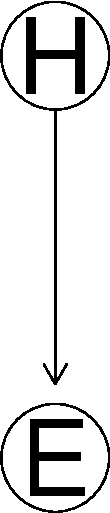
\includegraphics[width=0.6\linewidth]{conjunction-paradox2_files/figure-latex/fig:hEDAG-1} \end{center}
\caption{DAG of the simplest evidential relation}
\label{fig:hEDAG}
\end{figure}

\noindent The arrow need not have a causal interpretation. The direction
of the arrow indicates which conditional probabilities should be
supplied in the probability table. Since the arrow goes from \(H\) to
\(E\), we should specify the probabilities of the different values of
\(E\) conditional on the different values of \(H\). In addition, since
the hypothesis node has no parents, we should simply specify the prior
probabilities of the difference values of \(H\).

Back to the difficulty with conjunction. Two items of evidence, \(a\)
and \(b\), each support their own hypothesis, \(A\) and \(B\). This set
up can be represented by two directed graphs, as follows:

\mar{A: Is this what you meant?}
\ali{M: No. The two DAGS A-->a and B-->b should be one next to the other as part of the same figure. They should also look smaller and be positioned in the appropriate places.}

\begin{figure}[h]

\begin{center}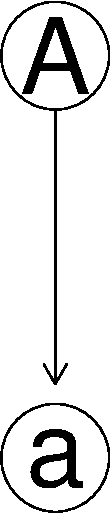
\includegraphics[width=0.6\linewidth]{conjunction-paradox2_files/figure-latex/fig:aADAG-1} \end{center}
\caption{DAG of the \textsf{a} support of the \textsf{A} hypotheses}
\label{fig:aADAG}
\end{figure}

\begin{figure}[h]

\begin{center}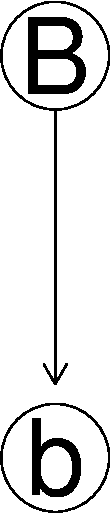
\includegraphics[width=0.6\linewidth]{conjunction-paradox2_files/figure-latex/fig:bBDAG-1} \end{center}
\caption{DAG of the \textsf{b} support of \textsf{B} the hypotheses}
\label{fig:bBDAG}
\end{figure}

\noindent The two directed graphs should be joined to represent the
conjunction \(A\wedge B\). How can this be done? Suppose for now that
claims \(A\) and \(B\) are independent. We will relax this assumption
later. The conjunction can be represented by adding a node \(AB\) in the
directed graph in Figure \ref{fig:conjunctionDAG}. The arrows go from
node \(A\) and node \(B\) into the conjunction node \(AB\). This
arrangement makes it possible to express the meaning of \(A\wedge B\)
via a probability table (Table \ref{tab:CPTconjunction}). This table
looks, essentially, like the truth table for the conjunction in
propositional logic.\footnote{The difference is that the values \(1\)
  and \(0\) stand for two different things depending on where they are
  in the table. In the columns corresponding to the nodes they represent
  node states: true and false; in the \(\textsf{Pr}\) column they
  represent the conditional probability of a given state of \(AB\) given
  the states of \(A\) and \(B\) listed in the same row. For instance,
  take a look at row two. It says: if \(A\) and \(B\) are both in states
  1, then the probability of \(AB\) being in state 0 is 0. In principle
  we could use `true' and `false' instead of 1 and 0 to represent
  states, but the numeric representation is easier to use in
  programming, which we do quite a bit in the background, so the reader
  might as well get used to this harmless ambiguity. For binary nodes,
  we will consistently use `1' and `0' for the states, it's just
  probabilities that in this case end up being extreme.}

\begin{figure}[h]

\begin{center}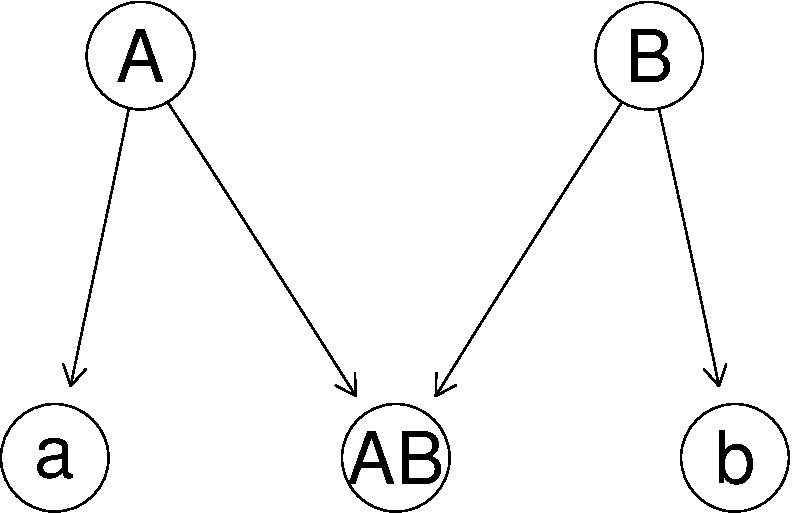
\includegraphics[width=0.6\linewidth]{conjunction-paradox2_files/figure-latex/fig:conjunctionDAG-1} \end{center}
\caption{DAG of the conjunction set-up, with the usual independence assumptions built in.}
\label{fig:conjunctionDAG}
\end{figure}

\begin{table}[h]

\begin{tabular}{lllr}
\toprule
\multicolumn{1}{c}{} & \multicolumn{1}{c}{A} & \multicolumn{1}{c}{B} & \multicolumn{1}{c}{} \\
AB &  &  & Pr\\
\midrule
1 & 1 & 1 & 1\\
0 & 1 & 1 & 0\\
1 & 0 & 1 & 0\\
0 & 0 & 1 & 1\\
1 & 1 & 0 & 0\\
0 & 1 & 0 & 1\\
1 & 0 & 0 & 0\\
0 & 0 & 0 & 1\\
\bottomrule
\end{tabular}
\caption{Conditional probability table for the conjunction node.}
\label{tab:CPTconjunction}
\end{table}

\noindent The structure of the directed graph satisfies the desired
independence assumptions. First, the two claims \(A\) and \(B\) are
probabilistically independent of one another. Their independence is
guaranteed by the fact that the conjunction node \(AB\) is a collider
and thus no information flows through it.\footnote{A more formal
  treatment of this point is provided in
  \textbf{REFER TO OTHER CHAPTER}.} Second, the supporting items of
evidence \(a\) and \(b\) are also probabilistically independent of one
another. The reason is the same: node \(AB\) blocks any flow of
information between the evidence nodes. Notably, the independence of the
items of evidence is not always explicitly stated in the formulation of
the conjunction paradox. The Bayesian network forces us to make this
explicit. This is a good thing.

With this set-up in place, the conjunction paradox arises again because
aggregation is violated. By the theory of Bayesian networks, the
directed graph in Figure \ref{tab:CPTconjunction} ensures
that:\footnote{EXPLAIN THIS POINT MORE FORMALLY} \begin{align*}
\pr{A \wedge  B \vert a \wedge b}& =\pr{A \vert a \wedge b} \times \pr{B \vert  a \wedge b \wedge A}\\
 & = \pr{A \vert a} \times \pr{B \vert  b}
 \end{align*}

\noindent  If, as is normally the case, neither \(\pr{A \vert a}\) nor
\(\pr{B \vert b}\) equal 1, then
\[\pr{A \wedge B \vert a \wedge b}< \pr{A \vert a} \;\ \& \;\ \pr{A \wedge B \vert a \wedge b} < \pr{B \vert b}. \]

\noindent Thus, even when claims \(A\) and \(B\) are sufficiently
probable given their supporting evidence \(a\) and \(b\) (for a fixed
threshold \(t\))---in symbols, \(\pr{A \vert a}>t\) and
\(\pr{B \vert b}>t\)---it does not generally follow that \(A \et B\) is
sufficiently probable given combined evidence \(a\et b\). One again, the
conjunction principle fails because aggregation fails. The difficulty
with conjunction persists.

The argument here is general and goes beyond the specific example about
aggravated assault in the previous section. The argument only assumes
that the directed graph in Figure \ref{fig:conjunctionDAG} is an
adequate representation of a situation in which two items of evidence,
\(a\) and \(b\), support their own hypothesis, \(A\) and \(B\). The
graph encodes two plausible relations of probabilistic dependence:
between hypotheses \(A\) and \(B\) and between items of evidence \(a\)
and \(b\). The theory of Bayesian network does the rest of the work.

\hypertarget{dependent-hypotheses}{%
\subsection{Dependent hypotheses}\label{dependent-hypotheses}}

What happens if the probabilistic independence between claims \(A\) and
\(B\) is dispensed with? To this end, it is enough to draw an arrow
between \(A\) and \(B\) in our directed graph. The result is displayed
in Figure \ref{fig:conjunctionDAG2}. There is an open path between the
hypotheses nodes \(A\) and \(B\) and the evidence nodes \(a\) and \(b\).
Thus, the new graph no longer guarantees the probabilistic independence
of \(A\) and \(B\), or that of \(a\) and \(b\). Items of evidence \(a\)
and \(b\) are still probabilistically independent of one another
\textit{conditional} on their respective hypothesis. That is,
\(\pr{a \vert A}=\pr{a \vert A \wedge b}\) and
\(\pr{b \vert B}=\pr{b \vert B \wedge a}\). So \(a\) and \(b\) still
counts as independent lines of evidence despite not being
(unconditionally) probabilistically independent.\footnote{Here is an
  illustration of the idea of independent lines of evidence without
  unconditional independence. Suppose the same phenomenon (say blood
  pressure) is measured by two instruments. The reading of the two
  instruments (say `high' blood pressure) should be
  \textit{probabilistically dependent} of one another. After all, if the
  instruments were both infallible and they were measuring the same
  phenomenon, they should give the exact same reading. On the other
  hand, the two instruments measuring the same phenomenon should count
  as \textit{independent lines of evidence}. This fact is rendered in
  probabilistic terms by means of probabilistic independence conditional
  on the hypothesis of interest. These ideas can be worked out more
  systematically in the language of Bayesian networks. Roughly, two
  variables are probabilistically dependent if there is an open path
  between them. On the other hand, an open path can be closed by
  conditioning on one of the variables along the path. For a more
  rigorous exposition of the notions of open and closed paths, see
  \textbf{CITE EARLIER CHAPTERS}.}

\begin{figure}[h]

\begin{center}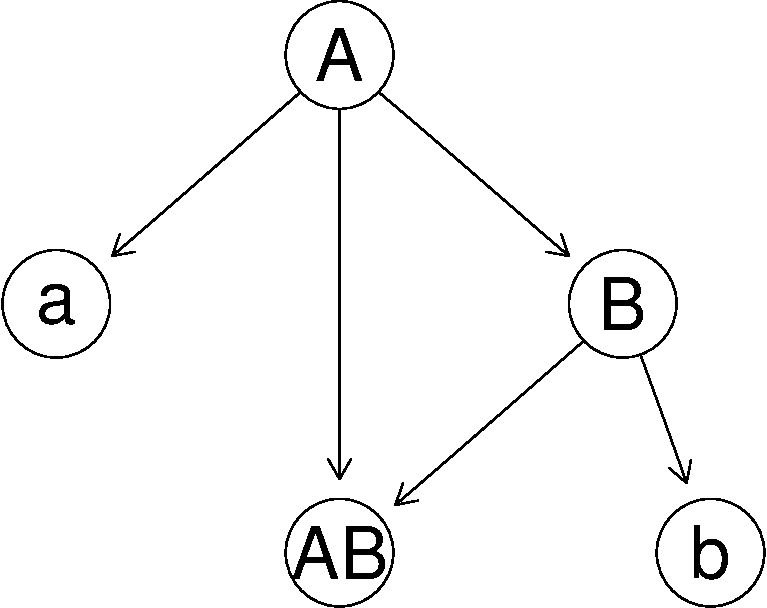
\includegraphics[width=0.6\linewidth]{conjunction-paradox2_files/figure-latex/fig:conjunctionDAG2-1} \end{center}
\caption{DAG of the conjunction set-up, without independence between $A$ and $B$.}
\label{fig:conjunctionDAG2}
\end{figure}

\ali{M: This new DAG should have the same structure as the previous one, with an extra arrow between A and B added, but all else kept the same.}

Does the difficulty with conjunction arise even without the independence
of hypotheses \(A\) and \(B\)? It does in a number of circumstances.
Suppose evidence \(a\et b\) establishes claim \(A\) and also claim
\(B\), separately, right above the probability threshold \(t\). The
graph in Figure \ref{fig:conjunctionDAG2} ensures
that:\mar{R: looks fin, although moving from P(a \& b|A\& B) to the numerator in the second line requires a bit of comment in a gloss after the derivation.}
\begin{align*}
\pr{A \wedge  B \vert a \wedge b}& =\frac{\pr{a \wedge b\vert A \wedge B}}{\pr{a\wedge b}} \pr{A \wedge B}\\
 & = \frac{\pr{a \vert A} \pr{b \vert B}}{\pr{a} \pr{b\vert a}} \times \pr{A} \pr{B \vert A}\\
   & = \frac{\pr{a \vert A}}{\pr{a}}\pr{A} \times \frac{\pr{b \vert B}}{\pr{b\vert a}} \pr{B \vert A}\\
  & = \pr{A \vert a} \times  \frac{\pr{b \vert B}}{\pr{b\vert a}} \pr{B \vert A}
 \end{align*}

\raf{M: Can you check the derivation here?}

\noindent Note that, in number of cases,
\(\nicefrac{\pr{b \vert B}}{\pr{b\vert a}} \pr{B \vert A}\) will be less
than one, or equivalently: \begin{align*}
\frac{\pr{b \vert B}}{\pr{b \vert a}}   &<  \frac{1}{\pr{B\vert A}}
\end{align*} \noindent The expression
\(\frac{\pr{b \vert B}}{\pr{b \vert a}}\) will typically be greater than
one because evidence \(b\) should provide positive support for \(B\)
even in combination with \(a\).\footnote{Because of the relations of
  independence in Figure \ref{fig:conjunctionDAG2},
  \(\nicefrac{\pr{b \vert B}}{\pr{b\vert a}}=\nicefrac{\pr{b \vert B \wedge a}}{\pr{b\vert a}}\).
  We are assuming that \(\pr{B \vert a wedge a}>\pr{B \vert a}>1\),
  which is equivalent to
  \(\nicefrac{\pr{b \vert B \wedge a}}{\pr{b\vert a}}>1\), ir in other
  words, \(b\) provides positive supports for \(B\) even in light of
  \(a\). Hence, also \(\nicefrac{\pr{b \vert B}}{\pr{b\vert a}}>1\).}
The inequality can come out true for a range of probabilities. For
instance, if \(\pr{b\vert B}=.9\),
\(\pr{b\vert a} = \pr{B \vert A} = .55\), the left-hand side is
\(\approx 1.63\) and the right-hand side is \(\approx 1.81\). If
\(\nicefrac{\pr{b \vert B}}{\pr{b\vert a}} \pr{B \vert A}<1\), then
\(\pr{A \wedge B \vert a \wedge b}< \pr{A \vert a}\).\footnote{By
  symmetric reasoning, the analogous conclusion that
  \(\pr{A \wedge B \vert a \wedge b}< \pr{B \vert b}\) follows.} There
are plenty of such cases. The general pattern is that the higher the
right side (for values above one), the lower the probability of
\(\pr{A \vert A}\) for the inequality to hold. So aggregation does not
hold generally even assuming that \(A\) and \(B\) are probabilistically
dependent. \mar{R: we still need the simulation here}

\mar{R: check calculations in chunk}
\vspace{1mm}
\footnotesize

\normalsize

\hypertarget{indepedencies-more-generally}{%
\subsection{Indepedencies more
generally}\label{indepedencies-more-generally}}

\raf{M: Move to appendix?}

The directed graphs in Figure \ref{fig:conjunctionDAG} and
\ref{fig:conjunctionDAG2} provide a compact representation of two
plausible scenarios one might have in mind in formulating the
conjunction paradox. In one scenario (Figure \ref{fig:conjunctionDAG}),
hypotheses \(A\) and \(B\), as well as items of evidence \(a\) and
\(b\), are unconditionally independent. In another scenario (Figure
\ref{fig:conjunctionDAG2}), \(A\) and \(B\) need not be independent any
longer, and \(a\) and \(b\) are only conditionally independent.

The two directed graphs encode several relationships of probabilistic
independence which it would be difficult to derive without the theory of
Bayesian networks. We list these relationships of independence below as
we will appeal to them in the rest of the chapter. The fist graph
encodes all the relationship below and the second graph encodes only a
subset of them (those marked by {[}*{]}). The symbols \(\indep\) stands
for independence.

\ali{confirm all are d-sep in the first BN, check which are d-sep in the second one and whether the d-separated in the second DAG are in fact those marked by [*].}

\raf{M: D-separtation is between variables (not values of variables). Do we need to list negations?}

\mar{R: in conditions, yeh; my getting a good grade and me working hard in class are dependent if the teacher doesn't assign grades randomly, but are independent if they do.}

\begin{align} A\indep B  \label{eq:indAB}\\
A \indep b \vert a   \label{eq:I1}\\
B \indep a \et A \vert b \label{eq:I2}\\
a\indep b \vert A\et B \label{eq:I3}  \\  
a\indep b \vert A \label{eq:I3a} [*]  \\ 
a\indep B \vert A \label{eq:I4} [*]   \\
a\indep B \vert \n A \label{eq:I4a} [*]   \\
a\indep \n B \vert A \label{eq:I4b} [*]  \\
a\indep \n B \vert \n A \label{eq:I4c} [*]  \\
b\indep A \et a \vert B \label{eq:I5} [*] \\
b\indep \n A \et a \vert B \label{eq:I5a} [*]  \\
b\indep A \et a \vert \n B \label{eq:I5b} [*] \\
b\indep \n A \et a \vert \n B \label{eq:I5c} [*]  \\
b \indep a \vert B \label{eq:I6} [*]\\
b \indep a 
\end{align}

\raf{Double check if we in fact use I3.}

\raf{M: Added the independence of a and b unconditionally. Check!}

\raf{M: We need to agree on the notation here can be confusing. We need to distinguish between variables and values of variables. Any thoughts on how to make teh notation uniform?}

\hypertarget{evidential-strength}{%
\section{Evidential Strength}\label{evidential-strength}}

The failure of the conjunction principles encountered so far are
failures of aggregation. When the probability of \(A\) and the
probability of \(B\) are both above a given threshold, the probability
of the conjunction \(A\wedge B\) usually is not. This can happen whether
or not \(A\) and \(B\) are probabilistically independent. It can also
happen whether or not the probability of \(A\) and \(B\) are conditional
on the supporting evidence. These failures of aggregation occur assuming
the standard of proof is understood as a posterior probability
threshold. Thus, aggregation cannot be justified by equating the
standard of proof to such threshold.

As an alternative, legal probabilists can think of proof standards as
decision criteria of evidential strength, specifically, how strong
strong the evidence should be in order to justify a finding of
liability. Instead of a posterior probability threshold, the standard of
proof can be modeled using a probabilistic measure of evidential
strength. Does this alternative way of modeling proof standards succeed
in solving the conjunction paradox work? To some extent, it does, but
not completely. To understand why is the task of this section.

\hypertarget{a-dilemma}{%
\subsection{A dilemma}\label{a-dilemma}}

Two common probabilistic measures of evidential strength are the Bayes
factor and the likelihood ratio. We discussed them in earlier chapters
(\textbf{REFER TO EARLIER CHAPTERS}). As will become clear later, under
plausible assumptions, these measures of evidential strength validate
one direction of the conjunction principle: aggregation. If \(a\) is
sufficiently strong evidence in favor of \(A\) and \(b\) is sufficiently
strong evidence in favor of \(B\), then \(a\wedge b\) is sufficiently
strong evidence in favor of the conjunction \(A \wedge B\). In fact, the
evidential support for the conjunction will often exceed that for the
individual claims, a point already made by Dawid (1987):

\begin{quote} suitably measured, the support supplied by the conjunction of several independent testimonies exceeds that supplied by any of its constituents.
 \end{quote}

\noindent That is, probability theory justifies this claim: if distinct
items of evidence \(a\) and \(b\) constitute sufficiently strong
evidence for claims \(A\) and \(B\), so does the conjunction
\(a\wedge b\) for the composite claim \(A\wedge B\) (although, there are
some caveats and extra assumptions for this to hold; more on this
later).

Dawid thought that vindicating aggregation was enough for the conjuction
paradox to `evaporate.' Unfortunately, we will show that on the
evidential strength interpretation of the standard of proof, the other
direction of the conjunction principle, distribution, does not hold. If
\(a \wedge b\) is sufficiently strong evidence in favor of
\(A \wedge B\), it does not follow that \(a\) is sufficiently strong
evidence in favor of \(A\) or \(b\) sufficiently strong evidence in
favor of \(B\). It is not even true that, if \(a \wedge b\) is
sufficiently strong evidence in favor of \(A \wedge B\), then
\(a\wedge b\) is sufficiently strong evidence in favor of \(A\) or
\(B\). This is odd. It would mean that, given a body of evidence, one
can establish beyond a reasonable doubt that \(A \wedge B\) (say the
defendant killed the victim \textit{and} acted intentionally) while
failing to establish one of the conjuncts.

We face a dilemma. If the standard of proof is understood as a posterior
probability threshold, the conjunction principle fails because
aggregation fails while distribution succeeds. If, on the other hand,
the standard of proof is understood as a threshold relative to
evidential strength, the conjunction principle fails because
distribution fails while aggregation succeeds. From a probabilistic
perspective, it seems impossible to capture both directions of the
conjunction principle.

In what follows, we develop more precisely the argument that, on the
evidential strength approach, (a) aggregation succeeds but (b)
distribution fails. The argument for these two claims is tedious. The
reader should arm themselves with patience or take our word for it and
jump ahead to the next section.

\hypertarget{combined-support-by-the-bayes-factor}{%
\subsection{Combined support by the Bayes
factor}\label{combined-support-by-the-bayes-factor}}

The first step in the argument shows that the combined support supplied
by multiple pieces of evidence typically exceeds the individual support
supplied by individual pieces of evidence. This claim holds for both the
Bayes factor and the likelihood ratio. We start with the Bayes factor
\(\pr{E \vert H}/\pr{E}\) as our measure of the support of \(E\) in
favor of \(H\). Since by Bayes' theorem

\[\pr{H \vert E} = \frac{\pr{E \vert H}}{\pr{E}}\times \pr{H},\]

\noindent the Bayes factor measures the extent to which a piece of
evidence increases the probability of a hypothesis. The greater the
Bayes factor (for values above one), the stronger the support of \(E\)
in favor of \(H\). Putting aside reservations about this measure of
evidential support (discussed earlier in
\textbf{REFER TO EARLIER CHAPTER}), the Bayes factor
\(\pr{E \vert H}/\pr{E}\), unlike the conditional probability
\(\pr{H \vert E}\), offers a potential way to overcome the difficulty
with conjunction by vindicating aggregation.

\hypertarget{independent-hypotheses-1}{%
\subsubsection{Independent hypotheses}\label{independent-hypotheses-1}}

Suppose items of evidence \(a\) and \(b\) positively support \(A\) and
\(B\), separately. In other words, both Bayes factors
\(\nicefrac{\pr{a \vert A}}{\pr{a}}\) (abbreviated \(BF_A\)) and
\(\nicefrac{\pr{b \vert B}}{\pr{b}}\) (abbreviated \(BF_B\)) are greater
than one. Does the combined evidence \(a \wedge b\) provide at least as
much support in favor of the joint claim \(A \wedge B\) as the
individual support by \(a\) and \(b\) in favor of \(A\) and \(B\)
considered separately? The combined support here is:
\ali{M: Check reference to independence assumptions} \begin{align*}
\frac{\pr{a \wedge b \vert A \wedge B}}{\pr{a \wedge b}} &= \frac{\pr{a \vert A}}{\pr{a}} \times \frac{\pr{b \vert B}}{\pr{b}}\\
BF_{AB} &= BF_{A} \times BF_{B}
\end{align*}

\noindent (see the appendix for a proof). This claim holds assuming
(roughly) that hypotheses \(A\) and \(B\) are independent and that items
of evidence \(a\) and \(b\) are independent. As noted earlier, these
assumptions are plausible insofar as the Bayesian network in Figure
\ref{fig:conjunctionDAG} is a plausible representation of the situation
at hand. Thus, the combined support \(BF_{AB}\) will always be higher
than the individual support so long as \(BF_{A}\) and \(BF_{B}\) are
greater than one, that is, if the individual piece of evidence
positively support their respective hypotheses.

This result generalizes beyond two pieces of evidence. Figure
\ref{fig:bfconjunction5} compares the Bayes factor of one item of
evidence, say \(\nicefrac{\pr{a \vert A}}{\pr{a}}\) with the combined
Bayes factor for five items of evidence, say
\(\nicefrac{\pr{a_1 \wedge \dots \wedge a_5 \vert A_1 \wedge \dots \wedge A_5}}{\pr{a_1\wedge \dots \wedge a_5}}\),
for different values of sensitivity and specificity of the
evidence.\footnote{The sensitivity of a piece of evidence \(e\) relative
  to a hypothesis \(H\) is \(\pr{e \vert H}\), while its specificity is
  \(\pr{\neg e | \neg H}\).} The combined Bayes factor always exceeds
the individual Bayes factors provided, as usual, the individual pieces
of evidence positively support the individual hypotheses.\footnote{The
  order is reversed if the items of evidence oppose the individual
  hypotheses. Neutral evidence results in a combined Bayes factor of 1,
  no matter the prior or the number of items of evidence} In these
circumstances, Dawid's claim that `the support supplied by the
conjunction of several independent testimonies exceeds that supplied by
any of its constituents' is vindicated.

\begin{figure}[h]

\begin{center}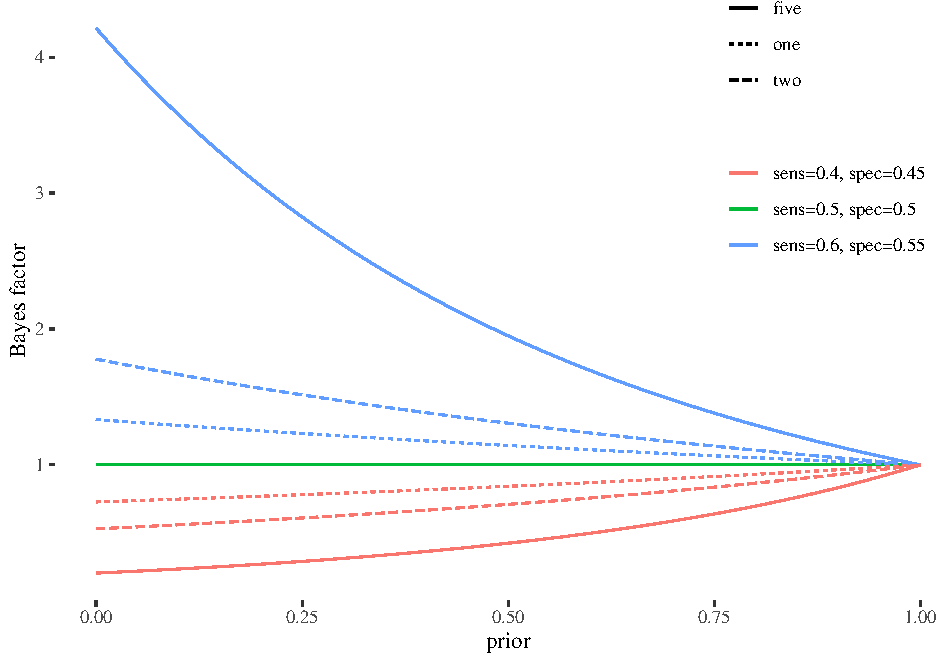
\includegraphics[width=0.9\linewidth]{conjunction-paradox2_files/figure-latex/bfconjunction5-1} \end{center}
\caption{Bayes factor for one, two and five items of evidence and the corresponding claims, given different degrees of specificity and sensitivity of the evidence. The independence assumptions in Figure \ref{fig:conjunctionDAG} hold.}
\label{fig:bfconjunction5}
\end{figure}

\hypertarget{dependent-hypotheses-1}{%
\subsubsection{Dependent hypotheses}\label{dependent-hypotheses-1}}

If \(A\) and \(B\) are not necessarily probabilistically independent as
in the Bayesian network in Figure \ref{fig:conjunctionDAG2}, the
combined Bayes factor \(BF_{AB}\) is still greater than both the
individual Bayes factor \(BF_{A}\) and \(BF_{B}\) in a number of
circumstances. To see why, first note that the following
holds:\footnote{Here is the derivation: \begin{align*}
  \frac{\pr{a \wedge b\vert A\wedge B}}{\pr{a \wedge b}} & =  \frac{\frac{ \pr{A \et B \et a \wedge b }}{\pr{A \et B}}}{\pr{a \et b}} \\ 
  & =  \frac{\frac{ \pr{A} \times \pr{B|A} \times \pr{a \vert A \wedge B} \times \pr{b \vert A \wedge B \wedge a} }{\pr{A} \times \pr{B \vert A}}}{\pr{a} \times \pr{b \vert a}} \\ 
  & =  \frac{\pr{a \vert A \wedge B} \times \pr{b \vert A \wedge B \wedge a}}{\pr{a} \times \pr{b \vert a}} \\ 
  & =^*  \frac{\pr{a |A}}{\pr{a}} \times \frac{\pr{b |B}}{\pr{b|a}} \\
  BF^{'}_{AB}& =  BF_{A}\times BF^{'}_{B} 
   \end{align*}} \begin{align*}
\frac{\pr{a \wedge b\vert A\wedge B}}{\pr{a \wedge b}} & = \frac{\pr{a |A}}{\pr{a}} \times \frac{\pr{b |B}}{\pr{b|a}} \\
BF^{'}_{AB}& =  BF_{A}\times BF^{'}_{B} 
 \end{align*}

\noindent The difference from the case of independent hypotheses is that
\(BF_B=\frac{\pr{b |B}}{\pr{b}}\) was replaced by
\(BF^{'}_B=\frac{\pr{b |B}}{\pr{b|a}}\). Since \(b\) need not be
probabilistically independent of \(a\), there is no guarantee that
\(\pr{b \vert a}=\pr{b}\). However, \(BF_B^{'}\) is usually greater than
one so long as \(b\) raises the probability of \(B\) even in conjunction
with \(a\). This is a plausible assumption to make, or else \(b\) (in
conjunction with \(a\)) would be useless evidence.\footnote{Note that
  \(BF^{'}_{B}\) is usually lower than \(BF_{B}\) because
  \(\pr{b \vert a} > \pr{b}\) (assuming, at least, \(a\) and \(b\) are
  convergent pieces of evidence;
  \textbf{REFER TO EARLIER CHAPTER ON CROSS-EXAMINATION AND CORROBORATION}.
  At the same time, \(BF^{'}_{B}\) should still be greater than one if
  \(b\) positively supports \(B\) even conditional on \(a\). Note that
  \(\frac{\pr{b \vert B}}{\pr{b\vert a}}=\frac{\pr{b \vert B \wedge a}}{\pr{b\vert a}}\),
  by independence \eqref{eq:I6}. Further, by Bayes' theorem,
  \(\pr{B \vert b \wedge a} = \frac{\pr{b \vert B \wedge a}}{\pr{b\vert a}} \times \pr{B\vert a}\),
  so \(\pr{B\vert b\et a}\) is obtained by multiplying \(\pr{B\vert a}\)
  by \(s^{'}_{B}\). In other words, the claim that
  \(\frac{\pr{b \vert B}}{\pr{b\vert a}}>1\) is equivalent to the claim
  that \(\pr{B \vert b \wedge a}> \pr{B\vert a}\). The latter is
  plausible in this context, since \(b\) should still raise the
  probability of \(B\) even in conjunction with \(a\), or else \(b\)
  would be useless evidence.} Since
\(BF^{'}_{AB} = BF_{A}\times BF^{'}_{B}\) and \(BF^{'}_B\) is greater
than one, \(BF^{'}_{AB}\) should be greater than \(BF_A\).

The argument is, in fact, symmetric. So we have: \begin{align*}
\frac{\pr{a \wedge b\vert A\wedge B}}{\pr{a \wedge b}} & =  \frac{\pr{a \vert A}}{\pr{a}} \times \underbrace{\frac{\pr{b \vert B}}{\pr{b\vert a}}}_{>1}  = \frac{\pr{b \vert B}}{\pr{b}} \times \underbrace{\frac{\pr{a \vert A}}{\pr{a\vert b}}}_{>1}
\end{align*}

\noindent As before, since \(BF^{'}_{AB} = BF_{B}\times BF^{'}_{A}\) and
\(BF^{'}_A\) is greater than one, \(BF^{'}_{AB}\) should be greater than
\(BF_B\). So, putting everything together, \(BF^{'}_{AB}\) will usually
be greater than both \(BF_A\) and \(BF_B\) even when hypotheses \(A\)
and \(B\) are dependent.

\hypertarget{section}{%
\subsection{\texorpdfstring{\textit{MOVE TO APPENDIX}}{}}\label{section}}

\ali{double check, are these d-sep in the second network?}

\raf{M: One assumption does not hold. Conditionally on A-and-B, the evidence is not independent in the DAG in Figure 2 since A-and-B is a collider node. The derivation is more complicated. See footnote.}

\begin{fact}
Assuming \eqref{eq:I3}, \eqref{eq:I4} and \eqref{eq:I6}, if $\pr{B\vert b\et a } > \pr{B\vert a}$ and $\pr{A\vert a \et b} > \pr{A \vert b}$, we have:
\[BF_{AB}> \frac{\pr{a \vert A}}{\pr{a}}, \frac{\pr{b\vert B}}{\pr{b}}\]
\end{fact}
\raf{M: What does comma mean? Fact 1 is too much formalism.}

\noindent \textbf{Argument.} First, notice the following holds given
\eqref{eq:I3} and \eqref{eq:I4}: \begin{align}
\frac{\pr{a \wedge b\vert A\wedge B}}{\pr{a \wedge b}} & =  \frac{\pr{a \vert A}}{\pr{a}} \times \frac{\pr{b \vert B}}{\pr{b\vert a}} \\
BF^{'}_{AB}& =  s_{A}\times BF^{'}_{B},  \label{eq:BFdep}
 \end{align}

\noindent  where factor \(BF_{B}= \nicefrac{\pr{b \vert B}}{\pr{b}}\)
was replaced by
\(BF^{'}_{B}=\nicefrac{\pr{b \vert B}}{\pr{b\vert a}}\).\footnote{The
  difference between \(BF_{B}\) and \(BF^{'}_{B}\) is that \(b\) need
  not be probabilistically independent of \(a\), and thus there is no
  guarantee that \(\pr{b \vert a}=\pr{b}\). In fact, \(BF^{'}_{B}\) is
  usually lower than \(BF_{B}\) because \(\pr{b \vert a} > \pr{b}\)
  (assuming, at least, \(a\) and \(b\) are convergent pieces of
  evidence; SEE DISCUSSION IN EARLIER CHAPTERS ON CROSS-EXAMINATION AND
  CORROBORATION). At the same time, \(BF^{'}_{B}\) should still be
  greater than one if \(b\) positively supports \(B\) even conditional
  on \(a\). Note that
  \(\frac{\pr{b \vert B}}{\pr{b\vert a}}=\frac{\pr{b \vert B \wedge a}}{\pr{b\vert a}}\),
  by independence \eqref{eq:I6}. Further, by Bayes' theorem,
  \(\pr{B \vert b \wedge a} = \frac{\pr{b \vert B \wedge a}}{\pr{b\vert a}} \times \pr{B\vert a}\),
  so \(\pr{B\vert b\et a}\) is obtained by multiplying \(\pr{B\vert a}\)
  by \(BF^{'}_{B}\). In other words, the claim that
  \(\frac{\pr{b \vert B}}{\pr{b\vert a}}>1\) is equivalent to the claim
  that \(\pr{B \vert b \wedge a}> \pr{B\vert a}\). The latter is
  plausible in this context, since \(b\) should still raise the
  probability of \(B\) even in conjunction with \(a\), or else \(b\)
  would be useless evidence.}
\ali{check if d-sep in this fn holds in the second bn} Hence,
\(BF^{'}_{AB}\) should be greater than either \(BF_A\) if \(BF^{'}_B\)
is\\
greater than one. Note that the reasoning behind \eqref{eq:BFdep} is
symmetric and so the assumed inequalities give the result marked by the
braces: \begin{align*}
\frac{\pr{a \wedge b\vert A\wedge B}}{\pr{a \wedge b}} & =  \frac{\pr{a \vert A}}{\pr{a}} \times \underbrace{\frac{\pr{b \vert B}}{\pr{b\vert a}}}_{>1}  = \frac{\pr{b \vert B}}{\pr{b}} \times \underbrace{\frac{\pr{a \vert A}}{\pr{a\vert b}}}_{>1}
\end{align*} So, symmetrically, we have
\(BF^{'}_{AB} = BF_{B}\times BF^{'}_{A}\), and so \(BF^{'}_{AB}\) should
be greater than either \(BF_B\) if \(BF^{'}_A\) is greater than one.

\textbf{Argument ends.}

\begin{center}\rule{0.5\linewidth}{0.5pt}\end{center}

\raf{M: Need to introduce simulations, illustrate results for aggregation and BF without independence here}

\hypertarget{combined-support-by-the-likelihood-ratio}{%
\subsection{Combined support by the likelihood
ratio}\label{combined-support-by-the-likelihood-ratio}}

The Bayes factor can be replaced by the likelihood ratio, another
probabilistic measure of evidential support, extensively discussed in
\textbf{REFER TO Chapter XXX \todo{REF}}. The likelihood ratio compares
the probability of the evidence on the assumption that a hypothesis of
interest is true and the probability of the evidence on the assumption
that the negation of the hypothesis is true, that is,
\(\nicefrac{\pr{E \vert H}}{\pr{E \vert \neg H}}\). We can think of the
the likelihood ratio as the following:

\[\frac{\textit{sensitivity}}{\textit{1- specificity}}\]

\noindent The greater the likelihood ratio (for values above one), the
stronger the evidential support in favor of the hypothesis (as
contrasted to the its negation). Unlike the Bayes factor, the likelihood
ratio is not sensitive to the prior probability of the hypothesis of
interest so long as sensitivity and specificity are not sensitive to the
prior.\footnote{This point is debated in the literature \textbf{CITE}.
  Further, we will see that specificity is sensitive to prior
  probabilities in the case of combined hypotheses.}

Does the combined support measured by the combined likelihood ratio
\(\nicefrac{\pr{a\wedge b \vert a\wedge B}}{\pr{a \wedge b \vert \neg (A\wedge B)}}\)
exceed the individual support measured by the individual likelihood
ratios \(\nicefrac{\pr{a \vert A}}{\pr{a \vert \neg A}}\) and
\(\nicefrac{\pr{b \vert B}}{\pr{b \vert \neg B}}\)? Under suitable
assumptions, the answer is positive. So, details aside, Bayes factor and
likelihood ratio agree on this point. The argument for the likelihood
ratio, however, is more laborious.

\hypertarget{combined-sensitivity-and-specificity}{%
\subsubsection{Combined sensitivity and
specificity}\label{combined-sensitivity-and-specificity}}

First, we compute the numerator and denominator of the combined
likelihood ratio. The numerator is easy. It results from multiplying the
sensitivity of the individual items of evidence, \(a\) and \(b\),
relative to their respective hypotheses, \(A\) and \(B\):\footnote{\begin{align*}
  \pr{a \wedge b\vert A\wedge B} & =  \frac{\pr{A \et B \et a\et b}}{\pr{A \et B}}
  &\mbox{\,\,\,\,\,\,\,\,\,\,\,\,\, (conditional probability)}
  \\
  &= \frac{   \pr{A} \times \pr{B\vert A} \times \pr{a \vert A \wedge B} \times \pr{b \vert A \wedge B \wedge a} }{\pr{A} \times \pr{B \vert A}}
  &\mbox{\,\,\,\,\,\,\,\,\,\,\,\,\, (chain rule)}
  \\
  & = \frac{\pr{A} \times \pr{B \vert A} \times \pr{a \vert A} \times \pr{b \vert B}}{\pr{A}  \times \pr{B \vert A}} 
  &\mbox{\,\,\,\,\,\,\,\,\,\,\,\,\, (independencies \eqref{eq:I3a} and \eqref{eq:I5})}
  \\
  & = \pr{a \vert A} \times \pr{b \vert B} 
  &\mbox{\,\,\,\,\,\,\,\,\,\,\,\,\, (algebraic manipulation)}
   \end{align*}} \begin{align*}
\pr{a \wedge b\vert A\wedge B} & =  \pr{a \vert A} \times \pr{b \vert B} 
 \end{align*} \noindent Call this \textit{combined sensitivity}. The
denominator of the combined likelihood ratio is more complicated, mostly
because of the presence of \(\neg (A \wedge B)\) as a
condition:\footnote{\begin{align*}
  \pr{a \et b\vert \neg (A\et B)} & = \frac{\pr{a \et b \et \neg (A\et B)}}{\pr{\neg (A \et B)}} 
  &\mbox{\,\,\,\,\,\,\,\,\,\,\,\,\, (conditional probability)}\\
  & = \frac{\pr{a \et b \et \neg A\et B} +  \pr{a \et b \et A\et \neg B} + \pr{a \et b \et \neg A\et \neg B}  }{\pr{\neg A \et B} + \pr{A \et \neg B} + \pr{\neg A \et \neg B} } 
  &\mbox{\,\,\,\,\,\,\,\,\,\,\,\,\, (logic \& additivity)}
  \end{align*} \noindent Now consider the first summand from the
  numerator: \begin{align*}
  \pr{a \et b \et \neg A\et B} & = \pr{\n A} \pr{B \vert \n A} \pr{a \vert \n A \et B} \pr{b\vert a \et \n A \et B} &\mbox{\,\,\,\,\,\,\,\,\,\,\,\,\, (chain rule)} \\ & = 
  \pr{\neg A}\pr{B \vert \neg A} \pr{a \vert \neg A}\pr{b \vert B}
  &\mbox{\,\,\,\,\,\,\,\,\,\,\,\,\, (independencies \eqref{eq:I4a} and \eqref{eq:I5a})} \\
  \end{align*} The simplification of the other two summanda is analogous
  (albeit with slightly different independence
  assumptions---\eqref{eq:I4b} and \eqref{eq:I5b} for the second one and
  \eqref{eq:I4c} and \eqref{eq:I5c} for the third. Once we plug these
  into the denominator formula we get: \begin{align*}
  \pr{a \et b\vert \neg (A\et B)} & = \frac{\pr{\neg A}\pr{B \vert \neg A} \pr{a \vert \neg A}\pr{b \vert B} + \pr{A}\pr{\neg B \vert A} \pr{a \vert A }\pr{b \vert \neg B} + \pr{\neg A}\pr{\neg B \vert \neg A } \pr{a \vert \neg A}\pr{b \vert \neg B}}{\pr{\neg A}\pr{B \vert \neg A} + \pr{A}\pr{\neg B \vert A } + \pr{\neg A}\pr{\neg B \vert \neg A} }  
   \end{align*}}

\scalebox{.85}{\parbox{1\linewidth}{
\begin{align*}
\pr{a \et b\vert \neg (A\et B)} & = \frac{\pr{\neg A}\pr{B \vert \neg A} \pr{a \vert \neg A}\pr{b \vert B} + \pr{A}\pr{\neg B \vert A} \pr{a \vert A }\pr{b \vert \neg B} + \pr{\neg A}\pr{\neg B \vert \neg A } \pr{a \vert \neg A}\pr{b \vert \neg B}}{\pr{\neg A}\pr{B \vert \neg A} + \pr{A}\pr{\neg B \vert A } + \pr{\neg A}\pr{\neg B \vert \neg A} }  
 \end{align*}
}}

Call this \textit{combined specificity}. The two equalities holds
whether or not \(A\) and \(B\) are probabilistically independent. So
both directed graphs in Figure \ref{fig:conjunctionDAG} and Figure
\ref{fig:conjunctionDAG2} validate these claims.

\hypertarget{equal-probability-and-independence}{%
\subsubsection{Equal probability and
independence}\label{equal-probability-and-independence}}

Many variables are at play here. Unlike with the Bayes factor, it is not
easy to compare the combined evidential support and the individual
support. For illustrative purpose, we simplify. Let the sensitivity and
specificity for the items of evidence involved be the same and equal
\(x\). Let also \(A\) and \(B\) be probabilistically independent in
agreement with the directed graph in Figure \ref{fig:conjunctionDAG}. In
this simplified set-up, the combined likelihood ratio reduces to the
following, where \(\pr{A}=k\) and \(\pr{B}=t\): \begin{align*}
\frac{\pr{a \wedge b \vert A\wedge B}}{\pr{a \et b\vert \neg (A\et B)}} & = \frac{x^2}{\frac{(1-k)t(1-x)x + k(1-t)x(1-x) + (1-k)(1-t)(1-x)(1-x)}{ \left(1-k\right) t +\left(1-t\right) k+\left(1-k\right) \left(1-t\right)}}
 \end{align*}

\noindent The combined likelihood ratio can now be easily plotted. As
Figure \ref{fig:jointLRMarcello} shows, the combined likelihood ratio
always exceeds the individual likelihood ratios whenever they are
greater than one (or in other words, as is usually assumed, the two
pieces of evidence provide positive support for their respective
hypotheses). Interestingly, we notice that the combined likelihood ratio
varies deepening on the prior probabilities \(\pr{A}\) and \(\pr{B}\).

\begin{figure}

\begin{center}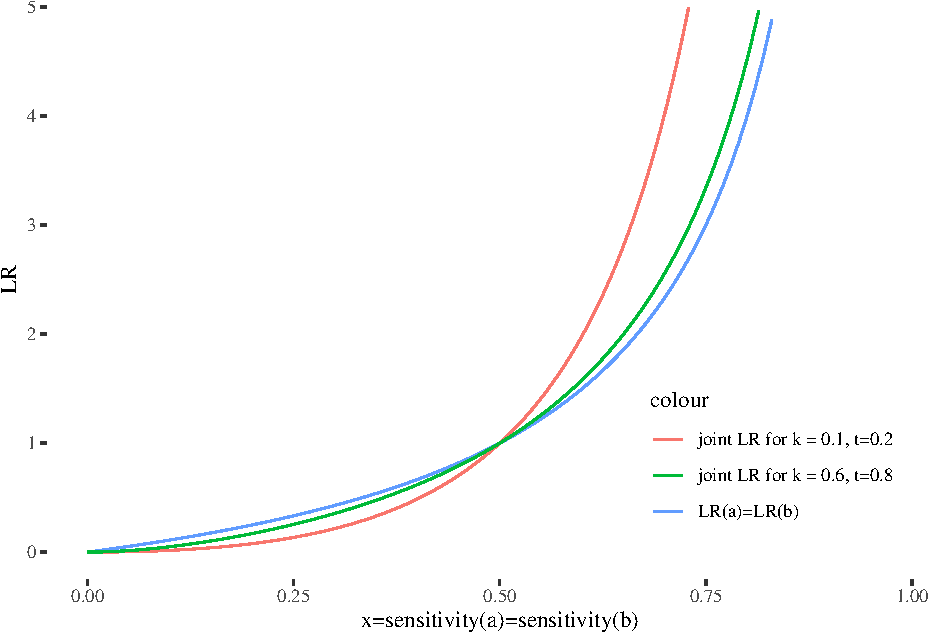
\includegraphics[width=0.9\linewidth]{conjunction-paradox2_files/figure-latex/unnamed-chunk-3-1} \end{center}

\caption{Combined likelihood ratios exceeds individual Likelihood ratios as soon as sensitivity is above .5. Changes in the prior probabilities $t$ and $k$ do not invalidate this result.}
\label{fig:jointLRMarcello}
\end{figure}

As with the Bayes factor, the combined likelihood ratio exceeds the
individual likelihood ratios. However, the graph only covers cases in
which the two pieces of evidence have the same sensitivity and
specificity and hypotheses \(A\) and \(B\) are probabilistically
independent. What happens when these two assumptions are relaxed?

\hypertarget{more-complex-scenarios-needs-simulation}{%
\subsubsection{More complex scenarios -- NEEDS
SIMULATION}\label{more-complex-scenarios-needs-simulation}}

If the items of evidence have different levels of sensitivity and
specificity, the combined likelihood ratio never goes below the lower of
the two individual likelihood ratios, but can be lower than the higher
one. \raf{M: Need to add simulation results to make this argument 
fully general and drop all the simplifying assumptions (.e.g. independence or equiprobability)}
If the composite likelihood ratio behaves differently than the Bayes
factor in that it is greater than the lower of the individual likelihood
ratios, rather than being greater than both of them, Dawid's claim that
`the support supplied by the conjunction of several independent
testimonies exceeds that supplied by any of its constituents' still
holds.

\hypertarget{section-1}{%
\subsection{\texorpdfstring{\textit{MOVE TO APPENDIX}}{}}\label{section-1}}

\begin{fact} If independence assumptions \ali{check whic of these d-sep hold in the first and in the second BN}  \eqref{eq:I3a}, \eqref{eq:I4a},  \eqref{eq:I4b}, \eqref{eq:I4c}, \eqref{eq:I5}, \eqref{eq:I5a}, \eqref{eq:I5b}   and \eqref{eq:I5c} hold, the combined likelihood ratio is:
 \begin{align}\label{eq:jointLR}
\frac{\pr{a \wedge b \vert A\wedge B}}{\pr{a \et b\vert \neg (A\et B)}} & = \frac{\pr{a \vert A} \times \pr{b \vert B}}{\frac{\pr{\neg A}\pr{B \vert \neg A} \pr{a \vert \neg A}\pr{b \vert B} + \pr{A}\pr{\neg B \vert A} \pr{a \vert A }\pr{b \vert \neg B} + \pr{\neg A}\pr{\neg B \vert \neg A } \pr{a \vert \neg A}\pr{b \vert \neg B}}{\pr{\neg A}\pr{B \vert \neg A} + \pr{A}\pr{\neg B \vert A } + \pr{\neg A}\pr{\neg B \vert \neg A} } }
 \end{align}
\noindent If, further the hypotheses are independent in the sense of  \label{eq:indAB} this reduces to:
 \begin{align}\label{eq:jointLR2}
\frac{\pr{a \wedge b \vert A\wedge B}}{\pr{a \et b\vert \neg (A\et B)}} & = \frac{\pr{a \vert A} \times \pr{b \vert B}}{\frac{\pr{\neg A}\pr{B} \pr{a \vert \neg A}\pr{b \vert B} + \pr{A}\pr{\neg B} \pr{a \vert A }\pr{b \vert \neg B} + \pr{\neg A}\pr{\neg B} \pr{a \vert \neg A}\pr{b \vert \neg B}}{\pr{\neg A}\pr{B} + \pr{A}\pr{\neg B} + \pr{\neg A}\pr{\neg B} } }
 \end{align}
 \end{fact}

\noindent \textbf{Argument.} The numerator can be computed as follows:
\begin{align*}
\pr{a \wedge b\vert A\wedge B} & =  \frac{\pr{A \et B \et a\et b}}{\pr{A \et B}}
&\mbox{\,\,\,\,\,\,\,\,\,\,\,\,\, (conditional probability)}
\\
&= \frac{   \pr{A} \times \pr{B\vert A} \times \pr{a \vert A \wedge B} \times \pr{b \vert A \wedge B \wedge a} }{\pr{A} \times \pr{B \vert A}}
&\mbox{\,\,\,\,\,\,\,\,\,\,\,\,\, (chain rule)}
\\
& = \frac{\pr{A} \times \pr{B \vert A} \times \pr{a \vert A} \times \pr{b \vert B}}{\pr{A}  \times \pr{B \vert A}} 
&\mbox{\,\,\,\,\,\,\,\,\,\,\,\,\, (independencies \eqref{eq:I3a} and \eqref{eq:I5})}
\\
& = \pr{a \vert A} \times \pr{b \vert B} 
&\mbox{\,\,\,\,\,\,\,\,\,\,\,\,\, (algebraic manipulation)}
 \end{align*}

The numerator clearly does not depend on the prior probability of
\(A\wedge B\). We call it \textit{combined sensitivity}, and given the
independence assumptions it simply results from multiplying the
sensitivity of the individual items of evidence, \(a\) and \(b\),
relative to their respective hypotheses, \(A\) and \(B\).

The denominator is more involved:

\scalebox{.85}{\parbox{1\linewidth}{
\begin{align*}
\pr{a \et b\vert \neg (A\et B)} & = \frac{\pr{a \et b \et \neg (A\et B)}}{\pr{\neg (A \et B)}} 
&\mbox{\,\,\,\,\,\,\,\,\,\,\,\,\, (conditional probability)}\\
& = \frac{\pr{a \et b \et \neg A\et B} +  \pr{a \et b \et A\et \neg B} + \pr{a \et b \et \neg A\et \neg B}  }{\pr{\neg A \et B} + \pr{A \et \neg B} + \pr{\neg A \et \neg B} } 
&\mbox{\,\,\,\,\,\,\,\,\,\,\,\,\, (logic \& additivity)}
\end{align*}
}}

\noindent Now consider the first summand from the numerator:
\begin{align*}
\pr{a \et b \et \neg A\et B} & = \pr{\n A} \pr{B \vert \n A} \pr{a \vert \n A \et B} \pr{b\vert a \et \n A \et B} &\mbox{\,\,\,\,\,\,\,\,\,\,\,\,\, (chain rule)} \\ & = 
\pr{\neg A}\pr{B \vert \neg A} \pr{a \vert \neg A}\pr{b \vert B}
&\mbox{\,\,\,\,\,\,\,\,\,\,\,\,\, (independencies \eqref{eq:I4a} and \eqref{eq:I5a})} \\
\end{align*}

The simplification of the other two summanda is analogous (albeit with
slightly different independence assumptions---\eqref{eq:I4b} and
\eqref{eq:I5b} for the second one and \eqref{eq:I4c} and \eqref{eq:I5c}
for the third. Once we plug these into the denominator formula we get:

\scalebox{.85}{\parbox{1\linewidth}{
\begin{align*}
\pr{a \et b\vert \neg (A\et B)} & = \frac{\pr{\neg A}\pr{B \vert \neg A} \pr{a \vert \neg A}\pr{b \vert B} + \pr{A}\pr{\neg B \vert A} \pr{a \vert A }\pr{b \vert \neg B} + \pr{\neg A}\pr{\neg B \vert \neg A } \pr{a \vert \neg A}\pr{b \vert \neg B}}{\pr{\neg A}\pr{B \vert \neg A} + \pr{A}\pr{\neg B \vert A } + \pr{\neg A}\pr{\neg B \vert \neg A} }  
 \end{align*}
}}

\noindent  \eqref{eq:jointLR2} is easily obtained from
\eqref{eq:jointLR} by \label{eq:indAB}.\\
\textbf{Argument ends.}

\hypertarget{vindicating-aggregation}{%
\subsection{Vindicating aggregation}\label{vindicating-aggregation}}

The fact that---for both the Bayes faxctor and the likelihood ratio--the
support supplied by the conjunction usually exceeds the support supplied
by individual items of evidence can be used to justify aggregation. The
argument, however, is not straightforward. Aggregation is a principle
about the standard of proof. So, in order to vindicate aggregation, the
standard of proof should be understood in terms of evidential strength.
But how this should be done is not obvious.

Here is what should be obvious. If the decision criterion is formulated
in terms of evidential strength instead of posterior probabilities,the
standard of proof should no longer be formalized as a posterior
probability threshold, but rather as a threshold for the Bayes factor or
the likelihood ratio. The threshold should no longer be a probability
between 0 and 1, but a number somewhere above one. The greater this
number, the more stringent the standard of proof, for any value above
one. In criminal trials, for example, the rule of decision would be:
guilt is proven beyond a reasonable doubt if and only if the evidential
support in favor of \(H\)---as measured by the Bayes factor
\(\nicefrac{\pr{E \vert H}}{\pr{E}}\) (or by the likelihood ratio
\(\nicefrac{\pr{E\vert H}}{\pr{E \vert \n H}}\))---meets a suitably high
threshold \(t_{BF}\) (\(t_{LR}\)). The question at this point is, how do
we identify the appropriate threshold? The answer to this question is
not obvious. \todo{will at some point take a look at "Bayesian Choice"}

\hypertarget{variable-threhsold}{%
\subsubsection{Variable threhsold}\label{variable-threhsold}}

We first articulate an approach that is a non-starter. It is useful to
understand why this appropach does not work to formulate a more
promising approach. A threshold on evidential strength can be derived
from the threshold on posterior probability. The advantage of the
posterior probability threshold is that its stringency can be determined
in a decision-theoretic manner via the minimization of expected costs.
(\textbf{REFER TO ERALIER CHAPPER}\}) Something analogous can be done
for the Bayes factor or the likelihood ratio. One option is to derive a
threshold for the Bayes factor and the likelihood ratio, call these
thresholds \(t_{BF}\) or \(t_{LR}\), from a thresholds \(t\) on the
posterior probability. This is easy to do.

Consider threshold \(t_{BF}\) first. Since
\(\mathsf{posterior }=\mathsf{ Bayes factor }\times \mathsf{ prior}\),
the Bayes factor threshold can be determined as follows:
\begin{align*}t_{BF} & = \frac{t}{\textsf{prior}}
\end{align*}

\noindent The higher the prior probability, the lower \(t_{BF}\). So
threshold \(t_{BF}\) would be dependent on the prior probability of the
hypothesis of interest. Whether this is a desirable property for a
decision threshold can be questioned, but a similar point holds about
the standard posterior threshold \(t\): the higher the prior
probability, the easier to meet this threshold.

The same strategy works for the threshold \(t_{LR}\). By the odds
version of Bayes' theorem, \begin{align*}
\textsf{posterior odds} & = \textsf{likelihood odds} \times \textsf{prior odds},
\end{align*} and thus
\begin{align*}\frac{\textsf{posterior odds}}{\textsf{prior odds}} = \textsf{likelihood ratio}.
\end{align*} If the posterior ratio is fixed at, say \(t/1-t\),
\(t_{LR}\) can be obtained as follows:
\begin{align*}t_{LR} & = \frac{\nicefrac{t}{1-t}}{\textsf{prior odds}}.
\end{align*}

\noindent Just as the Bayes factor, the likelihood ratio threshold will
vary with the prior. The higher the prior, the lower the likelihood
ratio threshold.

This approach incur two shortcoming. First, the variable threshold for
Bayes factor or the likelihood ratio is parasitic on the posterior
probability threshold. So if there are reasons to reject the posterior
probability threshold, these reasons would also apply to the other
thresholds. Second---and more to the point---aggregation still fails for
\(t_{BF}\) and \(t_{LR}\) just like it failed in case of the threshold
for posterior probabilities. There will be cases in which the conjuncts
taken separately satisfy the decision standard \(t_{BF}\) or \(t_{LR}\),
while the conjunction does not.
\raf{Question: how does Kaplow think about it? Does he only derive threshold for the ultimate claim? I don't remember now.}
The culprit here is the fact that these thresholds are prior-dependent.
So \(t_{BF}\) and \(t_{LR}\) will have different absolute values when
applied to to individual claims \(A\) and \(B\) compared to the
composite claim \(A \wedge B\), since the prior probability of a
composite claim differs from that of individual claims. The formal
details can be found in \textbf{REFER TO APPENDIX}.

Perhaps, this is not the path that the proponent of the evidential
strength approach would take anyway. If the evidential strength
threshold mirrors the posterior threshold, it should not be surprising
that it runs into similar problems. So what would happen if, instead,
the evidential strength threshold was kept fixed and did not depend on
priors?

\hypertarget{to-be-moved-to-appendix}{%
\paragraph{TO BE MOVED TO Appendix}\label{to-be-moved-to-appendix}}

Now, we would like a standard of proof to be in principle applicable to
all factual claims under consideration. In particular, if we consider a
conjunction \(A\et B\), we should have a standard that makes sense not
only when applied to \(A\et B\), but also when applied to \(A \et B\).
But now notice that in the current set-up evidential strength thresholds
vary with priors, and clearly the priors for \(A\) and \(B\) will differ
from the priors on \(A\et B\). This suggests that as long as we want
\(t_{BF}\) and \(t_{LR}\) to be decision-theoretically justified by
being derived from a decision-theoretically justified posterior
probability threshold, the thresholds for individual claims
(\(t_{BF}^A\) and \(t_{LR}^A\)) will differ from the thresholds for the
composite claim, \(t_{BF}^{A\wedge B}\) and \(t_{LR}^{A\wedge B}\) .

The conjunction principles formulated in terms of BF and LR would boil
down to:
\begin{align*} \frac{\pr{a \vert A }}{\pr{a}}>t^A_{BF} &\mbox{ and } 
\frac{\pr{ b \vert B}}{\pr{b}}>t^B_{BF} \mbox{ iff } 
\frac{\pr{a \et b \vert A \et B}}{\pr{a \et b}}>t^{A\wedge B}_{BF} \\
 \frac{\pr{a \vert A }}{\pr{a \vert \n A}}>t^A_{LR} &\mbox{ and } 
\frac{\pr{ b \vert B}}{\pr{b\vert B}}>t^B_{LR} \mbox{ iff } 
\frac{\pr{a \et b \vert A \et B}}{\pr{a \et b\vert \n (A \et B)}}>t^{A\wedge B}_{LR} \\
\end{align*}

Now, consider the individual claims \(A\) and \(B\) and their
conjunction \(A \wedge B\), assuming the independence relations required
for Facts \ali{REF} and \ali{REF} hold. Consider a posterior threshold
of \(.95\) as might be appropriate in a criminal case.

\todo{please use nicefrac for inline fractions}

If \(A\) and \(B\) both have a prior probability of, say \(.1\), the
threshold \(t^A_{BF}=t_{BF}^B=\nicefrac{.95}{.1}=9.5\) for \(A\) or
\(B\) individually. The composite claim \(A \wedge B\) will be
associated with the threshold
\(t^{A\wedge B}_{BF}=\nicefrac{.95}{(.1\times .1)}=95\), a much higher
value. But if each individual claim meets its Bayes factor threshold of
9.5 and the two claims are independent, the joint Bayes factor would
result from the multiplication of the individual Bayes factors, that is,
\(9.5 \times 9.5=90.25\). This is not quite enough to meet
\(t^{A\wedge B}_{BF}=95\).

The difference grows as (i) the prior probability of the individual
claims decreases, (ii) as the posterior threshold \(t\) decreases, and
(iii) as the number of constituents claims increases. For two
constituents, the combined Bayes factor remains only \(5\%\) below the
value needed to meet \(t_{BF}^{A\wedge B}\). The difference at here is
between \(t_{BF}^{A\wedge B}=\nicefrac{.95}{p^2}\) and
\(t_{BF}^{A}*t_{BF}^{B}=(\nicefrac{.5}{p})^{2}\). Note that
\(\frac{\nicefrac{.95}{p^2} - (\nicefrac{.5}{p})^{2}}{\nicefrac{.95}{p^2}}=.05\),
for any value of the prior \(p\). Given five constituent claims,
\(\frac{\nicefrac{.95}{p^5} - (\nicefrac{.95}{p})^{5}}{\nicefrac{.95}{p^5}}=.18\).
Now, say \(t=.5\). Even with just two claims,
\(t^{A\wedge B}_{BF}=.5/(.1*.1)=50\), but
\(t^A_{BF}*t_{BF}^B=(.5/.1)*(.5/.1)=25\), only half of the required
value.

An analogous point will hold for the likelihood ratio. Say \(A\) and
\(B\) have prior probabilities of \(.2\) and \(.3\) respectively. On
this approach, the likelihood ratio threshold for \(A\) and \(B\) will
be \(t_{LR}^{A}\approx 76\) and \(t_{LR}^{B}a\approx 44\). The
likelihood ratio threshold for the composite claim \(A \wedge B\) will
be \(t^{A\wedge B}_{LR}\approx 297\). Now suppose the individual
likelihood ratios meet their threshold and respective sensitivities and
specificities are identical. For \(t_{LR}^{A}\) to be met, evidence
\(a\) should have sensitivity of at least 0.988. For \(t_{LR}^{B}\) to
be met, evidence \(b\) should have sensitivity 0.978. Now with these
separate sensitivies, The combined likelihood ratio equals about 145,
far short that what the threshold \(t^{A\wedge B}_{LR}\) requires,
namely a likelihood ratio of 297.

Things don't get better with a lower posterior threshold. Say \(t= .5\),
as might be appropriate in a civil case. The likelihood ratio thresholds
for \(A\) and \(B\) will be \(t_{LR}^{A}\approx 4\) and
\(t_{LR}^{B}a\approx 2.3\). The likelihood ratio threshold for the
composite claim \(A \wedge B\) will be
\(t^{A\wedge B}_{LR}\approx 15.6\). To ensure that \(t_{LR}^{A}\) is
met, evidence \(a\) should have a sensitivity of at least 0.8, and to
ensure that \(t_{LR}^{B}\) is met, evidence \(b\) should have a
sensitivity of at least 0.7. To ensure that \(t_{LR}^{B}\) is met,
evidence \(b\) should have a sensitivity of at least 0.7. With these
parameters, the combined likelihood ratio equals about 5, far short that
what the threshold \(t^{A\wedge B}_{LR}\) requires, namely a likelihood
ratio of 15.

\hypertarget{fixed-threshold}{%
\subsubsection{Fixed threshold}\label{fixed-threshold}}

The alternative here is to fix the evidential strength threshold
regardless of the prior probability of the claim of interest. This
raises the difficult question of how to fix the threshold irrespective
of the priors. Standard decision theory can no longer be used. Still,
assuming this question can be satisfactorily answered, the fixed
threshold approach manages to vindicate aggregation. This is a
significant improvement.

If the standard of proof is formalized using a fixed threshold for the
Bayes factor or for the likelihood ratio, the conjunction principle
would boil down to one of these:

\begin{align*} \frac{\pr{a \vert A }}{\pr{a}}>t_{BF} &\mbox{ and } 
\frac{\pr{ b \vert B}}{\pr{b}}>t_{BF} \mbox{ iff } 
\frac{\pr{a \et b \vert A \et B}}{\pr{a \et b}}>t_{BF} \\
 \frac{\pr{a \vert A }}{\pr{a \vert \n A}}>t_{LR} &\mbox{ and } 
\frac{\pr{ b \vert B}}{\pr{b\vert B}}>t_{LR} \mbox{ iff } 
\frac{\pr{a \et b \vert A \et B}}{\pr{a \et b\vert \n (A \et B)}}>t_{LR} \\
\end{align*}

\noindent The left-to-right direction---aggregation---holds for any
thresholds \(t_{BF}\) or \(t_{LR}\) greater than one. As shown
previously, the combined evidential support is usually greater than the
individual evidential support, whether it is measured in terms of the
Bayes factor or the likelihood ratio. This is an improvement.
Aggregation could not be justified using posterior probabilities
\(\pr{A \vert a}\) and \(\pr{B \vert b}\) nor could it be justified
generally using a variable Bayes factor threshold. So it is an advantage
of the fixed evidential strength threshold approach that it can justify
this direction of the conjunction principle.

However, the right-to-left direction---distribution---has now become
problematic. Two versions of the distribution principle can be
distinguished: \begin{align}
\text{If S[$a \wedge b, A\wedge B$], then S[$a, A$] and S[$b, B$].} \tag{DIS1}\\
 \text{If S[$a \wedge b, A\wedge B$], then S[$a \wedge b, A$] and S[$a \wedge b, B$].} \tag{DIS2}
\end{align}

\noindent Let us start with (DIS1) first, still working with the
independence assumptions in the background for the sake of simplicity.
Suppose the combined Bayes factor,
\(\frac{\pr{a \et b \vert A \et B}}{\pr{a \et b}}\), barely meets the
threshold. The individual support, say
\(\frac{\pr{a \vert A}}{\pr{a}}\), could be still below the threshold
unless \(\frac{\pr{b \vert B}}{\pr{b}}=1\) (which should not happen if
\(b\) positively supports \(B\)).

The problem for likelihood ratio is analogous. For suppose evidence
\(a \et b\) supports \(A \et B\) to the required threshold \(t\). The
threshold in this case should be some order of magnitude greater than
one. If the combined likelihood ratio meets the threshold \(t_{LR}\),
one of the individual likelihood ratios may well be below \(t_{LR}\).
So---if the standard of proof is interpreted using evidential support
measured by the likelihood ratio---even though the conjuction
\(A \et B\) was proven according to the desired standard, one of
individual claims might not. (DIS1) in some cases fails.

Perhaps, the problem was with (DS1). Could this principle be rejected?
Maybe it is not as essential as we thought at first. Since the evidence
is not held constant, the support supplied by \(a\wedge b\) could be
stronger than that supplied by \(a\) and \(b\) individually. So even
when the conjunction \(A \wedge B\) is established to the requisite
standard given evidence \(a\wedge b\), it might still be that \(A\) does
not meet the requisite standard (given \(a\)) nor does \(B\) (given
\(b\)). Or at least one might try to argue so.

(DS2) is less controversial, as it holds the evidence constant. This
principle is harder to deny: one would not want to claim that, holding
fixed evidence \(a\wedge b\), establishing the conjunction might not be
enough for establishing one of the conjuncts. It seems that any
formalization of the standard of proof should obey (DIS2). Yet, (DIS2)
also fails both for Bayes factor and likelihood ratio. After all, if
\(A\) and \(B\) are probabilistically independent, (DIS1) and (DIS2) are
in fact equivalent, so the counterexamples to (DIS1) work also against
(DS2).

Curiously, on the fixed evidential strength threshold approach, no
matter whether one uses Bayes factor or likelihood ratio, there would be
cases in which, even though the conjunction \(A\et B\) is established by
the desired standard of proof, one of the individual claims fails to
meet the standard. This is odd, to say the least.

\mar{R:I don't think this argument worked, we can discuss this. Commented out}
\raf{M: What exactly did not work in the argument that you commented out? It 
is just a restatement of the earlier point.}

\raf{M: This section seems to be missing a lot of the reasoning 
that was commented out. Is this still comprehensible? 
Not sure I can follow. Seems too brief.}

\hypertarget{the-comparative-strategy}{%
\section{The comparative strategy}\label{the-comparative-strategy}}

Instead of thinking in terms of absolute thresholds---whether relative
to posterior probabilities, the Bayes factor or the likelihood
ratio---the standard of proof can be understood comparatively. This
suggestion has been advanced by Cheng (2012) following the theory of
relative plausibility by
\textbf{REFERENCE TO ALLEN AND PARDO HERE}.\todo{Which one?} Say the
prosecutor or the plaintiff puts foward a hypothesis \(H_p\) about what
happened. The defense offers an alternative hypothesis, call it \(H_d\).
On this approach, rather than directly evaluating the support of \(H_p\)
given the evidence and comparing it to a threshold, we compare the
support that the evidence provides for two competing hypotheses \(H_p\)
and \(H_d\), and decide for the one for which the evidence provides
better support.

It is controversial whether this is what happens in all trial
proceedings, especially in criminal trials, if one thinks of \(H_d\) as
a substantial account of what has happened. The defense may elect to
challenge the hypothesis put foward by the other party without proposing
one of its own. For example, in the O.J.~Simpson trial the defense did
not advance its own story about what happened, but simply argued that
the evidence provided by the prosecution, while significant on its face
to establish OJ's guilt, was riddled with problems and deficencies. This
defense strategy was enough to secure an acquittal. So, in order to
create a reasonable doubt about guilt, the defense does not always
provide a full-fledged alternative hypothesis. The supporters of the
comparative approach, however, will respond that this could happen in a
small number of cases, even though in general---especially for tactical
reasons---the defense will provide an alternative hypothesis. And even
such cases can be construed as involving a defense hypothesis, one that
is simply equivalent to the negation of \(H_p\).

Setting aside this controversy for the time being, let's first work out
the comparative strategy using posterior probabilities. More
specifically, given a body of evidence \(E\) and two competing
hypotheses \(H_p\) and \(H_d\), the probability \(\pr{H_p \vert E}\)
should be suitably higher than \(\pr{H_d \vert E}\), or in other words,
the ratio \(\nicefrac{\pr{H_p \vert E}}{\pr{H_d \vert E}}\) should be
above a suitable threshold. Presumably, the ratio threshold shoud be
higher for criminal than civil cases. In fact, in civil cases it seems
enough to require that the ratio
\(\nicefrac{\pr{H_p \vert E}}{\pr{H_d \vert E}}\) be above 1, or in
other words, that \(\pr{H_p \vert E}\) should be higher than
\(\pr{H_d \vert E}\).\todo{I'm not convinced this footnote is needed and what its point is.}\footnote{Note that $H_p$ and $H_d$ need not be one the negation of the other. 
Whenever two hypotheses are exclusive and exhaustive, $\nicefrac{\pr{H_p \vert E}}{\pr{H_d \vert E}}>1$ 
implies that $\pr{H_p \vert E}>.5$, the standard probabilistic interpretation of the preponderance standard.}

One advantage of this approach---as Cheng shows---is that expected
utility theory can set the appropriate comparative threshold \(t\) as a
function of the costs and benefits of trial decisions. For simplicity,
suppose that if the decision is correct, no costs result, but incorrect
decisions have their price. \todo{REFERENCE TO EARLIER CHAPTER 
FOR MORE COMPLEX COST STRUCTURE} The costs of a false positive is
\(c_{FP}\) and that of a false negative is \(C_{FN}\), both greater than
zero. Intuitively, the decision rule should minimize the expected costs.
That is, a finding against the defendant would be acceptable whenever
its expected costs---\(\pr{H_d \vert E} \times c_{FP}\)---are smaller
than the expected costs of an
acquittal---\(\pr{H_p \vert E}\times c_{FN}\)--- or in other words:

\[\frac{\pr{H_p \vert E}}{\pr{H_d \vert E}} > \frac{c_{FP}}{c_{FN}}.\]

\noindent In civil cases, it is customary to assume the costs ratio of
false positives to false negatives equals one. So the rule of decision
would be: find against the defendant whenever
\(\frac{\pr{H_p \vert E}}{\pr{H_d \vert E}} > 1\) or in other words
\(\pr{H_p \vert E}\) is greater than \(\pr{H_d \vert E}\). In criminal
trials, the costs ratio is usually considered higher, since convicting
an innocent (false positive) should be more harmful or morally
objectionable than acquitting a guilty defendant (false negative). Thus,
the rule of decision in criminal proceedings would be: convict whenever
\(\pr{H_p \vert E}\) is appropriately greater than \(\pr{H_d \vert E}\).

Does the comparative strategy just outlined solve the difficulty with
conjunction? We will work through a stylized case used by Cheng himself.
Suppose, in a civil case, the plaintiff claims that the defendant was
speeding (\(S\)) and that the crash caused her neck injury (\(C\)).
Thus, the plaintiff's hypothesis \(H_p\) is \(S\et C\). Given the total
evidence \(E\), the conjuncts, taken separately, meet the decision
threshold: \begin{align}
 \nonumber 
 \frac{\pr{S\vert E}}{\pr{\neg S \vert E}} > 1   & & \frac{\pr{C\vert E}}{\pr{\neg C \vert E}} > 1
\end{align} \noindent The question is whether
\(\nicefrac{\pr{S\et C\vert E}}{\pr{H_d \vert E}}>1\). To answer it, we
have to decide what the defense hypothesis \(H_d\) should be. Cheng
reasons that there are three alternative defense scenarios:
\(H_{d_1}= S\et \n C\), \(H_{d_2}=\n S \et C\), and
\(H_{d_3}=\n S \et \n C\). How does the hypothesis \(H_p\) compare to
each of them? Assuming independence between \(C\) and \(S\), we have

\begin{align}\label{eq:cheng-multiplication}
\frac{\pr{S\et C\vert E}}{\pr{S\et \n C\vert E}} & = \frac{\pr{S\vert E}\pr{C\vert E}}{\pr{S \vert E}\pr{\n C \vert E}}  =\frac{\pr{C\vert E}}{\pr{\n C \vert E}} > 1 \\
\nonumber
\frac{\pr{S\et C\vert E}}{\pr{\n S\et C\vert E}} & = \frac{\pr{S\vert E}\pr{C\vert E}}{\pr{\n S \vert E}\pr{C\vert E}}  = \frac{\pr{S\vert E}}{\pr{\n S \vert E}} > 1 \\
\nonumber
\frac{\pr{S\et C\vert E}}{\pr{\n S\et \n C\vert E}} & = \frac{\pr{S\vert E}\pr{C\vert E}}{\pr{\n S \vert E}\pr{\n C \vert E}}   > 1 
\end{align}

\noindent So, whatever the defense hypothesis, the plaintiff's
hypothesis is more probable. At least in this case, whenever the
elements of a plaintiff's claim satisfy the decision threshold, so does
their conjunction. The left-to-right direction of the conjunction
principle---what we called aggregation---has been vindicated, at least
for simple cases involving independence.

What about the opposite direction, distribution? If the threshold to be
met just 1---as might be appropriate in civil cases---distribution would
be satisfied. Suppose
\(\nicefrac{\pr{S\et C\vert E}}{\pr{H_d \vert E}}>1\), or in other
words, the combined hypothesis \(S \et C\) has been established by
preponderance of the evidence. The question is whether the individual
hypotheses have been established by the same standard, specifically,
whether \(\frac{\pr{C\vert E}}{\pr{\n C \vert E}} > 1\) and
\(\frac{\pr{S\vert E}}{\pr{\n S \vert E}} > 1\). If
\(\nicefrac{\pr{S\et C\vert E}}{\pr{H_d \vert E}}>1\), the combined
hypothesis is assumed to be more probable than any of the competing
hypotheses, in particular,
\(\nicefrac{\pr{S\et C\vert E}}{\pr{\neg S \et C \vert E}}>1\),
\(\nicefrac{\pr{S\et C\vert E}}{\pr{S \et \neg C \vert E}}>1\) and
\(\nicefrac{\pr{S\et C\vert E}}{\pr{\neg S \et \neg C \vert E}}>1\). We
have

\begin{align}\label{eq:cheng-multiplication-two}
1 < \frac{\pr{S\et C\vert E}}{\pr{S\et \n C\vert E}} & = \frac{\pr{S\vert E}\pr{C\vert E}}{\pr{S \vert E}\pr{\n C \vert E}}  =\frac{\pr{C\vert E}}{\pr{\n C \vert E}} \\
\nonumber
1 < \frac{\pr{S\et C\vert E}}{\pr{\n S\et C\vert E}} & = \frac{\pr{S\vert E}\pr{C\vert E}}{\pr{\n S \vert E}\pr{C\vert E}}  = \frac{\pr{S\vert E}}{\pr{\n S \vert E}}  \\
\nonumber
1 < \frac{\pr{S\et C\vert E}}{\pr{\n S\et \n C\vert E}} & = \frac{\pr{S\vert E}\pr{C\vert E}}{\pr{\n S \vert E}\pr{\n C \vert E}}   
\end{align}

In the first two cases, clearly, if the composite hypothesis meets the
threshold, so do the individual claims. But now consider the third case.
\(\nicefrac{\pr{S\vert E}\pr{C\vert E}}{\pr{\n S \vert E}\pr{\n C \vert E}}\)
might be strictly greater than
\(\nicefrac{\pr{C\vert E}}{\pr{\n C \vert E}}\) or
\(\nicefrac{\pr{S\vert E}}{\pr{\n S \vert E}}\). So it possible that
\(\nicefrac{\pr{S\vert E}\pr{C\vert E}}{\pr{\n S \vert E}\pr{\n C \vert E}}\)
is greater than one, while
either\(\nicefrac{\pr{C\vert E}}{\pr{\n C \vert E}}\) or
\(\nicefrac{\pr{S\vert E}}{\pr{\n S \vert E}}\) are not, say when they
are 3 and 0.5, respectively. Once again, distribution fails. And the
same problem would arise with a more stringent threshold as might be
appropriate in criminal cases.

There is a more general problem with the comparative approach worth
flagging here. Much of the heavy lifting here is done by the strategic
splitting of the defense line into multiple scenarios. Now suppose, for
illustrative purposes, \(\pr{H_p\vert E}=0.37\) and the probability of
each of the defense lines given \(E\) is \(0.21\). This means that
\(H_p\) wins with each of the scenarios, so on this approach we should
find against the defendant. But should we? Given the evidence, the
accusation is very likely to be false, because
\(\pr{\n H_p \vert E}=0.63\). The problem generalizes. If, as here, we
individualize scenarios by Boolean combinations of elements of a case,
the more elements there are, into more scenarios \(\n H_p\) needs to be
divided. This normally would lead to the probability of each of them
being even lower (because now \(\pr{\n H_p}\) needs to be ``split'\,'
between more scenarios). So, if we take this approach seriously, the
more elements a case has, the more at a disadvantage the defense is.
This seems undesirable.

MENTION THAT SINCE CHENG THOUGHT THE COMPARATIVE STRATEGY WOULD CAPTURE
INFERENCE TO THE BEST EXPLANATION IN PROBABILISTIC TERMS, THE FAILURE OF
THE COMPARATIVE STRATEGY TO CAPTURE THE CONJUNCTION PRINCIPLE IS ALSO A
FAILURE OF INFERENCE TO THE BEST EXPLANATION IN CAPTURING THE
CONJUNCTION PRINCIPLE SO LONG AS WE ASSUME THAT PLAUSIBILITY DOES NOT
CONTRADICT PROBABILITY (WHICH ALLEN AND PARDO DO GRANT)

\hypertarget{rejecting-the-conjunction-principle}{%
\section{Rejecting the conjunction
principle}\label{rejecting-the-conjunction-principle}}

We have seen that various strategies that a legal probabilist can try to
use to handle the difficulty with conjunction are all problematic.
Perhaps, a different perspective should be taken here? After all, the
problem would not arise without the conjunction principle. So could
legal probabilists simply reject this principle?
\todo{add more flow once section is complete}

\hypertarget{risk-accumulation}{%
\subsection{Risk accumulation}\label{risk-accumulation}}

In current discussions in epistemology about knowledge or justification,
a principle similar to the conjunction principle has been contested
because it appears to deny the fact that risks of error accumulate
(Kowalewska, 2021). If one is reasonably sure about the truth of each
claim considered separately, one should not be equally reasonably sure
of their conjunction. You have checked each page of a book and found no
error. So, for each page, you are reasonably sure there is no error.
Having checked each page and found no error, can you be equally
reasonably sure that the book as a whole contains no error? Not really.
As the number of pages grow, it becomes virtually certain that there is
at least one error in the book you have overlooked, although for each
page you are reasonably sure there is no error (Makinson, 1965). A
reasonable doubt about the existence of an error, in one page or
another, creeps up as one considers more and more pages. The same
observation applies to other contexts, say product quality control. You
may be reasonably sure, for each product you checked, that it is free
from defects. But you cannot, on this basis alone, be equally reasonably
sure that all products you checked are free from defects. Since the
risks of error accumulate, you must have missed at least one defective
product.

Risk accumulation challenges aggregation: even if the probability of
several claims, considered individually, is above a threshold \(t\),
their conjunction need not be above \(t\). It does not, however,
challenge distribution. If, all risks considered, you have good reasons
to accept a conjunction, no further risk is involved in accepting any of
the conjuncts separately. This is also mirrored by what happens with
probabilities. If the probability of the conjunction of several claims
is above \(t\), so is the probability of each individual claim.
\mar{R: What's our take on risk accummulation?}

The standard of proof in criminal or civil cases can be understood as a
criterion concerning the degree of risk that judicial decisions should
not exceed. If this understanding of the standard of proof is correct,
the phenomenon of risk accumulation would invalidate the conjunction
principle, specifically, it would invalidate aggregation. It would
longer be correct to assume that, if each element is proven according to
the applicable standard, the case as a whole is proven according to the
same standard. And, in turn, if the conjunction principle no longer
holds, the conjunction paradox would disappear. Success.

\hypertarget{atomistic-and-holistic-approches}{%
\subsection{Atomistic and holistic
approches}\label{atomistic-and-holistic-approches}}

Matters are not so straightfoward, however. Suppose legal probabilists
do away with the conjunction principle. Now what? How should they define
standards of proof? Two immediate options come to mind, but neither is
without problems.

Let's stipulate that, in order to establish the defendant's guilt beyond
a reasonable doubt (or civil liability by preponderance of the evidence
or clear and convincing evidence), the party making the accusation
should establish each claim, separately, to the requisite probability,
say at least .95 (or .5 in a civil case), without needing to establish
the conjunction to the requisite probability. Call this the
\textit{atomistic account}. On this view, the prosecution could be in a
position to establish guilt beyond a reasonable doubt without
establishing the conjunction of different claims with a sufficiently
high probability. This account would allow convictions in cases in which
the probability of the defendant's guilt is relatively low, just because
guilt is a conjunction of several independent claims that separately
satisfy the standard of proof. For example, if each constituent claim is
established with .95 probability, a composite claim consisting of five
subclaims---assuming, as usual, probabilistic independence between the
subclaims---would only be established with probability equal to .77, a
far cry from proof beyond a reasonable doubt. This is counterintuitve,
as it would allow convictions when the defendant is not very likely to
have committed the crime. A similar argument can be run for the civil
standard of proof `preponderance of the evidence.' Under the atomistic
account, the composite claim representing the case as a whole would
often be established with a probability below the required threshold.
The atomistic approach is a non-starter.

Another option is to require that the prosecution in a criminal case (or
the plaintiff in a civil case) establish the accusation as a whole---say
the conjunction of \(A\) and \(B\)---to the requisite probability. Call
this the \textit{holistic account}. This account is not without problems
either.

The standard that applies to one of the conjuncts would depend on what
has been achieved for the other conjuncts. For instance, assuming
independence, if \(\pr{A}\) is \(.96\), then \(\pr{B}\) must be at least
\(.99\) so that \(\pr{A\et B}\) is above a \(.95\) threshold. But if
\(\pr{A}\) is \(.9999\), then \(\pr{B}\) must only be slightly greater
than \(.95\) to reach the same threshold. Thus, the holistic account
might require that the elements of an accusation be proven to different
probabilities---and thus different standards---depending on how well
other claims have been established. This result runs counter to the
tacit assumption that each element should be established to the same
standard of proof.

Fortunately, this challenge can be addressed. It is true that different
elements will be established with different probabilities, depending on
the probabilities of the other elements. But this follows from the fact
that the prosecution or the plaintiff may choose different strategies to
argue their case. They may decide that, since they have strong evidence
for one element and weaker evidence for the other, one element should be
established with a higher probability than the other. What matters is
that the case as a whole meets the required threshold, and this
objective can be achieved via different means. What will never happen is
that, while the case as a whole meets the threshold, one of the
constituent elements does not. As seen earlier, the probability of the
conjunction never exceeds the probability of one of the conjunct, or in
other words, distribution is never violated.

A more difficult challenge is the observation that the proof of
\(A\et B\) would impose a higher requirement on the separate
probabilities of the conjuncts. If the conjunction \(A\et B\) is to be
proven with at least .95 probability, the individual conjuncts should be
established with probability higher than .95. So the more constituent
claims, the higher the posterior probability for each claim needed for
the conjunction to meet the requisite probability threshold.

This difficulty is best appreciated by running some numbers. Assume, for
the sake of illustration, the independence and equiprobability of the
constituent claims. If a composite claim consists of \(k\) individual
claims, these individual claims will have to be established with
probability of at least \(t^{1/k}\), where \(t\) is the threshold to be
applied to the composite
claim.\footnote{Let $p$ the probability of each constituent claim. To meet threshold $t$, the probability of the composite claim, $p^k$, should satisfy the constraint $p^k>t$, or in other words, $p>t^{1/k}$.}
For example, if there are ten constituent claims, they will have to be
proven with \(.5^{1/10}=.93\) even if the probability threshold is only
\(.5\). If the threshold is more stringent, as is appropriate in
criminal cases, say \(.95\), each individual claim will have to be
proven with near certainty. This would make the task extremely demanding
on the prosecution, if not downright impossible. If there are ten
constituent claims, they will have to be proven with
\(.95^{1/10}=.995\). So the plaintiff or the prosecution would face the
demanding task of establishing each element of the accusation beyond
what the standard of proof would seem to require.

\begin{verbatim}
## [1] 0.933033
\end{verbatim}

\begin{verbatim}
## [1] 0.9948838
\end{verbatim}

\begin{verbatim}
## [1] 0.5987369
\end{verbatim}

It is true that the individual elements (the individual conjuncts)
should be established with a higher probability than the case as a whole
(the conjunction). This would seem to impose an unreasonably stringent
burden of proof on the prosecution or the plaintiff. But the burden
might not be as unreasonable as it appears at first. As Dawid (1987)
pointed out, in one of the earliest attempts to solve the conjunction
paradox from a probabilistic perspective, the prior probabilities of the
conjuncts will also be higher than the prior probability of their
conjunction:

\begin{quote}
\dots it is not asking too much of the plaintiff to establish the case as a whole with a posterior probability exceeding one half, even though this means  that the several component issues must be established with much larger posterior probabilities; for the \textit{prior}  probabilities of the components will also be correspondingly larger, compared with that of their conjunction (p. 97).
 \end{quote}

Dawid's proposal is compelling. Still, why exactly is it `not asking too
much' to establish the individual conjuncts by a higher threshold than
the case as a whole? The prior probabilities of the conjuncts are surely
higher than the prior probability of the conjunction. But what is the
notion of `not asking too much' at work here? Dawid might be
recommending---as the rest of his paper suggests---that the standard of
proof no longer be understood in terms of just posterior probabilities.
Measures of how strongly each claim is being supported by the evidence,
such as the Bayes' factor of the likelihood ratio, account for the
difference between prior and posterior probabilities. So, presumably,
Dawid is recommending these measures as better suited to formalize the
standard of proof.

Now, as the reader will have realized, we have pursued Dawid's strategy
already. This strategy can justify, on purely probabilistic grounds, one
direction of the conjunction principle: aggregation. The providential
support---measured by the Bayes' factor or the likelihood ratio---for
the conjunction often exceeds the individual support for the individual
claims. This is a success, especially because the failure of aggregation
motivated Cohen's formulation of the conjunction paradox. Unfortunately,
we have also seen that this strategy invalidates a previously
unchallenged direction of the conjunction principle, distribution. This
outcome is very counterintuitive. Clearly, we cannot appeal to risk
accumulation to challenge distribution since no additional risk arises
after making an inference from a conjunction to one of its conjunct.

MAYBE ADD STUFF ABOUT FACTORING OPUT PRIORS

We reached an impasse. Under the atomistic approach, the standard is too
lax because it allows for findings of liability when the defendant quite
likely committed no wrong. Under the holistic approach, the standard is
too demanding on the prosecution (or the plaintiff) because it requires
the individual claims to be established with extremely high
probabilities. Dawid's approach is compelling, but switching from
posterior probability to measures of evidential support invalidate
distribution, a seemingly unobjectionable principle. Bummer.

\hypertarget{the-holistic-approach-revised}{%
\subsection{The holistic approach
revised}\label{the-holistic-approach-revised}}

It is time to take a fresh start on the holistic approach. When suitably
formulated, we believe the holistic approach can satisfactorily address
the difficulty with conjunction. Our proposal is inspired by the story
model of adjudication (HASTIE, VAN KOPPENS, MACKROR) and the relative
plausibility theory (ALLEN AND PARDO). It posits that prosecutors and
plaintiffs should aim to establish a unified narrative of what happened
or explanation of the evidence, not establish each individual element of
wrongdoing separately. As we shall see, any attempt to proceed in a
piecemeal manner implicitly requires, sooner or later, to weave the
different elements together into a unified whole. Our argument consists
of two parts. First, the guilt or civil liability of a defendant on
trial cannot be equated with a generic claim of guilt or civil liability
as defined in the law. Call this the specificity
argument.\mar{R: can you very briefly indicate why?} Second, it is
erroneous to think of someone's guilt or civil liability as the mere
conjunction of separate claims. The separate claims must be unified, not
just added up in a conjunction. Call this the unity argument.

\hypertarget{the-specificity-argument}{%
\subsubsection{The specificity
argument}\label{the-specificity-argument}}

Let's start with the specificity argument. The probabilistic
interpretation of proof standards usually posits a threshold that
applies to the posterior probability of a \emph{generic} hypothesis,
such as the defendant is guilty of a crime, call it \(G\), or civilly
liable, call it \(L\). In criminal cases, the requirement is formulated
as follows: the evidence \(E\) presented at trial establishes guilt
beyond a reasonable doubt provided \(\pr{G \vert E}\) is above a
suitable threshold, say .95. The threshold is lower in civil trials.
Civil liability is proven by preponderance provided \(\pr{L \vert E}\)
is above a suitable threshold, say .5. In case of the clear and
convincing standard, the threshold is assumed to be more stringent than
the preponderance standard, but not as stringent as proof beyond a
reasonable doubt.

While seemingly innocuous, this formulation conflates two things. The
wrongdoing as defined in the applicable law is one thing. The way in
which the wrongdoing is established in court is quite another thing. The
wrongdoing is defined in a generic manner and is applicable across a
large class of situations, whereas the way it is established in court is
specific to a unique situation and tailored to the individual defendant.
A prosecutor in a criminal case does not just establish that the
defendant assaulted the victim in some way or another, but rather, that
the defendant behaved in such and such a manner in this time and place,
and that the specific behavior in question fulfills the legal definition
of assault.
\mar{R: can you say a bit more about why the specific narration is needed? Or do you do this later on?}

If this is correct, the probabilistic interpretation of proof standard
should be revised. The generic claim that the defendant is guilty or
civilly liable should be replaced by a more fine-grained hypothesis,
call it \(H_p\), the hypothesis put forward by the prosecutor (or the
plaintiff in a civil case), for example, that the defendant, given
reasonably well-specified circumstances, approached the victim, pushed
and kicked the victim to the ground, and then run away. Hypothesis
\(H_p\) is a more precise description of what happened that entails the
defendant committed the wrong. In defining proof standards, instead of
saying---generically---that \(\pr{G \vert E}\) or \(\pr{L \vert E}\)
should be above a suitable threshold, a probabilistic interpretation
should read: civil or criminal liability is proven by the applicable
standard provided \(\Pr(H_p \vert E)\) is above a suitable threshold,
where \(H_p\)is a reasonably specific description of what happened
according to the prosecutor or the plaintiff.

This revision of the probabilistic interpretation of standards of proof
may appear inconsequential, but it is not. It is the revision we invoked
to address the puzzles of naked statistical evidence in another chapter
\textbf{REFERENCE TO EARLIER HAPER}. Recall the gist of the argument.
Consider the prisoner hypothetical, a standard example of naked
statistical evidence. The naked statistics \(E_s\) make the prisoner on
trial .99 likely to be guilty, that is, \(\pr{G \vert E_s} =.99\). It is
\(.99\) likely that the prisoner on trial is one of those who attacked
and killed the guard. This is a generic claim. It merely asserts that
the prisoner was -- with very high probability -- one of those who
killed the guard, without specifying what he did, how he partook in the
killing, what role he played in the attack, etc. If the prosecution
offered a more specific incriminating hypothesis, call it \(H_p\), the
probability \(\pr{H_p \vert E_{s}}\) of this hypothesis based on the
naked statistical evidence \(E_s\) would be well below \(.99\), even
though \(\pr{G \vert E_s}=.99\). That the prisoner on trial is most
likely guilty is an artifact of the choice of a generic hypothesis
\(G\). When this hypothesis is made more specific---as should be---this
probability drops significantly. And the puzzle of naked statistical
evidence disappears.

\hypertarget{the-unity-argument}{%
\subsubsection{The unity argument}\label{the-unity-argument}}

The specificity argument addresses the problem of naked statistical
evidence, but also provides the necessary background for addressing the
difficultly about conjunction. In the traditional formulation, not only
are \(G\) and \(L\) understood as generic claims. They are also
understood as \emph{mere conjunctions} of simpler claims that correspond
to the elements of wrongdoing in the applicable law. Since the
probability of a conjunction is often lower than the probability of its
conjuncts, the individual claims can be established with a suitably high
probability that meets the required threshold even though the
conjunction as a whole fails to meet the same threshold. The mismatch
between the probability of the conjunction and the probability of its
conjuncts gives rise to the difficulty with conjunction.

What triggers the difficulty is that the prosecutor or plaintiff are
assumed to establish each element in isolation. If they manage to prove
each element to the desired standard, they presumably have meet their
burden, or at least this is what the conjunction principle suggests. But
here lies another conflation. It is one thing to establish that the
defendant committed \(A\) and \(B\), where the wrongdoing in question,
say assault, is defined in the law as comprising two elements, \(A\) and
\(B\). It is another thing to establish that the
defendant---\textit{this} defendant---committed assault. Someone's guilt
(and the same applies to civil liability) cannot be the mere conjunction
of generic claims corresponding to the elements of wrongdoing as defined
in the law. What is it, then? Someone's guilt is a state of affairs that
is described by a well-specified series of events that possess a
coherent, structured unity. These events, taken as a whole, can be
subsumed under the legal definition that consists of several discrete
elements.

The conjunction paradox, as is commonly formulated, is oblivious to the
fact that the different elements of a crime should be part of the same
episode of wrongdoing. The paradox assumes that criminal or civil
wrongdoing have a simple structure and consist in a collection of
elements to be proven by the required standard. The law is more
complicated. The elements of wrongdoing, in a criminal or civil setting,
often possess a complex structure and are not merely separate items each
to be proven by the required standard. Consider, for example, the
allegation of negligent misrepresentation to be established by clear and
convincing evidence. These are the elements a plaintiff should
establish:\footnote{As an illustration, we follow the jury instructions
  of the State of Washington. EXACT REFERENCE}

\begin{quote}
(E1) defendant supplied false information to guide plaintiff in their business transactions; 

(E2) defendant knew the false information was supplied to guide plaintiff;

(E3) defendant was negligent in obtaining or communicating the false information;

(E4) plaintiff relied on the false information;

(E5) plaintiff's reliance on the false information was reasonable; and

(E6) the false information proximately caused damages to the plaintiff.
\end{quote}

For the plaintiff to prevail in this type of case, they should prove
each element by the required standard. What does that actually require?
The plaintiff should first establish, at a minimum, that the defendant
supplied false information for the guidance of the plaintiff in the
course of a business transaction. Say the defendant, a owner of a
vacation resort, told plaintiff, a travel agent, that the resort
included amenities that were not actually there, and the plaintiff
decided to book several clients at the defendant's resort instead of
other resorts. The plaintiff could offer copies of emails communication
or screenshots from the resort's website. This would take care of the
first element. The second element qualifies the first, in that the
defendant \emph{knew} they were supplying false information to guide the
business transaction. Clearly, establishing the second element
presupposes having already established the first since the second
element is a qualification of the first. The truth of the second element
entails the truth of the first. If the defendant knowingly supplied
false information (second element), they did supply false information
(first element). The third element requires to show that the defendant
was negligent in obtaining or communicating the false information. This
is another qualification that applies to the first element and cannot be
proven without having already proven the first element. The fourth and
fifth element should be understood together. The plaintiff relied on the
false information (fourth element) and such reliance was reasonable
(fifth element). In turn, establishing the fourth and fifth element
presupposes that the plaintiff did supply false information to begin
with (first element). Finally, the sixth element concerns causation of
harm. This is again a qualification of the first element and cannot be
established without having already established the first element.

As we can see, in the case of negligent misrepresentation, the legal
definition already imposes a structure on how the different elements
relate to one another. They are not merely separate items that should be
proven one by one.

In addition to the legal definition itself, an important theoretical,
conceptual point should be made that holds regardless of how wrongdoings
are actually defined in the law. The different elements should be part
of the same episode or unit of wrongdoing. Even though the different
elements may concern actions performed by different people, at different
times, in different places, they must be part of the same wrongdoing.
The false information that the defendant supplied to the plaintiff must
be the information that caused damages to the plaintiff; it must be the
information that the plaintiff reasonably relied on during the business
transaction in question; it must be the information knowingly supplied
by the defendant for the purpose of influencing the business
transaction; and so on. Even though each element could be proven
separately, establishing the wrongdoing requires weaving them together.

Some might object that, in principle, establishing the individual
elements of wrongdoing separately might be enough, at least in some
cases, for establish the wrongdoing as a whole. If there are such cases,
they are likely to be more the exception than the norm. To see how
fundamental it is to establish that the different elements belong to the
same unit of wrongdoing, consider a much simpler example than negligent
misrepresentation. This example does not impose any structure on how the
elements of wrongdoing should relate to one another. Because of its
simplicity, this examples is sometimes used to illustrate the
conjunction paradox (SEE CHENG). Suppose only two elements must be
proven. Element 1: the defendant's conduct caused a bodily injury to
victim. Element 2: the defendant's conduct consisted in reckless
driving. Call this criminal offense ``vehicular assault.''\footnote{CITE
  RELATED LAWS} The two elements are not independent, but they each add
novel information. It could be that the defendant's driving caused an
injury to victim, but the driving was not reckless, or the driving was
reckless, but no injury ensued. Neither element is presupposed by the
other. The law does not impose any structure between the elements,
unlike the example of negligent misrepresentation.

How could one go about establishing the claim of reckless driving that
caused injury to the victim? One option, following the revised holistic
approach, is to offer a detailed reconstruction of what happened. The
reconstruction could go something like this. The defendant was driving
above the speed limit, veering left and right. The defendant's reached a
school crosswalk when children were getting out of school. The defendant
hit a child on the crosswalk who was then pushed against a light pole on
the sidewalk incurring a head injury. This story is supported by plenty
of evidence: other children, people standing around, police officers,
paramedics. There is plenty of supporting evidence as the incident
occurred in the middle of the day. Taken at face value, this story does
establish both elements: reckless driving and cause of injury. Parts of
the story are relevant for element 1 (reckless driving) and others are
relevant for element 1 (cause of injury). The two cannot be neatly
separated, however. But what is crucial is that the different parts of
the story are part of the same episode, the same unit of wrongdoing.

Could the prosecutor prove vehicular assault in a piecemeal manner? This
would be implausible from a conceptual point of view, let alone being at
odds with trial practice. But suppose, for the sake of argument, the
prosecutor attempted to establish vehicular assault in a piecemeal
manner, by establishing, first, that the defendant drove recklessly, and
second---\emph{separately from the first element}---that the defendant's
reckless driving caused injury. Once both items are established by the
required standard, there would still be something left to establish.

As noted before, it is not enough to establish that the defendant drove
recklessly at some point in time somewhere. Nor is it enough to
establish that the defendant's driving caused injury. The prosecutor
should offer a specific story detailing what happened, a story relevant
for the first element and a story relevant for the second element. Say
this expectation of more specificity is met. Suppose the prosecutor did
not simply establish generic element 1 and generic element 2 of the
charge, but rather, a reasonably detailed story which, if true, would
establish element 1 and a story which, if true, would establish element
2. Wouldn't that be enough? Each element---more precisely, each story
associated with each element---has been established by the required
standard. Still, rhere would be something missing here.

The prosecutor should establish that the two elements---reckless driving
and injury, or the two stories associated with the two elements---are
part of the same unity of wrongdoing. It must me \emph{this} reckless
driving that caused \emph{this} injury. So, under the piecemeal
approach, the prosecutor would be tasked with establishing three claims:
(1) the defendant, in some well-specified circumstances, was driving
reckless; (2) the defendant, in some well-specified circumstances,
caused injury to the victim; and (3) the well-specified circumstances in
(1) and (2) are part of the same episode. But once (3) is established,
the prosecutor would have effectively established the charge by the
required standard in accordance with the holistic approach. The
prosecutor did not only establish each separate element (two separate
stories) but also wove the two elements (the two stories) together. Once
the piecemeal approach is pursued to its logical conclusion, it
coincides with the holistic approach.\footnote{We should be clear that
  it is not enough for the prosecutor or plaintiff to provide
  well-specified narrative in support of their allegations, even when
  they are well-supported by the evidence. When the two narrative are
  combined into one narrative, its probability could well be below the
  threshold. If we only require that each element-specific narrative be
  proven, a defendant could be found criminally or civilly liable even
  though it is unlikely that they committed the alleged wrongful act.
  This counter-intuitive result is similar to the one that arose with
  the atomistic approach.}

Let's recapitulate the argument in schematic form. If the prosecutor or
the plaintiff is expected to establish claim \(A\) and \(B\) by the
required standard, what the law actually requires---even in terms of the
piecemeal approach---is (1) to establish \(A\); (2) to establish \(B\);
and (3) to establish \(A\) and \(B\) are part of the same unit of
wrongdoing by the required standard. Item (3) is often implicit, which
leaves the impression that the law only requires to establish (1) and
(2) separately. Interestingly, (3) entails (1) and (2). In fact, (3)
amounts to establishing a unified story, narrative or explanation about
what happened. Such a narrative should be subsumed under the different
elements of wrongdoing as defined in the law. The piecemeal approach and
the revised holistic approach, therefore, converge.

Not all wrongful acts, in civil or criminal cases, require the
prosecutor or the plaintiff to establish a unified
\emph{spatio-temporal} narrative. It might not be necessary to show that
all elements of an offense occurred at the same point in time or in
close succession one after the other. Some wrongful acts may consist of
a pattern of acts that stretches for several days, months or even years.
There may be temporal and spatial gaps that cannot not be filled. We
consider several of these examples in our discussion of naked
statistical evidence \textbf{SEE PREVIOUS CHAPTER}. Be that as it may,
an accusation of wrongdoing in a criminal or civil case should still
have a degree of cohesive unity. The acts and occurrences that
constitute the wrongdoing should belong to the same wrongful act. It is
this unity which the plaintiff and the prosecution must establish when
they make their case. One way to establish this unity is by providing a
unifying narrative, but this need not be the only way. Perhaps the
expressions `theory' or `explanation' are more apt than `narrative' or
`story.'

\hypertarget{probability-specificity-and-completeness}{%
\subsubsection{Probability, specificity and
completeness}\label{probability-specificity-and-completeness}}

There is a distinction between a narrative (or theory, story,
explanation, account) and a mere conjunctions of elements of wrongdoing
\(E_1\wedge E_1 \wedge \dots \wedge E_k\). The narrative describes one
way among many of instantiating the conjunction. This distinction is
important. The claims that constitute a narrative or unified explanation
need not map neatly onto the elements of the wrongdoing. The narrative
will comprise claims about the evidence itself and how the evidence
supports other claims in the narrative, say that witnesses were standing
around when the defendant's car hit the child. The narrative or
explanation will not only comprise a description of what happened but
also of how we know this is what happened.

The distinction between narrative and the mere conjunction of elements
matters for how we should understand the standard of proof. Other things
being equal, the conjunction is more probable on the evidence than the
narrative, and each conjunct even more probable. But this does not mean
that the conjunction is established by a higher standard of proof than
the narrative. As we argued in the chapter on naked statistical evidence
\textbf{REFERENCE TO EARLIER CHAPTERS},\mar{R: remember to add your paper to the folder.}
a highly probable narrative that nevertheless lacks the desired degree
of specificity will fail to meet the standard of proof, even though a
more specific narrative that is otherwise less probable might well meet
the standard. On this account, the standard of proof consists of two
criteria: 1. the posterior probability of the proposed narrative (or
theory, story, explanation) given the evidence presented at trial; and
2. the degree of specificity, coherence and unity of the narrative or
explanation.

Are we giving up on legal probabilism? We are giving up on
\emph{traditional} legal probabilism. Even though ideas such as
specificity, coherence and unity cannot be captured by the posterior
probability alone, they can be formalized as properties of Bayesian
networks.
\textbf{NEED BRIEF DISCUSSION OF HOW THIS WORKS IN GENEREAL AND REFERENCES}\raf{R: fill in with a short description.}
Further, this analysis of the standard of proof -- which combines two
criteria, posterior probability and specificity -- can be evaluated
using concepts from probability theory that are not posterior
probabilities. To illustrate, compare a trial system that convicts
defendants on the basis of accusatory claims that generic but highly
probable, as opposed to a trial system that convicts defendants on the
basis of accusatory claims that are more specific but less probable. A
natural question to ask at this point is, which trial system will make
fewer mistakes -- fewer false convictions and false acquittals -- in the
long run? The answer is not obvious. But the question can be made
precise in the language of probability. The question concerns the
diagnostic properties of the two trial systems, specifically their rate
of false positives and false negatives. We examine this question in a
later chapter.
\raf{R: talk a bit about accuracy-wise consideratios even prior to scrutiny.}
\textbf{REFERENCE TO LATER CHAPTERS} To anticipate, we argue that more
specific claims are liable to more extensive \emph{direct} adversarial
scrutiny than generic claims. The more specific someone's claim, the
more liable to be attacked. At the same time, if a specific claim
resists adversarial scrutiny, it becomes more firmly established than a
less specific claim that survived scrutiny by evading the questions. So
specificity plays an accuracy-conducive role even though more specific
claims are, other things being equal, less probable than more generic
claims.\footnote{CITE POPPER HERE} That is why specificity should be an
important ingredient in any theory of the standard of proof.

Another ingredient worth adding to posterior probability and specificity
is the completeness of the evidence presented at trial. Could the
probability of someone's guilt be extremely high just because the
evidence presented is one-sided and missing crucial pieces of
information? It certainly can. If the probability of guilt is high
because of the evidence is partial, guilt was not proven beyond a
reasonable doubt. It is a matter of dispute whether knowledge about the
partiality of the evidence should affect the posterior probability.
After all, if we know that evidence about a hypothesis is missing,
shouldn't we revise the assessment of the posterior probability of the
hypothesis? This may be true, but the problem is that the content of the
missing evidence is unknown. The missing evidence might increase or
decrease this probability. We cannot know that without knowing what the
evidence turns out to be. If we knew how the missing evidence would
affect our judgment about the defendant's guilt, the evidence would no
longer be --- strictly speaking -- missing.

THIGNS TO ADD: 0. POINT ABOUT UNITY 1. ROLE OF COMPLETENESS OF EVIDENCE,
SEE OREGON DNA CASE, MEANT TO SHOW THAT HOLISTIC AOPPROACH IS NOT AD
HOC, WEIGHT, RESILIENCE IMPORTANT FOR ASESSING STRENGHT OF EVIDENCE AND
STANDART OF PROOF, GUILT COULD BE HIGHLY PROBABLE GIVEN AVAILABLE
EVIDEMCE, BUT THIS NEED NOT BE ENOUGH IF EVIDENCE THAT SHOULD BE THERE
IS MISSING 2. NOT DENYING THAT NARRATIVES ARE CONJUCTION, BUT THE
CONJUCTS DO NOT MAP NEATLY ONTO THE ELEMENTS OF A CRIME.

\hypertarget{the-connjuction-principle-revised}{%
\subsubsection{The connjuction principle
revised}\label{the-connjuction-principle-revised}}

What does this all tell us about the conjunction paradox? Say we take
seriously the idea that the standard of proof is a legal device to
optimize the satisfaction of the following three criteria:

\begin{enumerate}
\def\labelenumi{\arabic{enumi}.}
\item
  The defendant's civil or criminal liability must be sufficiently high
\item
  The narrative, story, theory, explanation that details the defendant's
  civil or criminal liability should be sufficiently (reasonably)
  specific
\item
  The supporting evidence should be sufficiently (reasonably) complete
\end{enumerate}

The conjunction paradox could hardly arise given this conception of the
standards of proof. It could hardly arise because the individual
elements of the crime are established via the mediation of a reasonably
specific and sufficiently probable narrative whose supporting evidence
is reasonably complete.

What about the conjunction principle? Taking seriously the idea that
prosecutors and plaintiffs should aim to establish a well-specified,
unified account of the wrongdoing trivializes this principle and thus
dissolves the difficult about conjunction. Suppose the prosecutor has
established a narrative \(N\) to a very high probability, say above the
required threshold for proof beyond a reasonable doubt. Denote the
elements of wrongdoing by \(E_1, E_2, \dots\). Then,
\[\text{ $\pr{E_1\wedge E_1 \wedge \dots \wedge E_k \vert N}=\pr{C_i \vert N} = 1$ for any $i=\{1, 2, ..., k\}$}.\]
\noindent Both direction of the conjunction principle, aggregation and
distribution, are now trivially satisfied. Once we condition on the
narrative \(N\), each individual claim has a probability of one and thus
their conjunction also has a probability of one. The narrative, however,
has a probability short of one, up to whatever value is required to meet
the governing standard of proof. This is the way we suggest that we make
sense of the conjunction
principle.\mar{R: and the trivialization is unsuprising and desirable given that no lawyer every was concerned with the reliability of conjunction elimination or introduction.}

\hypertarget{notes-on-the-argument}{%
\subsection{Notes on the argument}\label{notes-on-the-argument}}

\begin{itemize}
\item
  Need to insists on risk accumulation. Many reasons why probability of
  conjunction is less than probability of conjunct. This cannot be
  denied. Examples. Illustrations.
\item
  What is the role of defeaters? Say A has defeater Da (undercutter) and
  not-A (rebutter) and B has defeater Db (undercutter) and not-B
  (rebutter). If we can rule out Da and Db and not-A and not-B, could we
  say that the we have ruled out all defeaters for AB? Not necessarily.
  The rebutter not-AB need not be a rebutter for A or B, and there could
  be an undercutter Dab that does not undercut A or B. Need to give
  examples.
\item
  Key move. We do not establish claims A and B in a vacuum. They need to
  be part of a narrative, explanation, story. The story gives the
  broader context, but also explains how the evidence support the claim
  and how challenges are addressed. Call this Na and Nb. The task then
  is to put together Na and Nb.
\item
  Could whole narrative N be more coherent (and thus more probable) than
  Na and Nb? Boost of probability due to coherence.
\item
  Elements of an accusation are structured in different ways. Often we
  see an ``accumulation'' structure, where each elements is intended to
  provide an even more specific description of the crime. So the
  structure is something like this. Element 1: A. Element 2: A + B.
  Element 3: (A + B) + C. Etc. I such cases the conjunction paradox does
  not apply.
\item
  Suppose we isolate parts of the story that are relevant for Element 1,
  call it S1, and parts of the story that are relevant for Element 2,
  call it S2. Since both sub-stories are indexed through a time and
  space, it is clear that they form the same unity. Now S1 and S2 will
  be more likely than S. There is no doubt about that. This is a
  probabilistic fact. And fact about the world. But S1 and S2 will also
  be much less detailed than S. There would be several question that S1
  and S2 do not address. S1 will not address whether the driver hit
  anyone or got on the sidewalk, while S2 presumably would not address
  what the car was driving before hitting the child. Now specificity is
  part of the standard of proof. The standard of proof require adequate
  probability and adequate specificity. These two direction cannot be
  directly compared. Sp, in a sense S1 and S2 are more firmly
  established because they are more likely, but S is more firmly
  established because it is more specific. The standard of proof
  includes probability and specificity.
\item
  Does that mean that specificity is not a probabilstic notion? Cite
  Popper. How does the notion of specificity relate to coherence?
\item
  Another dimension of the standard of proof is however resistance to
  challenges, or else one could just come up with a very specific story
  that one has completely made up. A more specific story is more liable
  to be proven wrong. This is basically why it is less probable, other
  things being equal. There are any more ways it could be false compared
  to a less specific story. But now compare a very specific story --
  that ahs survived all reasonable challenges directed at the story --
  to a less specific story that -- that has survived all reasonable
  challenges directed at the story. Which one should we be more
  impressed by? It seems taht the more specific story that has survived
  all the challenges should be at least as well (if not more)
  established than the less specific story that has survived all the
  challenges? Here is an analogy. Suppose you have gone out in a
  mountaineering expedition, while your friend has just gone out to
  stroll. You both comeback home safe (you survived the challenges), but
  which one is more indicative of strong survival skill? Clearly, the
  fact that your survived a mountaineer expedition, not just a stroll.
  The initial probability of survival was lower in the former than in
  the latter.
\item
  But the problem recurs. What does it mean to survive challenges? Can
  this be explicated in probabilistic terms?
\item
  Suppose we are understanding the standard of proof as consisting of:
  probability, specificity, resistance to challenge, completeness of
  evidence. The objection here might be that this criteria could violate
  accuracy maximization. Perhaps we need a simulation to show that
  following these four criteria is actually better for accuracy than
  just probability. Probability does not capture all sources of
  uncertainty at play and thus it is an inadequate criterion for
  decision.
\end{itemize}

\hypertarget{what-is-our-argument-msketch-not-intended-to-be-part-of-chapter}{%
\subsection{What is our argument? {[}M:sketch, not intended to be part
of
chapter{]}}\label{what-is-our-argument-msketch-not-intended-to-be-part-of-chapter}}

OPTION 1. Given risk accumulation, we reject the conjunction principle
(specifically, we reject aggregation). But if we reject aggregation, we
are still left with two problems: (1) individual claims will have to be
proven with extremely high probability, which seems to make the task too
demanding for prosecutors and (2) claims will have to be proven with
different standard of proof not equally, not standard would not apply
uniformly across claims. Problem (1) can be addressed by noting that
individual claims will have higher prior probabilities, so this would
not make the task too demanding on prosecutors. We need here to develop
Dawid's argument in the direction of factoring out the priors. Problem
(2). Not sure.

CHALLENGE We need to come up with a formal way to factor out priors. See
some attempts below. But since measures of evidential support one way or
another depend on priors, it's not clear how this could be done
properly. So basically, we would need to come up with a formal measure
of ``how hard it is prove something'' and this formal measures should
capture the ``burden of proof'' and should return the intuitive results
we expect.

OPTION 2. We switch to narratives. Prosecutor establishes a narrative to
the required probability, \(\pr{N \vert E}\). The narratives entails all
the separate claims that needs to be proven. Conditional on the
narrative, the conjunction principle is trivially satisfied.

PROS. The switch to narratives captures the complexity of proof,
different structured claims in relationships of dependence or
independence.

PROBLEM. Not clear what this move actually accomplishes. Seems it
changes the topic.

OPTION 3. We attack the conjunction principle upfront and show there are
two different principles, each captured by probability theory --
i.e.~posterior probability captures distribution, while strength of
evidence captures aggregation. The conjunction principle runs these two
direction together as though they must be part of the same things.
Perhaps not. Perhaps the standard of proof can be understood as a
mixture of these two approaches.

OPTION 4. The standard of proof cannot just be based on a single
criterion, say a threshold on posterior probability or a threshold on
evidential strength. While these are important, most likely necessary
conditions to be met, they are not sufficient. What else? The trial is
an adversarial process, in which the evidence and the story or
explanations proposed by one of the two parties or both are scrutinized,
tested, challenged. Rebutting and undercutting defeaters must be ruled
out. The most complete body of evidence, for and against the defendant,
must be considered. No evidence should be left out. It is true that the
posterior probability of a conjunction will tend to be lower than
posterior probability of individual conjuncts. But a conjunction -- the
case as a whole -- will typically also have a much greater degree of
coherence than individual conjuncts; it will have survived more
challenges as it is liable to more challenges, and the completeness of
the evidence is more easily ascertained relative to the overall case. So
given this multidimensional theory of the burden of proof, it is not
obvious that, other things being equal, the conjunction receives a
weaker support than the the conjuncts or that it should receive a
stronger support than the conjuct. This will depend on a variety of
factors.

See Spottswood paper, Unraveling the Conjunction Paradox

OPTION 5. p-values, what about the conjucntion of p-values?

\noindent\makebox[\linewidth]{\rule{\paperwidth}{1pt}}

CHAPTER ENDS HERE

\noindent\makebox[\linewidth]{\rule{\paperwidth}{1pt}}

\hypertarget{extra-unstructured-materials}{%
\section{Extra unstructured
materials}\label{extra-unstructured-materials}}

\hypertarget{prior-probabilities}{%
\subsection{Prior Probabilities}\label{prior-probabilities}}

It is worth examining the holistic account more closely, focusing in
particular on the role of prior probabilities, an aspect that has gone
unnoticed so far. The main problem with the holistic approach is that it
would require, especially in criminal cases, individual claims to be
established with a very high probability, often making the task
unsurmountable for the prosecution. Or so it would seem. But a composite
claim such as \(A\wedge B\) will have, other things being equal, a lower
prior probability than any individual claim \(A\) or \(B\). Say a
composite claim consists of \(k\) individual claims. If its prior
probability is \(\pi\), each constituent claim, assuming they are
independent and equiprobable, will have a prior probability of
\(\pi^{1/k}\). The prior probability of the individual claims will
approach one as the number of constituent claims increases.

Cohen worried that, as the number of constituent claims increases, the
prosection or the plaintiff would see their case against the defendant
become progressively weaker and it would become impossisble for them to
establish liability. But this worry is an exaggeration. The paradox, as
is commonly formulated, starts by assuming that the constituent claims
are established by the required probability threshold and then shows
that the probability of the conjuction may fall below the threshold.
However, following the holistic approach, the order of presentation can
be reversed. Start by assuming that the composite claim is established
by the required probability threshold. No doubt the individual claims
will have to be established with a higher probability, a violation of
the conjuction principle. Yet, this violation is not as counterintuitive
as it might first appear for two reasons. First, since risks aggregate,
it is natural that the probability of a conjunction would be lower than
the probability of the conjuncts. Second, the prior probabilities of the
conjuncts will be higher than the prior probability of the conjunction.
Thus, establishing the conjuncts with a higher probability will not be
exceedingly demanding.

Along this lines, Dawid (1987), in one of the earliest attempts to solve
the conjunction paradox from a probabilistic perspective, wrote:

\begin{quote}
\dots it is not asking too much of the plaintiff to establish the case as a whole with a posterior probability exceeding one half, even though this means  that the several component issues must be established with much larger posterior probabilities; for the \textit{prior}  probabilities of the components will also be correspondingly larger, compared with that of their conjunction (p. 97).
 \end{quote}

\noindent  The price of this strategy is the denial of the conjunction
principle, specifically aggregation, the very motivation behind the
conjunction paradox. Cohen could insist that this solution amounts to
denying the paradox. To address the paradox, legal probabilists should
offer a justification of the conjunction principle in probabilistic
terms, something Cohen maintains cannot be done. Or can it be done?

\hypertarget{the-conjunction-principle-is-false}{%
\subsection{The Conjunction Principle Is
False}\label{the-conjunction-principle-is-false}}

Neither the Bayes factor nor the likelihood ratio managed to fully
justify both directions of the conjunction principle. One direction,
aggregation, was justified. So the original concern that was driving
Cohen's formulation of the conjuction paradox was addressed. But the
other direction, distribution, failed. The failure of distribution
creates a paradox of its own, what we called distribution paradox. It is
odd that one could have sufficiently strong evidence in support of
\(A\wedge B\), while not having sufficiently strong evidence for \(A\)
or \(B\). This occurs even when \(A\) and \(B\) are probabilistically
independent. If they were dependent of one another---say \(A\) and \(B\)
were mutually reinforcing---it is possible the evidence would strongly
support the conjunction, but not one of the conjuncts in isolation
(becuase the additional support from the other claim, \(A\) or \(B\),
would be missing). But the failure of distribution manifests itself even
when \(A\) and \(B\) are independent. What should we make of this? This
problem exists for both the Bayes factor and the likelihood ratio.

\hypertarget{factoring-out-prior-probabilities}{%
\subsection{Factoring Out Prior
Probabilities}\label{factoring-out-prior-probabilities}}

Let us return to the role of prior probabilities and their effect on
measures of evidential strength. Dawid observed that the prior
probabilities of the conjuncts are correspondingly higher than the prior
probability of the conjunction. The conjunction principle, instead,
ignores the role of prior probabilities and treat the conjuncts and the
conjuction only in relation to the evidence, irrespective of the prior
probabilities. So, in order to capture the conjunction principle, legal
probabilists should rely on probabilistic measures that are not heavily
depend on prior probabilities. But, as we have seen, neither the Bayes
factor nor the likelihood ratio are such measures.

We have seen that the joint Bayes factor
\(\pr{a \wedge b\vert A\wedge B}/\pr{a \wedge b}\), under suitable
independence assumptions, is greter than the individual Bayes factors
\(\pr{a \vert A}/\pr{a}\) and \(\pr{b|B}/\pr{b}\). This inequality holds
even if the evidence is held constant. The joint Bayes factor
\(\pr{a \wedge b\vert A\wedge B}/\pr{a \wedge b}\), under suitable
independence assumptions, is still greter than the individual Bayes
factors (for composite evidence)
\(\pr{a \wedge b \vert A}/\pr{a\wedge b}\) and
\(\pr{a\wedge b|B}/\pr{a\wedge b}\). But the larger Bayes factor
associated with the composite claim, holding the evidence fixed, need
not be a sign of stronger evidence, but merely an artifact of the lower
prior probability of the composite claim. The same can be said for the
combined likelihood ratio. We have seen that, holding fixed the
sensitivty and specificity of \(a\) and \(b\), the combined likelihood
ratio can be changed by varying the priors of \(A\) and \(B\). The lower
the priors, the stronger the likelihood ratio. Perhpas, the same body of
evidence may strongly suport the composite claim \(A\wedge B\), while
failing to strongly support \(A\) or \(B\) simply because \(A\wedge B\)
has a lower prior probability and this lower prior probability,
everything else being equal, inflates the likelihood ratio or the Bayes
factor \textit{qua} measures of evidential strength.

Intuitively, the strength of the evidence should not depend on the prior
probability of the hypothesis, but solely on the quality of the evidence
itself. We will later see that this intuition is not completely correct,
but it has a great deal of plausibility, so it is worth taking it
seriously. The prior probability of the hypothesis seems extrinsic to
the quality of the evidence since the latter should solely depend on the
sensitivity and specificity of the evidence relative to the hypothesis
of interest. Strength of evidence determines how much the evidence
changes, upwards or downwards, the probability of a hypothesis. However,
as the prior probability increases, the smaller the impact that the
evidence will have on the probability of the hypothesis. If the prior is
close to one, the evidence would have marginal if not null impact. But
this does not mean that the evidence weakens as the prior probability of
the hypothesis goes up. For consider the same hypothesis which in one
context has a very high prior probability and in another has a moderate
prior probability (say a disease is common in a population but rare in
another). The outcome of the same diagnostic test (say a positive test
result) performed on two people, each drawn from two populations, should
not count as stronger evidence in one case than in the other. After all,
it is the same test that was performed and thus the quality of the
evidence should be the same. For just one item of evidence, Bayes factor
does not capture this intuition, but the likelihood ratio does, which
can be considered an argument in favor of the latter and against the
former measure of evidenetial support. However, we have seen that, for
more than one item of evidence, the Bayes factor as well as the
likelihood ratio are prior dependent.

To circumvent the phenomenon of prior dependency, evidential strength
can be thought as a relationship between prior and posterior
probabilities. The graph in Figure \ref{fig:strength-prior-post} below
represents to what extent the evidence changes the probability of a
select hypothesis for any value of the prior probability of the
hypothesis. The graph compares the `base line' (representing no change
in probability) and the `posterior line' (representing the posterior
probability of the hypothesis as a function of the prior for a given
assignment of sensitivity and specificity of the evidence). Roughly, the
larger the area between the base line and the posterior line, the
stronger the evidence. Crucially, this area does not depend on the prior
probability of the hypothesis, but solely on the sensitivity and
specificity of the evidence. As expected, any improvement in sensitivity
or specificity will increase the area between the base line and the
posterior line. To be sure, what matters is the ratio of sensitivity to
1-specificity, not their absolute value. So evidence with sensitivity
and specificity of 0.9 and 0.9 would be equally strong as evidence with
sensitivity and specificity at 0.09 and 0.09 becaue
\(0.9/(1-0.9) = 0.09/(1-0.09)\).

\begin{figure}


\begin{center}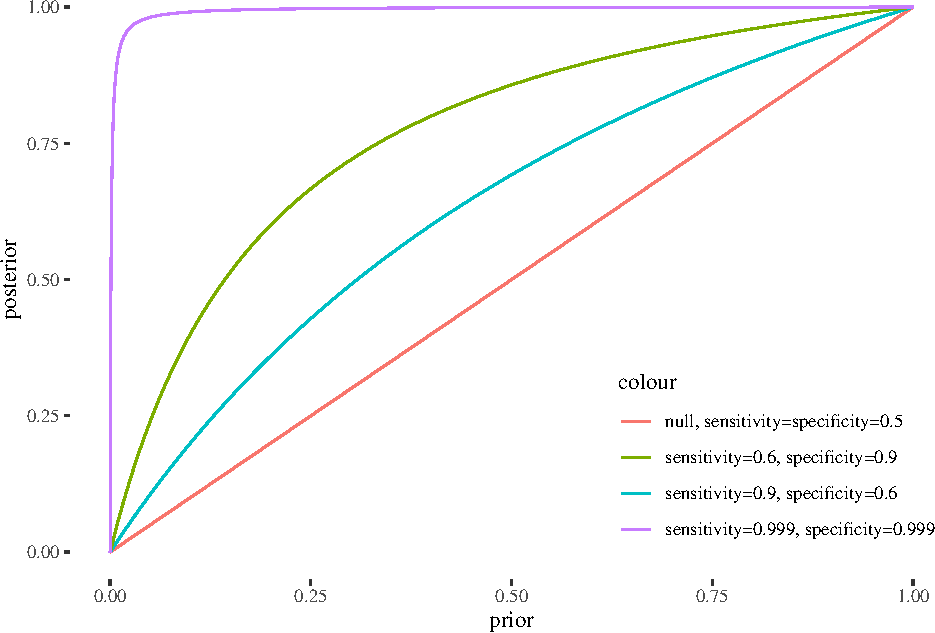
\includegraphics[width=0.9\linewidth]{conjunction-paradox2_files/figure-latex/unnamed-chunk-8-1} \end{center}

\caption{The further away the posterior line from the base 
line, the stronger the evidence irrespective 
of the prior probability of the hypothesis.}
\label{fig:strength-prior-post}
\end{figure}

\begin{figure}


\begin{center}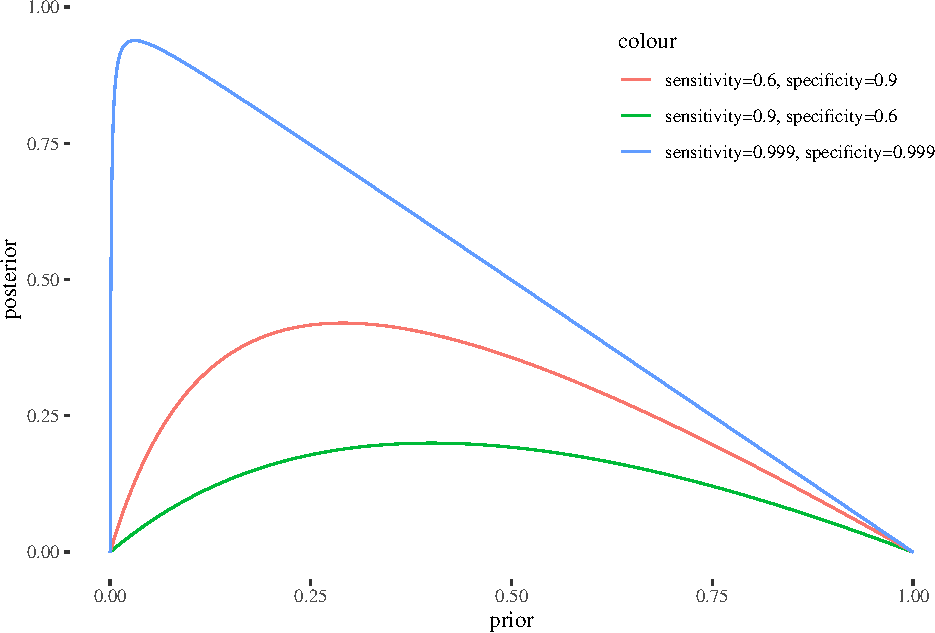
\includegraphics[width=0.9\linewidth]{conjunction-paradox2_files/figure-latex/unnamed-chunk-9-1} \end{center}

\caption{Difference between priors and posteriors as a measure of te strength of evidence.}
\label{fig:strength-difference}

\end{figure}

The same approach can model the joint evidential strength of two items
of evidence, \(a \wedge b\), relative to the combined hypothesis,
\(A \wedge B\). For simplicity, assume \(a\) and \(b\) are independent
lines of evidence supporting their respective hypothesis \(A\) and
\(B\). Further, assume \(A\) and \(B\) are probabilistically independent
of the other, as in the Bayesian network in Figure
\ref{network-conjunction} (top). The graph in Figure
\ref{fig:post-indiv-joint} (top) shows how the prior probabilities are
impacted by evidence in support of a single hypothesis---say
\(a\wedge b\) supports
\(A\)\footnote{Given the assumptions of independence we are working with, the strength of $a$ in support of $A$ is the same the strength of 
$a\wedge b$ in support of $A$ since $\frac{\pr{a\wedge b \vert A}}{\pr{a \wedge b}}$ $=\frac{\pr{a \vert A}\pr{b \vert A}}{\pr{a}\pr{b}}=\frac{\pr{a \vert A}}{\pr{a}}$.}---versus
evidence in support of a joint hypothesis---say \(a\wedge b\) supports
\(A \wedge B\). The base line is lower in the latter than in the former
case because the prior probability of \(A \wedge B\) is lower than the
prior probability of \(A\). The prior of \(A\) equals \(x\) and the
prior of \(A\wedge B\) equals \(x^2\) (assuming \(A\) and \(B\) have the
same prior probability, and as noted before, are probabilistically
independent of one another).

\begin{figure}


\begin{center}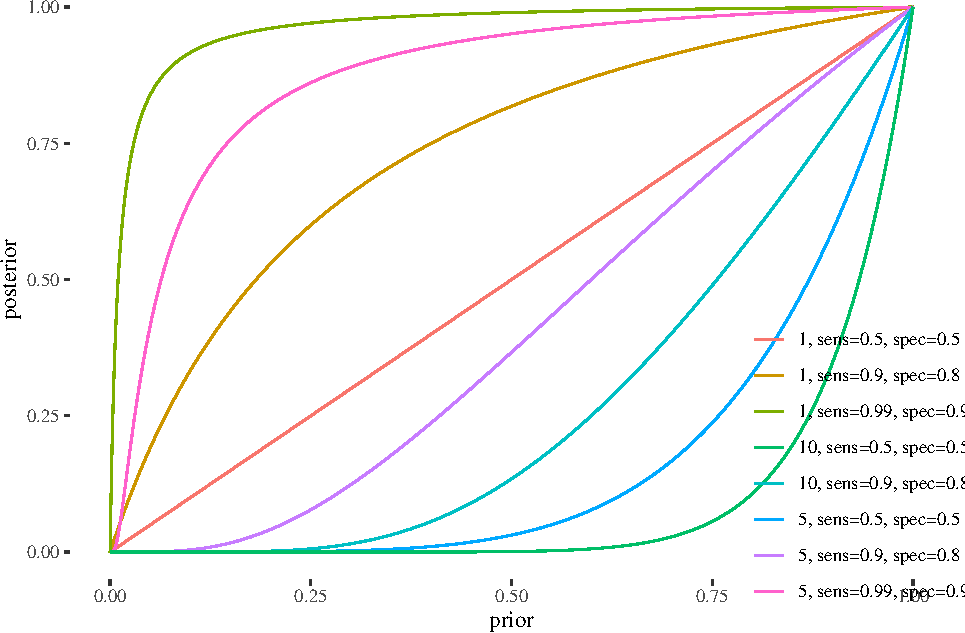
\includegraphics[width=0.9\linewidth]{conjunction-paradox2_files/figure-latex/unnamed-chunk-10-1} \end{center}




\begin{center}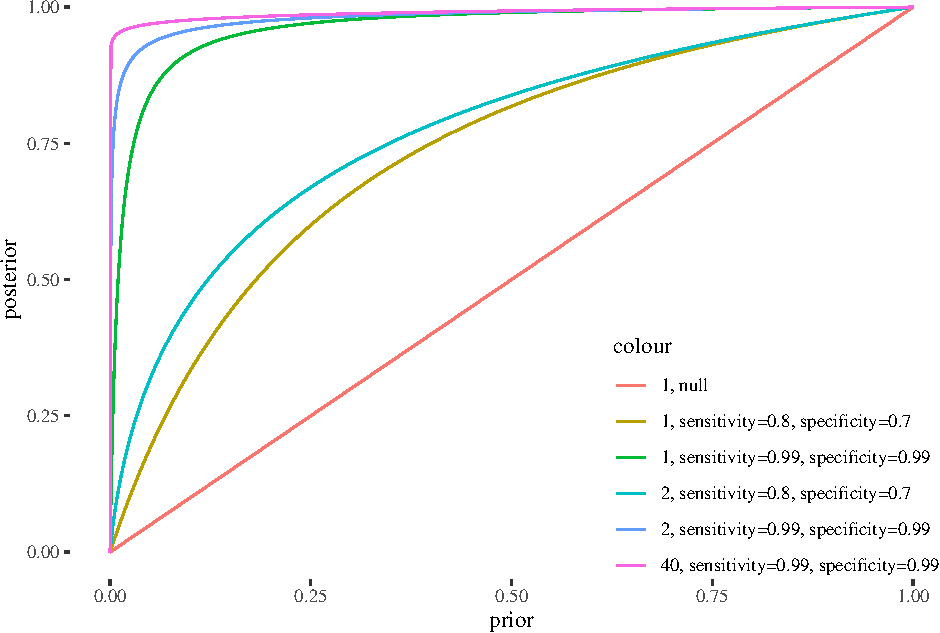
\includegraphics[width=0.9\linewidth]{conjunction-paradox2_files/figure-latex/unnamed-chunk-11-1} \end{center}

\caption{The comparison is between individual support (marked by 1, for one individual 
hypothesis) and joint support (marked by 2, for a two-claim composite claim). 
Top graph: The base line for joint support ($y=x*x$) is 
below the base line for individual support ($y=x$).
Bottom graph: the two base lines are equalized and the 
posterior lines adjusted accordingly. The posterior 
lines for individual and joint support 
get closer especially for high posterior probability values.}
\label{fig:post-indiv-joint}
\end{figure}

\begin{Shaded}
\begin{Highlighting}[]
\FunctionTok{integrate}\NormalTok{(postn, }\DecValTok{0}\NormalTok{, }\DecValTok{1}\NormalTok{, }\AttributeTok{s1 =}\FloatTok{0.99}\NormalTok{ , }\AttributeTok{s2 =}\FloatTok{0.99}\NormalTok{, }\AttributeTok{n =} \DecValTok{1}\NormalTok{)}\SpecialCharTok{$}\NormalTok{val }
\end{Highlighting}
\end{Shaded}

\begin{verbatim}
## [1] 0.9628366
\end{verbatim}

\begin{Shaded}
\begin{Highlighting}[]
\FunctionTok{integrate}\NormalTok{(postn, }\DecValTok{0}\NormalTok{, }\DecValTok{1}\NormalTok{, }\AttributeTok{s1 =}\FloatTok{0.99}\NormalTok{ , }\AttributeTok{s2 =}\FloatTok{0.99}\NormalTok{, }\AttributeTok{n =} \DecValTok{2}\NormalTok{)}\SpecialCharTok{$}\NormalTok{val }
\end{Highlighting}
\end{Shaded}

\begin{verbatim}
## [1] 0.9815782
\end{verbatim}

\begin{Shaded}
\begin{Highlighting}[]
\FunctionTok{integrate}\NormalTok{(postn, }\DecValTok{0}\NormalTok{, }\DecValTok{1}\NormalTok{, }\AttributeTok{s1 =}\FloatTok{0.99}\NormalTok{ , }\AttributeTok{s2 =}\FloatTok{0.99}\NormalTok{, }\AttributeTok{n =} \DecValTok{5}\NormalTok{)}\SpecialCharTok{$}\NormalTok{val }
\end{Highlighting}
\end{Shaded}

\begin{verbatim}
## [1] 0.9876204
\end{verbatim}

\begin{Shaded}
\begin{Highlighting}[]
\FunctionTok{integrate}\NormalTok{(postn, }\DecValTok{0}\NormalTok{, }\DecValTok{1}\NormalTok{, }\AttributeTok{s1 =}\FloatTok{0.99}\NormalTok{ , }\AttributeTok{s2 =}\FloatTok{0.99}\NormalTok{, }\AttributeTok{n =} \DecValTok{10}\NormalTok{)}\SpecialCharTok{$}\NormalTok{val}
\end{Highlighting}
\end{Shaded}

\begin{verbatim}
## [1] 0.9889299
\end{verbatim}

\begin{Shaded}
\begin{Highlighting}[]
\FunctionTok{integrate}\NormalTok{(postn, }\DecValTok{0}\NormalTok{, }\DecValTok{1}\NormalTok{, }\AttributeTok{s1 =}\FloatTok{0.99}\NormalTok{ , }\AttributeTok{s2 =}\FloatTok{0.99}\NormalTok{, }\AttributeTok{n =} \DecValTok{20}\NormalTok{)}\SpecialCharTok{$}\NormalTok{val}
\end{Highlighting}
\end{Shaded}

\begin{verbatim}
## [1] 0.989491
\end{verbatim}

\begin{Shaded}
\begin{Highlighting}[]
\FunctionTok{integrate}\NormalTok{(postn, }\DecValTok{0}\NormalTok{, }\DecValTok{1}\NormalTok{, }\AttributeTok{s1 =}\FloatTok{0.5}\NormalTok{ , }\AttributeTok{s2 =}\FloatTok{0.5}\NormalTok{, }\AttributeTok{n =} \DecValTok{1}\NormalTok{)}\SpecialCharTok{$}\NormalTok{val }
\end{Highlighting}
\end{Shaded}

\begin{verbatim}
## [1] 0.5
\end{verbatim}

\begin{Shaded}
\begin{Highlighting}[]
\FunctionTok{integrate}\NormalTok{(postn, }\DecValTok{0}\NormalTok{, }\DecValTok{1}\NormalTok{, }\AttributeTok{s1 =}\FloatTok{0.5}\NormalTok{ , }\AttributeTok{s2 =}\FloatTok{0.5}\NormalTok{, }\AttributeTok{n =} \DecValTok{2}\NormalTok{)}\SpecialCharTok{$}\NormalTok{val }
\end{Highlighting}
\end{Shaded}

\begin{verbatim}
## [1] 0.5
\end{verbatim}

\begin{Shaded}
\begin{Highlighting}[]
\FunctionTok{integrate}\NormalTok{(postn, }\DecValTok{0}\NormalTok{, }\DecValTok{1}\NormalTok{, }\AttributeTok{s1 =}\FloatTok{0.5}\NormalTok{ , }\AttributeTok{s2 =}\FloatTok{0.5}\NormalTok{, }\AttributeTok{n =} \DecValTok{5}\NormalTok{)}\SpecialCharTok{$}\NormalTok{val }
\end{Highlighting}
\end{Shaded}

\begin{verbatim}
## [1] 0.5
\end{verbatim}

\begin{Shaded}
\begin{Highlighting}[]
\FunctionTok{integrate}\NormalTok{(postn, }\DecValTok{0}\NormalTok{, }\DecValTok{1}\NormalTok{, }\AttributeTok{s1 =}\FloatTok{0.5}\NormalTok{ , }\AttributeTok{s2 =}\FloatTok{0.5}\NormalTok{, }\AttributeTok{n =} \DecValTok{10}\NormalTok{)}\SpecialCharTok{$}\NormalTok{val}
\end{Highlighting}
\end{Shaded}

\begin{verbatim}
## [1] 0.5
\end{verbatim}

\begin{Shaded}
\begin{Highlighting}[]
\FunctionTok{integrate}\NormalTok{(postn, }\DecValTok{0}\NormalTok{, }\DecValTok{1}\NormalTok{, }\AttributeTok{s1 =}\FloatTok{0.5}\NormalTok{ , }\AttributeTok{s2 =}\FloatTok{0.5}\NormalTok{, }\AttributeTok{n =} \DecValTok{20}\NormalTok{)}\SpecialCharTok{$}\NormalTok{val }
\end{Highlighting}
\end{Shaded}

\begin{verbatim}
## [1] 0.5
\end{verbatim}

\begin{Shaded}
\begin{Highlighting}[]
\FunctionTok{integrate}\NormalTok{(postn, }\DecValTok{0}\NormalTok{, }\DecValTok{1}\NormalTok{, }\AttributeTok{s1 =}\FloatTok{0.99}\NormalTok{ , }\AttributeTok{s2 =}\FloatTok{0.99}\NormalTok{, }\AttributeTok{n =} \DecValTok{1}\NormalTok{)}\SpecialCharTok{$}\NormalTok{val }\SpecialCharTok{{-}} \FunctionTok{integrate}\NormalTok{(postn, }\DecValTok{0}\NormalTok{, }\DecValTok{1}\NormalTok{, }\AttributeTok{s1 =}\FloatTok{0.5}\NormalTok{ , }\AttributeTok{s2 =}\FloatTok{0.5}\NormalTok{, }\AttributeTok{n =} \DecValTok{1}\NormalTok{)}\SpecialCharTok{$}\NormalTok{val }
\end{Highlighting}
\end{Shaded}

\begin{verbatim}
## [1] 0.4628366
\end{verbatim}

\begin{Shaded}
\begin{Highlighting}[]
\FunctionTok{integrate}\NormalTok{(postn, }\DecValTok{0}\NormalTok{, }\DecValTok{1}\NormalTok{, }\AttributeTok{s1 =}\FloatTok{0.99}\NormalTok{ , }\AttributeTok{s2 =}\FloatTok{0.99}\NormalTok{, }\AttributeTok{n =} \DecValTok{2}\NormalTok{)}\SpecialCharTok{$}\NormalTok{val }\SpecialCharTok{{-}} \FunctionTok{integrate}\NormalTok{(postn, }\DecValTok{0}\NormalTok{, }\DecValTok{1}\NormalTok{, }\AttributeTok{s1 =}\FloatTok{0.5}\NormalTok{ , }\AttributeTok{s2 =}\FloatTok{0.5}\NormalTok{, }\AttributeTok{n =} \DecValTok{2}\NormalTok{)}\SpecialCharTok{$}\NormalTok{val }
\end{Highlighting}
\end{Shaded}

\begin{verbatim}
## [1] 0.4815782
\end{verbatim}

\begin{Shaded}
\begin{Highlighting}[]
\FunctionTok{integrate}\NormalTok{(postn, }\DecValTok{0}\NormalTok{, }\DecValTok{1}\NormalTok{, }\AttributeTok{s1 =}\FloatTok{0.99}\NormalTok{ , }\AttributeTok{s2 =}\FloatTok{0.99}\NormalTok{, }\AttributeTok{n =} \DecValTok{5}\NormalTok{)}\SpecialCharTok{$}\NormalTok{val }\SpecialCharTok{{-}} \FunctionTok{integrate}\NormalTok{(postn, }\DecValTok{0}\NormalTok{, }\DecValTok{1}\NormalTok{, }\AttributeTok{s1 =}\FloatTok{0.5}\NormalTok{ , }\AttributeTok{s2 =}\FloatTok{0.5}\NormalTok{, }\AttributeTok{n =} \DecValTok{5}\NormalTok{)}\SpecialCharTok{$}\NormalTok{val }
\end{Highlighting}
\end{Shaded}

\begin{verbatim}
## [1] 0.4876204
\end{verbatim}

\begin{Shaded}
\begin{Highlighting}[]
\FunctionTok{integrate}\NormalTok{(postn, }\DecValTok{0}\NormalTok{, }\DecValTok{1}\NormalTok{, }\AttributeTok{s1 =}\FloatTok{0.99}\NormalTok{ , }\AttributeTok{s2 =}\FloatTok{0.99}\NormalTok{, }\AttributeTok{n =} \DecValTok{10}\NormalTok{)}\SpecialCharTok{$}\NormalTok{val }\SpecialCharTok{{-}} \FunctionTok{integrate}\NormalTok{(postn, }\DecValTok{0}\NormalTok{, }\DecValTok{1}\NormalTok{, }\AttributeTok{s1 =}\FloatTok{0.5}\NormalTok{ , }\AttributeTok{s2 =}\FloatTok{0.5}\NormalTok{, }\AttributeTok{n =} \DecValTok{10}\NormalTok{)}\SpecialCharTok{$}\NormalTok{val }
\end{Highlighting}
\end{Shaded}

\begin{verbatim}
## [1] 0.4889299
\end{verbatim}

\begin{Shaded}
\begin{Highlighting}[]
\FunctionTok{integrate}\NormalTok{(postn, }\DecValTok{0}\NormalTok{, }\DecValTok{1}\NormalTok{, }\AttributeTok{s1 =}\FloatTok{0.99}\NormalTok{ , }\AttributeTok{s2 =}\FloatTok{0.99}\NormalTok{, }\AttributeTok{n =} \DecValTok{20}\NormalTok{)}\SpecialCharTok{$}\NormalTok{val }\SpecialCharTok{{-}} \FunctionTok{integrate}\NormalTok{(postn, }\DecValTok{0}\NormalTok{, }\DecValTok{1}\NormalTok{, }\AttributeTok{s1 =}\FloatTok{0.5}\NormalTok{ , }\AttributeTok{s2 =}\FloatTok{0.5}\NormalTok{, }\AttributeTok{n =} \DecValTok{20}\NormalTok{)}\SpecialCharTok{$}\NormalTok{val }
\end{Highlighting}
\end{Shaded}

\begin{verbatim}
## [1] 0.489491
\end{verbatim}

\begin{Shaded}
\begin{Highlighting}[]
\FunctionTok{integrate}\NormalTok{(postn, }\DecValTok{0}\NormalTok{, }\DecValTok{1}\NormalTok{, }\AttributeTok{s1 =}\FloatTok{0.99}\NormalTok{ , }\AttributeTok{s2 =}\FloatTok{0.99}\NormalTok{, }\AttributeTok{n =} \DecValTok{25}\NormalTok{)}\SpecialCharTok{$}\NormalTok{val }\SpecialCharTok{{-}} \FunctionTok{integrate}\NormalTok{(postn, }\DecValTok{0}\NormalTok{, }\DecValTok{1}\NormalTok{, }\AttributeTok{s1 =}\FloatTok{0.5}\NormalTok{ , }\AttributeTok{s2 =}\FloatTok{0.5}\NormalTok{, }\AttributeTok{n =} \DecValTok{25}\NormalTok{)}\SpecialCharTok{$}\NormalTok{val }
\end{Highlighting}
\end{Shaded}

\begin{verbatim}
## [1] 0.4895968
\end{verbatim}

\begin{Shaded}
\begin{Highlighting}[]
\FunctionTok{integrate}\NormalTok{(postn, }\DecValTok{0}\NormalTok{, }\DecValTok{1}\NormalTok{, }\AttributeTok{s1 =}\FloatTok{0.99}\NormalTok{ , }\AttributeTok{s2 =}\FloatTok{0.99}\NormalTok{, }\AttributeTok{n =} \DecValTok{40}\NormalTok{)}\SpecialCharTok{$}\NormalTok{val }\SpecialCharTok{{-}} \FunctionTok{integrate}\NormalTok{(postn, }\DecValTok{0}\NormalTok{, }\DecValTok{1}\NormalTok{, }\AttributeTok{s1 =}\FloatTok{0.5}\NormalTok{ , }\AttributeTok{s2 =}\FloatTok{0.5}\NormalTok{, }\AttributeTok{n =} \DecValTok{40}\NormalTok{)}\SpecialCharTok{$}\NormalTok{val }
\end{Highlighting}
\end{Shaded}

\begin{verbatim}
## [1] 0.4897516
\end{verbatim}

\begin{Shaded}
\begin{Highlighting}[]
\FunctionTok{integrate}\NormalTok{(postn, }\DecValTok{0}\NormalTok{, }\DecValTok{1}\NormalTok{, }\AttributeTok{s1 =}\FloatTok{0.6}\NormalTok{ , }\AttributeTok{s2 =}\FloatTok{0.7}\NormalTok{, }\AttributeTok{n =} \DecValTok{1}\NormalTok{)}\SpecialCharTok{$}\NormalTok{val }
\end{Highlighting}
\end{Shaded}

\begin{verbatim}
## [1] 0.6137056
\end{verbatim}

\begin{Shaded}
\begin{Highlighting}[]
\FunctionTok{integrate}\NormalTok{(postn, }\DecValTok{0}\NormalTok{, }\DecValTok{1}\NormalTok{, }\AttributeTok{s1 =}\FloatTok{0.6}\NormalTok{ , }\AttributeTok{s2 =}\FloatTok{0.7}\NormalTok{, }\AttributeTok{n =} \DecValTok{2}\NormalTok{)}\SpecialCharTok{$}\NormalTok{val }
\end{Highlighting}
\end{Shaded}

\begin{verbatim}
## [1] 0.6355324
\end{verbatim}

\begin{Shaded}
\begin{Highlighting}[]
\FunctionTok{integrate}\NormalTok{(postn, }\DecValTok{0}\NormalTok{, }\DecValTok{1}\NormalTok{, }\AttributeTok{s1 =}\FloatTok{0.6}\NormalTok{ , }\AttributeTok{s2 =}\FloatTok{0.7}\NormalTok{, }\AttributeTok{n =} \DecValTok{5}\NormalTok{)}\SpecialCharTok{$}\NormalTok{val }
\end{Highlighting}
\end{Shaded}

\begin{verbatim}
## [1] 0.65284
\end{verbatim}

\begin{Shaded}
\begin{Highlighting}[]
\FunctionTok{integrate}\NormalTok{(postn, }\DecValTok{0}\NormalTok{, }\DecValTok{1}\NormalTok{, }\AttributeTok{s1 =}\FloatTok{0.6}\NormalTok{ , }\AttributeTok{s2 =}\FloatTok{0.7}\NormalTok{, }\AttributeTok{n =} \DecValTok{10}\NormalTok{)}\SpecialCharTok{$}\NormalTok{val}
\end{Highlighting}
\end{Shaded}

\begin{verbatim}
## [1] 0.6595075
\end{verbatim}

\begin{Shaded}
\begin{Highlighting}[]
\FunctionTok{integrate}\NormalTok{(postn, }\DecValTok{0}\NormalTok{, }\DecValTok{1}\NormalTok{, }\AttributeTok{s1 =}\FloatTok{0.6}\NormalTok{ , }\AttributeTok{s2 =}\FloatTok{0.7}\NormalTok{, }\AttributeTok{n =} \DecValTok{20}\NormalTok{)}\SpecialCharTok{$}\NormalTok{val}
\end{Highlighting}
\end{Shaded}

\begin{verbatim}
## [1] 0.663025
\end{verbatim}

\begin{Shaded}
\begin{Highlighting}[]
\FunctionTok{integrate}\NormalTok{(postn, }\DecValTok{0}\NormalTok{, }\DecValTok{1}\NormalTok{, }\AttributeTok{s1 =}\FloatTok{0.5}\NormalTok{ , }\AttributeTok{s2 =}\FloatTok{0.5}\NormalTok{, }\AttributeTok{n =} \DecValTok{1}\NormalTok{)}\SpecialCharTok{$}\NormalTok{val }
\end{Highlighting}
\end{Shaded}

\begin{verbatim}
## [1] 0.5
\end{verbatim}

\begin{Shaded}
\begin{Highlighting}[]
\FunctionTok{integrate}\NormalTok{(postn, }\DecValTok{0}\NormalTok{, }\DecValTok{1}\NormalTok{, }\AttributeTok{s1 =}\FloatTok{0.5}\NormalTok{ , }\AttributeTok{s2 =}\FloatTok{0.5}\NormalTok{, }\AttributeTok{n =} \DecValTok{2}\NormalTok{)}\SpecialCharTok{$}\NormalTok{val }
\end{Highlighting}
\end{Shaded}

\begin{verbatim}
## [1] 0.5
\end{verbatim}

\begin{Shaded}
\begin{Highlighting}[]
\FunctionTok{integrate}\NormalTok{(postn, }\DecValTok{0}\NormalTok{, }\DecValTok{1}\NormalTok{, }\AttributeTok{s1 =}\FloatTok{0.5}\NormalTok{ , }\AttributeTok{s2 =}\FloatTok{0.5}\NormalTok{, }\AttributeTok{n =} \DecValTok{5}\NormalTok{)}\SpecialCharTok{$}\NormalTok{val }
\end{Highlighting}
\end{Shaded}

\begin{verbatim}
## [1] 0.5
\end{verbatim}

\begin{Shaded}
\begin{Highlighting}[]
\FunctionTok{integrate}\NormalTok{(postn, }\DecValTok{0}\NormalTok{, }\DecValTok{1}\NormalTok{, }\AttributeTok{s1 =}\FloatTok{0.5}\NormalTok{ , }\AttributeTok{s2 =}\FloatTok{0.5}\NormalTok{, }\AttributeTok{n =} \DecValTok{10}\NormalTok{)}\SpecialCharTok{$}\NormalTok{val}
\end{Highlighting}
\end{Shaded}

\begin{verbatim}
## [1] 0.5
\end{verbatim}

\begin{Shaded}
\begin{Highlighting}[]
\FunctionTok{integrate}\NormalTok{(postn, }\DecValTok{0}\NormalTok{, }\DecValTok{1}\NormalTok{, }\AttributeTok{s1 =}\FloatTok{0.5}\NormalTok{ , }\AttributeTok{s2 =}\FloatTok{0.5}\NormalTok{, }\AttributeTok{n =} \DecValTok{20}\NormalTok{)}\SpecialCharTok{$}\NormalTok{val }
\end{Highlighting}
\end{Shaded}

\begin{verbatim}
## [1] 0.5
\end{verbatim}

\begin{Shaded}
\begin{Highlighting}[]
\FunctionTok{integrate}\NormalTok{(postn, }\DecValTok{0}\NormalTok{, }\DecValTok{1}\NormalTok{, }\AttributeTok{s1 =}\FloatTok{0.6}\NormalTok{ , }\AttributeTok{s2 =}\FloatTok{0.7}\NormalTok{, }\AttributeTok{n =} \DecValTok{1}\NormalTok{)}\SpecialCharTok{$}\NormalTok{val }\SpecialCharTok{{-}} \FunctionTok{integrate}\NormalTok{(postn, }\DecValTok{0}\NormalTok{, }\DecValTok{1}\NormalTok{, }\AttributeTok{s1 =}\FloatTok{0.5}\NormalTok{ , }\AttributeTok{s2 =}\FloatTok{0.5}\NormalTok{, }\AttributeTok{n =} \DecValTok{1}\NormalTok{)}\SpecialCharTok{$}\NormalTok{val }
\end{Highlighting}
\end{Shaded}

\begin{verbatim}
## [1] 0.1137056
\end{verbatim}

\begin{Shaded}
\begin{Highlighting}[]
\FunctionTok{integrate}\NormalTok{(postn, }\DecValTok{0}\NormalTok{, }\DecValTok{1}\NormalTok{, }\AttributeTok{s1 =}\FloatTok{0.6}\NormalTok{ , }\AttributeTok{s2 =}\FloatTok{0.7}\NormalTok{, }\AttributeTok{n =} \DecValTok{2}\NormalTok{)}\SpecialCharTok{$}\NormalTok{val }\SpecialCharTok{{-}} \FunctionTok{integrate}\NormalTok{(postn, }\DecValTok{0}\NormalTok{, }\DecValTok{1}\NormalTok{, }\AttributeTok{s1 =}\FloatTok{0.5}\NormalTok{ , }\AttributeTok{s2 =}\FloatTok{0.5}\NormalTok{, }\AttributeTok{n =} \DecValTok{2}\NormalTok{)}\SpecialCharTok{$}\NormalTok{val }
\end{Highlighting}
\end{Shaded}

\begin{verbatim}
## [1] 0.1355324
\end{verbatim}

\begin{Shaded}
\begin{Highlighting}[]
\FunctionTok{integrate}\NormalTok{(postn, }\DecValTok{0}\NormalTok{, }\DecValTok{1}\NormalTok{, }\AttributeTok{s1 =}\FloatTok{0.6}\NormalTok{ , }\AttributeTok{s2 =}\FloatTok{0.7}\NormalTok{, }\AttributeTok{n =} \DecValTok{5}\NormalTok{)}\SpecialCharTok{$}\NormalTok{val }\SpecialCharTok{{-}} \FunctionTok{integrate}\NormalTok{(postn, }\DecValTok{0}\NormalTok{, }\DecValTok{1}\NormalTok{, }\AttributeTok{s1 =}\FloatTok{0.5}\NormalTok{ , }\AttributeTok{s2 =}\FloatTok{0.5}\NormalTok{, }\AttributeTok{n =} \DecValTok{5}\NormalTok{)}\SpecialCharTok{$}\NormalTok{val }
\end{Highlighting}
\end{Shaded}

\begin{verbatim}
## [1] 0.15284
\end{verbatim}

\begin{Shaded}
\begin{Highlighting}[]
\FunctionTok{integrate}\NormalTok{(postn, }\DecValTok{0}\NormalTok{, }\DecValTok{1}\NormalTok{, }\AttributeTok{s1 =}\FloatTok{0.6}\NormalTok{ , }\AttributeTok{s2 =}\FloatTok{0.7}\NormalTok{, }\AttributeTok{n =} \DecValTok{10}\NormalTok{)}\SpecialCharTok{$}\NormalTok{val }\SpecialCharTok{{-}} \FunctionTok{integrate}\NormalTok{(postn, }\DecValTok{0}\NormalTok{, }\DecValTok{1}\NormalTok{, }\AttributeTok{s1 =}\FloatTok{0.5}\NormalTok{ , }\AttributeTok{s2 =}\FloatTok{0.5}\NormalTok{, }\AttributeTok{n =} \DecValTok{10}\NormalTok{)}\SpecialCharTok{$}\NormalTok{val }
\end{Highlighting}
\end{Shaded}

\begin{verbatim}
## [1] 0.1595075
\end{verbatim}

\begin{Shaded}
\begin{Highlighting}[]
\FunctionTok{integrate}\NormalTok{(postn, }\DecValTok{0}\NormalTok{, }\DecValTok{1}\NormalTok{, }\AttributeTok{s1 =}\FloatTok{0.6}\NormalTok{ , }\AttributeTok{s2 =}\FloatTok{0.7}\NormalTok{, }\AttributeTok{n =} \DecValTok{20}\NormalTok{)}\SpecialCharTok{$}\NormalTok{val }\SpecialCharTok{{-}} \FunctionTok{integrate}\NormalTok{(postn, }\DecValTok{0}\NormalTok{, }\DecValTok{1}\NormalTok{, }\AttributeTok{s1 =}\FloatTok{0.5}\NormalTok{ , }\AttributeTok{s2 =}\FloatTok{0.5}\NormalTok{, }\AttributeTok{n =} \DecValTok{20}\NormalTok{)}\SpecialCharTok{$}\NormalTok{val }
\end{Highlighting}
\end{Shaded}

\begin{verbatim}
## [1] 0.163025
\end{verbatim}

\begin{Shaded}
\begin{Highlighting}[]
\FunctionTok{integrate}\NormalTok{(postn, }\DecValTok{0}\NormalTok{, }\DecValTok{1}\NormalTok{, }\AttributeTok{s1 =}\FloatTok{0.9}\NormalTok{ , }\AttributeTok{s2 =}\FloatTok{0.8}\NormalTok{, }\AttributeTok{n =} \DecValTok{1}\NormalTok{)}\SpecialCharTok{$}\NormalTok{val }
\end{Highlighting}
\end{Shaded}

\begin{verbatim}
## [1] 0.7331961
\end{verbatim}

\begin{Shaded}
\begin{Highlighting}[]
\FunctionTok{integrate}\NormalTok{(postn, }\DecValTok{0}\NormalTok{, }\DecValTok{1}\NormalTok{, }\AttributeTok{s1 =}\FloatTok{0.9}\NormalTok{ , }\AttributeTok{s2 =}\FloatTok{0.8}\NormalTok{, }\AttributeTok{n =} \DecValTok{2}\NormalTok{)}\SpecialCharTok{$}\NormalTok{val }
\end{Highlighting}
\end{Shaded}

\begin{verbatim}
## [1] 0.7717311
\end{verbatim}

\begin{Shaded}
\begin{Highlighting}[]
\FunctionTok{integrate}\NormalTok{(postn, }\DecValTok{0}\NormalTok{, }\DecValTok{1}\NormalTok{, }\AttributeTok{s1 =}\FloatTok{0.9}\NormalTok{ , }\AttributeTok{s2 =}\FloatTok{0.8}\NormalTok{, }\AttributeTok{n =} \DecValTok{5}\NormalTok{)}\SpecialCharTok{$}\NormalTok{val }
\end{Highlighting}
\end{Shaded}

\begin{verbatim}
## [1] 0.7990992
\end{verbatim}

\begin{Shaded}
\begin{Highlighting}[]
\FunctionTok{integrate}\NormalTok{(postn, }\DecValTok{0}\NormalTok{, }\DecValTok{1}\NormalTok{, }\AttributeTok{s1 =}\FloatTok{0.9}\NormalTok{ , }\AttributeTok{s2 =}\FloatTok{0.8}\NormalTok{, }\AttributeTok{n =} \DecValTok{10}\NormalTok{)}\SpecialCharTok{$}\NormalTok{val}
\end{Highlighting}
\end{Shaded}

\begin{verbatim}
## [1] 0.8086466
\end{verbatim}

\begin{Shaded}
\begin{Highlighting}[]
\FunctionTok{integrate}\NormalTok{(postn, }\DecValTok{0}\NormalTok{, }\DecValTok{1}\NormalTok{, }\AttributeTok{s1 =}\FloatTok{0.9}\NormalTok{ , }\AttributeTok{s2 =}\FloatTok{0.8}\NormalTok{, }\AttributeTok{n =} \DecValTok{20}\NormalTok{)}\SpecialCharTok{$}\NormalTok{val}
\end{Highlighting}
\end{Shaded}

\begin{verbatim}
## [1] 0.8134273
\end{verbatim}

\begin{Shaded}
\begin{Highlighting}[]
\FunctionTok{integrate}\NormalTok{(postn, }\DecValTok{0}\NormalTok{, }\DecValTok{1}\NormalTok{, }\AttributeTok{s1 =}\FloatTok{0.5}\NormalTok{ , }\AttributeTok{s2 =}\FloatTok{0.5}\NormalTok{, }\AttributeTok{n =} \DecValTok{1}\NormalTok{)}\SpecialCharTok{$}\NormalTok{val }
\end{Highlighting}
\end{Shaded}

\begin{verbatim}
## [1] 0.5
\end{verbatim}

\begin{Shaded}
\begin{Highlighting}[]
\FunctionTok{integrate}\NormalTok{(postn, }\DecValTok{0}\NormalTok{, }\DecValTok{1}\NormalTok{, }\AttributeTok{s1 =}\FloatTok{0.5}\NormalTok{ , }\AttributeTok{s2 =}\FloatTok{0.5}\NormalTok{, }\AttributeTok{n =} \DecValTok{2}\NormalTok{)}\SpecialCharTok{$}\NormalTok{val }
\end{Highlighting}
\end{Shaded}

\begin{verbatim}
## [1] 0.5
\end{verbatim}

\begin{Shaded}
\begin{Highlighting}[]
\FunctionTok{integrate}\NormalTok{(postn, }\DecValTok{0}\NormalTok{, }\DecValTok{1}\NormalTok{, }\AttributeTok{s1 =}\FloatTok{0.5}\NormalTok{ , }\AttributeTok{s2 =}\FloatTok{0.5}\NormalTok{, }\AttributeTok{n =} \DecValTok{5}\NormalTok{)}\SpecialCharTok{$}\NormalTok{val }
\end{Highlighting}
\end{Shaded}

\begin{verbatim}
## [1] 0.5
\end{verbatim}

\begin{Shaded}
\begin{Highlighting}[]
\FunctionTok{integrate}\NormalTok{(postn, }\DecValTok{0}\NormalTok{, }\DecValTok{1}\NormalTok{, }\AttributeTok{s1 =}\FloatTok{0.5}\NormalTok{ , }\AttributeTok{s2 =}\FloatTok{0.5}\NormalTok{, }\AttributeTok{n =} \DecValTok{10}\NormalTok{)}\SpecialCharTok{$}\NormalTok{val}
\end{Highlighting}
\end{Shaded}

\begin{verbatim}
## [1] 0.5
\end{verbatim}

\begin{Shaded}
\begin{Highlighting}[]
\FunctionTok{integrate}\NormalTok{(postn, }\DecValTok{0}\NormalTok{, }\DecValTok{1}\NormalTok{, }\AttributeTok{s1 =}\FloatTok{0.5}\NormalTok{ , }\AttributeTok{s2 =}\FloatTok{0.5}\NormalTok{, }\AttributeTok{n =} \DecValTok{20}\NormalTok{)}\SpecialCharTok{$}\NormalTok{val }
\end{Highlighting}
\end{Shaded}

\begin{verbatim}
## [1] 0.5
\end{verbatim}

\begin{Shaded}
\begin{Highlighting}[]
\FunctionTok{integrate}\NormalTok{(postn, }\DecValTok{0}\NormalTok{, }\DecValTok{1}\NormalTok{, }\AttributeTok{s1 =}\FloatTok{0.9}\NormalTok{ , }\AttributeTok{s2 =}\FloatTok{0.8}\NormalTok{, }\AttributeTok{n =} \DecValTok{1}\NormalTok{)}\SpecialCharTok{$}\NormalTok{val }\SpecialCharTok{{-}} \FunctionTok{integrate}\NormalTok{(postn, }\DecValTok{0}\NormalTok{, }\DecValTok{1}\NormalTok{, }\AttributeTok{s1 =}\FloatTok{0.5}\NormalTok{ , }\AttributeTok{s2 =}\FloatTok{0.5}\NormalTok{, }\AttributeTok{n =} \DecValTok{1}\NormalTok{)}\SpecialCharTok{$}\NormalTok{val }
\end{Highlighting}
\end{Shaded}

\begin{verbatim}
## [1] 0.2331961
\end{verbatim}

\begin{Shaded}
\begin{Highlighting}[]
\FunctionTok{integrate}\NormalTok{(postn, }\DecValTok{0}\NormalTok{, }\DecValTok{1}\NormalTok{, }\AttributeTok{s1 =}\FloatTok{0.9}\NormalTok{ , }\AttributeTok{s2 =}\FloatTok{0.8}\NormalTok{, }\AttributeTok{n =} \DecValTok{2}\NormalTok{)}\SpecialCharTok{$}\NormalTok{val }\SpecialCharTok{{-}} \FunctionTok{integrate}\NormalTok{(postn, }\DecValTok{0}\NormalTok{, }\DecValTok{1}\NormalTok{, }\AttributeTok{s1 =}\FloatTok{0.5}\NormalTok{ , }\AttributeTok{s2 =}\FloatTok{0.5}\NormalTok{, }\AttributeTok{n =} \DecValTok{2}\NormalTok{)}\SpecialCharTok{$}\NormalTok{val }
\end{Highlighting}
\end{Shaded}

\begin{verbatim}
## [1] 0.2717311
\end{verbatim}

\begin{Shaded}
\begin{Highlighting}[]
\FunctionTok{integrate}\NormalTok{(postn, }\DecValTok{0}\NormalTok{, }\DecValTok{1}\NormalTok{, }\AttributeTok{s1 =}\FloatTok{0.9}\NormalTok{ , }\AttributeTok{s2 =}\FloatTok{0.8}\NormalTok{, }\AttributeTok{n =} \DecValTok{5}\NormalTok{)}\SpecialCharTok{$}\NormalTok{val }\SpecialCharTok{{-}} \FunctionTok{integrate}\NormalTok{(postn, }\DecValTok{0}\NormalTok{, }\DecValTok{1}\NormalTok{, }\AttributeTok{s1 =}\FloatTok{0.5}\NormalTok{ , }\AttributeTok{s2 =}\FloatTok{0.5}\NormalTok{, }\AttributeTok{n =} \DecValTok{5}\NormalTok{)}\SpecialCharTok{$}\NormalTok{val }
\end{Highlighting}
\end{Shaded}

\begin{verbatim}
## [1] 0.2990992
\end{verbatim}

\begin{Shaded}
\begin{Highlighting}[]
\FunctionTok{integrate}\NormalTok{(postn, }\DecValTok{0}\NormalTok{, }\DecValTok{1}\NormalTok{, }\AttributeTok{s1 =}\FloatTok{0.9}\NormalTok{ , }\AttributeTok{s2 =}\FloatTok{0.8}\NormalTok{, }\AttributeTok{n =} \DecValTok{10}\NormalTok{)}\SpecialCharTok{$}\NormalTok{val }\SpecialCharTok{{-}} \FunctionTok{integrate}\NormalTok{(postn, }\DecValTok{0}\NormalTok{, }\DecValTok{1}\NormalTok{, }\AttributeTok{s1 =}\FloatTok{0.5}\NormalTok{ , }\AttributeTok{s2 =}\FloatTok{0.5}\NormalTok{, }\AttributeTok{n =} \DecValTok{10}\NormalTok{)}\SpecialCharTok{$}\NormalTok{val }
\end{Highlighting}
\end{Shaded}

\begin{verbatim}
## [1] 0.3086466
\end{verbatim}

\begin{Shaded}
\begin{Highlighting}[]
\FunctionTok{integrate}\NormalTok{(postn, }\DecValTok{0}\NormalTok{, }\DecValTok{1}\NormalTok{, }\AttributeTok{s1 =}\FloatTok{0.9}\NormalTok{ , }\AttributeTok{s2 =}\FloatTok{0.8}\NormalTok{, }\AttributeTok{n =} \DecValTok{20}\NormalTok{)}\SpecialCharTok{$}\NormalTok{val }\SpecialCharTok{{-}} \FunctionTok{integrate}\NormalTok{(postn, }\DecValTok{0}\NormalTok{, }\DecValTok{1}\NormalTok{, }\AttributeTok{s1 =}\FloatTok{0.5}\NormalTok{ , }\AttributeTok{s2 =}\FloatTok{0.5}\NormalTok{, }\AttributeTok{n =} \DecValTok{20}\NormalTok{)}\SpecialCharTok{$}\NormalTok{val }
\end{Highlighting}
\end{Shaded}

\begin{verbatim}
## [1] 0.3134273
\end{verbatim}

\begin{Shaded}
\begin{Highlighting}[]
\FunctionTok{integrate}\NormalTok{(post, }\DecValTok{0}\NormalTok{, }\DecValTok{1}\NormalTok{, }\AttributeTok{s1 =}\FloatTok{0.99}\NormalTok{ , }\AttributeTok{s2 =}\FloatTok{0.99}\NormalTok{)}\SpecialCharTok{$}\NormalTok{val }
\end{Highlighting}
\end{Shaded}

\begin{verbatim}
## [1] 0.9628366
\end{verbatim}

\begin{Shaded}
\begin{Highlighting}[]
\FunctionTok{integrate}\NormalTok{(postn, }\DecValTok{0}\NormalTok{, }\DecValTok{1}\NormalTok{, }\AttributeTok{s1 =}\FloatTok{0.99}\NormalTok{ , }\AttributeTok{s2 =}\FloatTok{0.99}\NormalTok{ , }\AttributeTok{n =} \DecValTok{2}\NormalTok{)}\SpecialCharTok{$}\NormalTok{val}
\end{Highlighting}
\end{Shaded}

\begin{verbatim}
## [1] 0.9815782
\end{verbatim}

\begin{Shaded}
\begin{Highlighting}[]
\FunctionTok{integrate}\NormalTok{(postn, }\DecValTok{0}\NormalTok{, }\DecValTok{1}\NormalTok{, }\AttributeTok{s1 =}\FloatTok{0.99}\NormalTok{ , }\AttributeTok{s2 =}\FloatTok{0.99}\NormalTok{ , }\AttributeTok{n =} \DecValTok{5}\NormalTok{)}\SpecialCharTok{$}\NormalTok{val}
\end{Highlighting}
\end{Shaded}

\begin{verbatim}
## [1] 0.9876204
\end{verbatim}

\begin{figure}


\begin{center}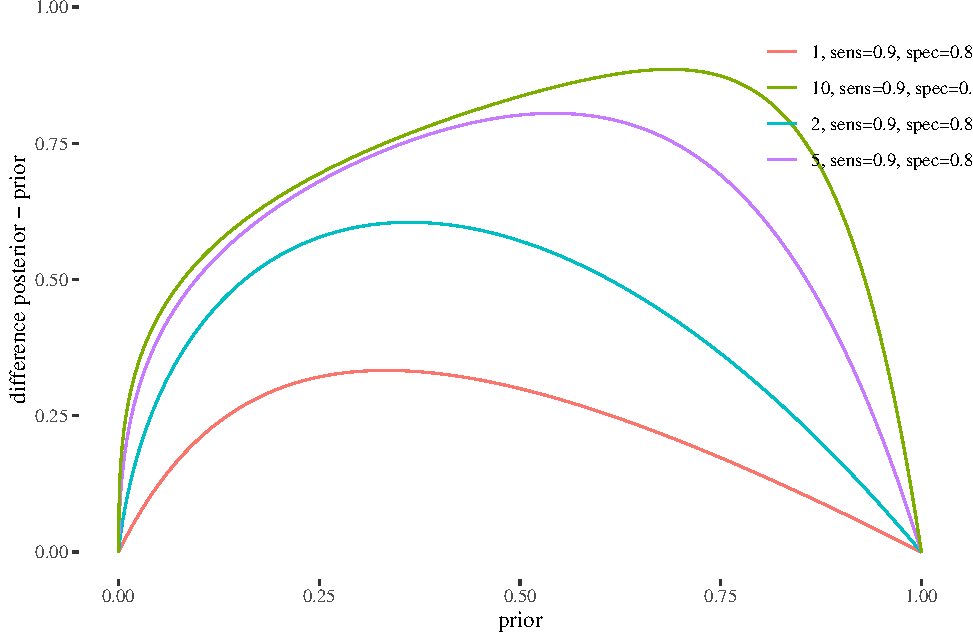
\includegraphics[width=0.9\linewidth]{conjunction-paradox2_files/figure-latex/unnamed-chunk-16-1} \end{center}


\end{figure}

\begin{Shaded}
\begin{Highlighting}[]
\NormalTok{prior\_a }\OtherTok{\textless{}{-}} \FloatTok{0.6}
\NormalTok{prior\_b }\OtherTok{\textless{}{-}} \FloatTok{0.4}
\NormalTok{sen\_a }\OtherTok{\textless{}{-}} \FloatTok{0.85}  \CommentTok{\# Pr(a given A)}
\NormalTok{spe\_a }\OtherTok{\textless{}{-}} \FloatTok{0.75}  \CommentTok{\#  Pr(not{-}a given not{-}A)}
\NormalTok{sen\_b }\OtherTok{\textless{}{-}} \FloatTok{0.7}
\NormalTok{spe\_b }\OtherTok{\textless{}{-}} \FloatTok{0.75}

\NormalTok{prior\_ab }\OtherTok{\textless{}{-}}\NormalTok{ prior\_a}\SpecialCharTok{*}\NormalTok{prior\_b }

\NormalTok{bf\_a }\OtherTok{\textless{}{-}}\NormalTok{ sen\_a}\SpecialCharTok{/}\NormalTok{((sen\_a}\SpecialCharTok{*}\NormalTok{prior\_a)}\SpecialCharTok{+}\NormalTok{((}\DecValTok{1}\SpecialCharTok{{-}}\NormalTok{spe\_a)}\SpecialCharTok{*}\NormalTok{(}\DecValTok{1}\SpecialCharTok{{-}}\NormalTok{prior\_a)))}
\NormalTok{bf\_b }\OtherTok{\textless{}{-}}\NormalTok{ sen\_b}\SpecialCharTok{/}\NormalTok{((sen\_b}\SpecialCharTok{*}\NormalTok{prior\_b)}\SpecialCharTok{+}\NormalTok{((}\DecValTok{1}\SpecialCharTok{{-}}\NormalTok{spe\_b)}\SpecialCharTok{*}\NormalTok{(}\DecValTok{1}\SpecialCharTok{{-}}\NormalTok{prior\_b)))}
\NormalTok{bf\_ab }\OtherTok{\textless{}{-}}\NormalTok{ bf\_a}\SpecialCharTok{*}\NormalTok{bf\_b}

\NormalTok{post\_a }\OtherTok{\textless{}{-}}\NormalTok{ bf\_a}\SpecialCharTok{*}\NormalTok{prior\_a}
\NormalTok{post\_b }\OtherTok{\textless{}{-}}\NormalTok{ bf\_b}\SpecialCharTok{*}\NormalTok{prior\_b}
\NormalTok{post\_ab }\OtherTok{\textless{}{-}}\NormalTok{ bf\_ab}\SpecialCharTok{*}\NormalTok{prior\_ab}

\NormalTok{prior\_a}
\end{Highlighting}
\end{Shaded}

\begin{verbatim}
## [1] 0.6
\end{verbatim}

\begin{Shaded}
\begin{Highlighting}[]
\NormalTok{prior\_b}
\end{Highlighting}
\end{Shaded}

\begin{verbatim}
## [1] 0.4
\end{verbatim}

\begin{Shaded}
\begin{Highlighting}[]
\NormalTok{prior\_ab}
\end{Highlighting}
\end{Shaded}

\begin{verbatim}
## [1] 0.24
\end{verbatim}

\begin{Shaded}
\begin{Highlighting}[]
\NormalTok{post\_a}
\end{Highlighting}
\end{Shaded}

\begin{verbatim}
## [1] 0.8360656
\end{verbatim}

\begin{Shaded}
\begin{Highlighting}[]
\NormalTok{post\_b}
\end{Highlighting}
\end{Shaded}

\begin{verbatim}
## [1] 0.6511628
\end{verbatim}

\begin{Shaded}
\begin{Highlighting}[]
\NormalTok{post\_ab}
\end{Highlighting}
\end{Shaded}

\begin{verbatim}
## [1] 0.5444148
\end{verbatim}

\begin{Shaded}
\begin{Highlighting}[]
\NormalTok{prior\_a }\OtherTok{\textless{}{-}} \FloatTok{0.24}
\NormalTok{prior\_b }\OtherTok{\textless{}{-}} \FloatTok{0.24}

\NormalTok{bf\_a }\OtherTok{\textless{}{-}}\NormalTok{ sen\_a}\SpecialCharTok{/}\NormalTok{((sen\_a}\SpecialCharTok{*}\NormalTok{prior\_a)}\SpecialCharTok{+}\NormalTok{((}\DecValTok{1}\SpecialCharTok{{-}}\NormalTok{spe\_a)}\SpecialCharTok{*}\NormalTok{(}\DecValTok{1}\SpecialCharTok{{-}}\NormalTok{prior\_a)))}
\NormalTok{bf\_b }\OtherTok{\textless{}{-}}\NormalTok{ sen\_b}\SpecialCharTok{/}\NormalTok{((sen\_b}\SpecialCharTok{*}\NormalTok{prior\_b)}\SpecialCharTok{+}\NormalTok{((}\DecValTok{1}\SpecialCharTok{{-}}\NormalTok{spe\_b)}\SpecialCharTok{*}\NormalTok{(}\DecValTok{1}\SpecialCharTok{{-}}\NormalTok{prior\_b)))}
\NormalTok{bf\_ab }\OtherTok{\textless{}{-}}\NormalTok{ bf\_a}\SpecialCharTok{*}\NormalTok{bf\_b}

\NormalTok{post\_a }\OtherTok{\textless{}{-}}\NormalTok{ bf\_a}\SpecialCharTok{*}\NormalTok{prior\_a}
\NormalTok{post\_b }\OtherTok{\textless{}{-}}\NormalTok{ bf\_b}\SpecialCharTok{*}\NormalTok{prior\_b}
\NormalTok{post\_a}
\end{Highlighting}
\end{Shaded}

\begin{verbatim}
## [1] 0.5177665
\end{verbatim}

\begin{Shaded}
\begin{Highlighting}[]
\NormalTok{post\_b}
\end{Highlighting}
\end{Shaded}

\begin{verbatim}
## [1] 0.4692737
\end{verbatim}

What happens if we make the same comparison between individual and
composite claims by equalizing their prior probability? If the claims
are independent and equiprobable, let \(x\) be the prior probability of
an individual claim (when it is considered in isolation) and let
\(x^{1/k}\) the prior probability of the same individual claim when it
is part of a composite claim that consists of \(k\) claims. In this
way---and again, assuming independence and equiprobability of the
hypotheses---the prior probability of the composite claim equals the
prior probability of the individual claim since \((x^{1/k})^k=x\), as
desired. These different claims are then plotted having the same priors.
Here we are explicitly factoring out the role of prior probabilities.
Figure \ref{fig:post-indiv-joint} (bottom) shows the result of this
process of equalization.

We observe two things. First, the difference in posterior probability,
though still present, is less significant, especially for values above
the 75\% threshold and even more clearly above the 95\% threshold.
Second, whatever remaining difference in posterior probability is now
reversed, that is, a composite claim supported by several items of
evidence has a higher posterior probability compared to an individual
claim supported by one item of evidence. This second observation agrees
with the analysis based on the Bayes factor and the likelihood ratio in
the earlier section. That analysis showed that the support for a
composite claim by a joint body of evidence often exceeds the support
for an individual claim.

These two observations establish that, by factorig out prior
probabilities and under certain independence assumptions, whenever the
individual claims meet the applicable posterior threhsold, so does the
composite claim. This verifies aggregation. Conversely, whenever the
composite claim, say \(A \wedge B\), meets the applicable posterior
threshold, so do the individual claims insofar as the threshold is about
75\% or higher. This verifies---to some approximation and in a limited
class of cases---the other direction of the conjunction principle, what
we called distribution.

Has the distribution paradox been eliminated then? The approach we have
just described---equalizing the prior probabilities across individual
and composite claims---does not entirely eliminate the paradox. There
are still cases in which a composite hypothesis, say \(A \wedge B\),
receives stronger support than an individual hypothesis, given the same
body of evidence. Sensitivity to priors seems to play a role. But it
cannot be the only factor at play, or else the equalization of the prior
probabilities would have eliminated the paradox entirely. So what else
is going on?

\hypertarget{weaker-claims-weaken-sensitivity}{%
\subsection{Weaker Claims Weaken
Sensitivity}\label{weaker-claims-weaken-sensitivity}}

Let's examine more closely the Bayes factor and the likelihood ratio as
measures of evidential strength. Likelihood ratios are comparative in
nature. Suppose we compare claim \(A\) and claim \(A\wedge B\) relative
to the same body of evidence \(a\wedge b\). Thinks of \(A\) as `the
defendant physically injured the victim' while \(B\) as `the defendant
knew the victim was a firefighter.' Think of \(a\) and \(b\) as
testimonies each supporting one of the two hypotheses. We are still
working with the Bayesian networks in Figure \ref{network-conjunction}.

Consider the combined body of evidence \(a\wedge b\). Which claim
between \(A\) and \(A\wedge B\) will receive more support by evidence
\(a\wedge b\)? Intuitively, one might think that \(A\) should receive
more or at least equal support compared to \(A\wedge B\) . After all,
\(A\wedge B\) is a stronger claim than \(A\) and thus more difficult to
establish than \(A\), other things being equal. In terms of posterior
probabilities, this is true. The posterior probability of \(A\wedge B\)
should not be higher than the posterior probability of \(A\) alone given
evidence \(a \wedge b\).

Let's now think in terms of evidential support. Formally, the question
is whether
\(\frac{\pr{a\wedge b \vert A}}{\pr{a\wedge b \vert A \wedge B}}\) is
less than one or greater than one. Given the customary independencies
between evidence and hypotheses,

\[\frac{\pr{a\wedge b \vert A}}{\pr{a\wedge b \vert A \wedge B}}=\frac{\pr{a \vert A} \pr{b \vert A}}{\pr{a \vert A} \pr{b \vert B}}=\frac{\pr{b \vert A}}{\pr{b \vert B}}<1.\]

\noindent The reason is that \(\pr{b \vert A} < \pr{b \vert B}\) since
the sensitivity of \(b\) relative to \(B\) should be higher than the
sensitivity of \(b\) relative to \(A\).\footnote{GIVE PROOF OF THIS}
This is obvious if \(A\) and \(b\) are independent claims, as in the
Bayesian networks in Figure \ref{network-conjunction} (bottom). In this
case, \(\pr{b \vert A}=\pr{b}\).\\
So \(\frac{\pr{b}}{\pr{b \vert B}}<1\) since \(b\), by assumption,
positively supports \(B\), or in other words,
\(\frac{\pr{b \vert B}}{\pr{b}}>1\). Thus, \(a\wedge b\) supports
\(A\wedge B\) more than it supports \(A\) alone. This is not what one
would expect intuitively.

The same conslusion holds using the Bayes factor. If
\(\frac{\pr{a\wedge b \vert A}}{\pr{a\wedge b \vert A \wedge B}}<1\),
then

\[\frac{\pr{a\wedge b \vert A}}{\pr{a\wedge b}} < \frac{\pr{a\wedge b \vert A \wedge B}}{\pr{a\wedge b}}   \]

\noindent Thus, evidence \(a\wedge b\) better supports, even on an
absolute scale, \(A \wedge B\) compared to \(A\). Note that, even if the
Baye factor depends on the priors, the difference here is not due to the
difference between the priors of \(A\) and the priors of \(A\wedge B\)
since the denominator is simply
\(\pr{a\wedge b}\).\footnote{Note that $\pr{a\wedge b \vert A}\pr{A}+ \pr{a\wedge b \vert \neg A}\pr\neg {A}$ is the same as $\pr{a\wedge b \vert (A\wedge B)}\pr{A\wedge B}+ \pr{a\wedge b \vert \neg (A\wedge B)}\pr{\neg (A\wedge B)}$. \textbf{NEED A PROOF FOR THIS BUT IT SHOULD HOLD, RIGHT?}}

What we have said so far agrees with the claim defended in the previous
section. That is, even when \(a\wedge b\) strongly supports
\(A \wedge B\), the same evidence need \textit{not} strongly support
\(A\). Formally,

\[\frac{\pr{a\wedge b \vert A}}{\pr{a\wedge b \vert \neg A}} < \frac{\pr{a\wedge b \vert A \wedge B}}{\pr{a\wedge b \vert \neg (A \wedge B)}}\]

\noindent In other words, even if \(a\wedge b\) favors \(A\wedge B\)
over its negation to a very high degree, it need not favor equally
strongly \(A\) over its negation. This is a comparative claim about two
compartive claims, and as such, it may not be easy to parse. Evidential
support, when it is formalized by the likelihoo ratio, is always
relative to a contrast class. In comparing the support that the same
body of evidence provides to \(A\) as contrasted to \(A\wedge B\), it
might be better to include these two hypotheses in the contrast class.
So the expression
\(\frac{\pr{a\wedge b \vert A}}{\pr{a\wedge b \vert A \wedge B}}\) is
more straightforward.

No matter the formulation, the same conclusion holds. Evidence
\(a\wedge b\) supports the composite claim \(A\wedge B\) more than it
supports the weaker claim \(A\), even assuming that \(A\) and \(B\) are
independent of one another and thus not mutually reinforcing. This
conclusion seems paradoxical. How should we make sense of it? At first,
we thought the paradox could be due to prior dependency since the
combined likelihood ratio
\(\frac{\pr{a\wedge b \vert A \wedge B}}{\pr{a\wedge b \vert \neg (A \wedge B)}}\)
varies depending on the priors of \(A\) and \(B\). But this argument
seems to no longer holds since in case of
\(\frac{\pr{a\wedge b \vert A}}{\pr{a\wedge b \vert A \wedge B}}\) any
prior dependency seems to have been eliminated. After all, if
\(\frac{\pr{a\wedge b \vert A}}{\pr{a\wedge b \vert A \wedge B}}<1\),
the sensitivity of \(a\wedge b\) must be worse relative to \(A\) than
the composite claim \(A \wedge B\).

Sensitivity is a crucial property of the quality of the evidence.
Everything else being equal, the lower the sensitivity of the evidence,
the lower its evidential strength. The importance of sensitivity as a
factor for assessing the strength of the evidence is hard to dispute. So
why is the sensitivity of \(a\wedge b\) worse relative to \(A\) than
\(A \wedge B\)? Suppose \(A\) is the case. If \(A\) is the case, in
order for \(a\wedge b\) to arise, both \(a\) and \(b\) should pick up on
\(A\). If \(b\) fails to pick up on \(A\), then \(A \wedge b\) would not
arise even if \(a\) pick up on
\(A\).\footnote{The occurrance of $a\wedge b$ is less likely to occur than just $a$ alone picking up on $A$ because $b$ may fail---and fail more often than $a$ would---in picking up on $A$.}
Suppose instead \(A\wedge B\) holds. In this case, \(a\wedge b\) would
arise even if \(b\) fails to pick up on \(A\) so long \(a\) picks up on
\(A\) and \(b\) picks up on \(B\). Now of course \(b\) could also fail
to pick on \(B\) just like \(a\) could fail to pick up on \(B\). But we
are assuming that \(b\) is better than \(a\) at tracking \(B\). So \(b\)
will fail less often than \(a\) at picking up on \(B\). Thus, the
sensitivity of \(a\wedge b\) relative to \(A\wedge B\) is better than
the sensitivity of \(a\) relative to \(A\) alone. This is a subtle point
that probability theory helps to bring out clearly.

How big are these variations?
\textbf{PLOT GRAPH TO GET A SENSE OF VARIATIONS OF SENSITIVITY}

One explanation of the paradox, then, is the difference in sensitivity.
The sensitivity of \(a\wedge b\) relative to \(A\wedge B\) is better
than the sensitivity of the same evidence relative to \(A\).
Consequently, other thigns being equal, evidence \(a\wedge b\) supports
\(A\wedge B\) better than \(A\). However counterintuitive this might
seem, we should accept this fact and admit that our intuitions were
wrong. So the fallacy seems to be to assume that the sensitivity of
\(a\wedge b\) relative to \(A\) cannot be lower than the senstivity of
\(a\wedge b\) relative to \(A\wedge B\). The thought would be something
like this: if \(a \wedge b\) tracks \(A\wedge B\) to some degree, it
surely must be able to track \(A\) alone, at least as well. But we have
just shown that we cannot assume that
\(\pr{a\wedge b \vert A} \geq \pr{a\wedge b \vert A\wedge B}\) and in
fact the opposite is the case,
\(\pr{a\wedge b \vert A} < \pr{a\wedge b \vert A\wedge B}\).

Another way to convince ourselves this is the case is to run a
simulation. Suppose we are deciding about the truth of \(A\) and the the
truth of \(A\wedge B\), and we have a fixed body of evidence, say,
\(a\wedge b\) that speaks in favor of both claims.
\todo{M: Run simulation to show that same diagnostic test for composite claim would perform better then when applied to individual claim (worse LR). How do to do this? HELP!}

We should circumscribe the point we just made since it does not always
hold. Suppose, as in Figure \ref{network-unrelated}, that \(H\) is a
claim unrelated to \(A\) and evidence \(a\). Evidence \(a\) supports
\(A\). Would the composite claim \(A\wedge H\) be better supported by
\(a\) than \(A\) alone? It would not. Mere tagging an unrelated
hypothesis does not strengthen the evidence. Note that
\(\pr{a \vert A}=\pr{a \vert A \wedge H}\) because \(H\) is indepedent
from everything else. Thus,

\[\frac{\pr{a \vert A}}{\pr{a \vert A \wedge H}}=\frac{\pr{a \vert A}}{\pr{a \vert A}}=1.\]

\noindent Tagging an unrelated claim \(H\) does not strengthen the
evidence, but leaves it unchanged. Similarly, suppose \(B\) constitutes
one element of a crime and \(A\) constitutes the other element. The two
claims are independent, each supported by items of evidence \(a\) and
\(b\) respectively. This is our standard set up. If \(a\) supports
\(A\), would \(a\) support \(A\wedge B\) more strongly than it supports
\(A\) alone? Here we no longer have \(a\wedge b\), but instead, \(a\)
alone. The question is whether
\(\frac{\pr{a \vert A}}{\pr{a \vert A \wedge B}}>1\) or
\(\frac{\pr{a \vert A}}{\pr{a \vert A \wedge B}}<1\). Given the usual
independencies between evidence and hypotheses,

\[\frac{\pr{a\vert A}}{\pr{a \vert A \wedge B}}=\frac{\pr{a \vert A}}{\pr{a \vert A}}=1\]

Evidence \(a\) supports \(A\) and \(A\wedge B\) to the same extent. One
might complain that this is counterintuitive. How can it be that \(a\)
supports \(A\) to the same degree that it supports the more demanding
claim \(A\wedge H\) or \(A\wedge B\)? For suppose we have evidence \(a\)
in favor of \(A\) and then wonder whether we could use that evidence in
support of another claim \(H\) or \(B\). By tagging \(H\) or \(B\) to
\(A\), we can at least say that we have evidence \(a\) for \(A\wedge H\)
or \(A\wedge B\) that is at least as strong as evidence \(a\) in support
of \(A\). But note that \(\frac{\pr{a \vert A}}{\pr{a\vert neg A}}>1\)
even though \(\frac{\pr{a \vert H}}{\pr{a\vert neg H}=1}\) and
\(\frac{\pr{a \vert B}}{\pr{a\vert neg B}=1}\) (assuming \(A\) and \(B\)
are independent). So \(a\) does not support \(H\) or \(B\) to the same
degree that it supports \(A\). However, \(a\) supports \(A\) to the same
degree that it supports \(A\wedge H\) or \(A\wedge B\).

What should we make of this? The commonality between \(H\) and \(B\) is
that they are irrelevant for \(a\). Evidence \(a\) does not increase nor
decrease their probability so the evidence is irrelevant for them. So
the upshot here is that, tagging an irrelevant hypothesis does not
change evidential support. The other upshot is that tagging a relevant
hypothesis---a hypthesis that does bear on the evidence in one way or
another, such as \(B\) relative to \(a\wedge b\)---does increase
evidential support.
\todo{M: How to explain this better? Can we make this plausible? HELP!}

\begin{center}
\begin{figure}[h!]
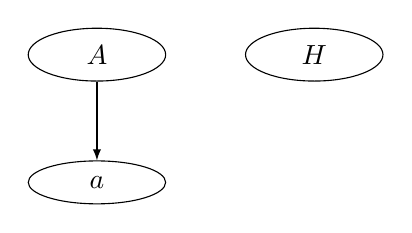
\begin{tikzpicture}[
  node distance=1cm and 1cm,
  mynode/.style={draw,ellipse,text width=1cm,align=center}
]
\node[mynode] (h1) {$A$};
\node[mynode, right =of h1] (h) {$H$};
\node[mynode, below  =of h1] (e1) {$a$};
\path 
(h1) edge[-latex] (e1);
\end{tikzpicture}

\caption{Bayesian network with wholly unrelated claim $H$.}
\label{network-unrelated}
\end{figure}
\end{center}

The intuition that the same evidence tracks the conjunction
\(A\wedge B\) better than one of the conjuncts \(A\) and \(B\) might
rest on another model of what is going on. Say \(ab\) is an item of
evidence that arises when \(A\) or \(B\) occurs with \(60\%\)
probability. That is, \(\pr{ab \vert A}=\pr{a \vert B}=60\%\). What
would be the sensitivity of \(ab\) relative to the conjunction
\(A\wedge B\), \(\pr{ab \vert A\wedge B}\)? We can represent this set up
in Figure \ref{network-ab}. Intuitvely, one might reason as follows.
There are two paths leading to \(ab\), one path starts with \(A\) and
another path starts with \(B\). When both these pathst are active, since
we are assuming \(A\wedge B\), then the probability of \(ab\) must be
higher than if just one of the two paths is active. Hence,
\(\pr{ab \vert A\wedge B}\geq 60\%\).
\todo{M: Is this true probabilistically? If not, what assumptions are required? HELP!}

\begin{center}
\begin{figure}[h!]
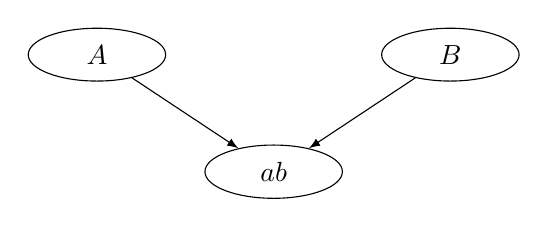
\begin{tikzpicture}[
  node distance=1cm and 1cm,
  mynode/.style={draw,ellipse,text width=1cm,align=center}
]
\node[mynode] (h1) {$A$};
\node[mynode, below right=of h1] (e) {$ab$};
\node[mynode, above right=of e] (h2) {$B$};
\path 
(h1) edge[-latex] (e)
(h2) edge[-latex] (e);
\end{tikzpicture}

\caption{Bayesian network with $ab$ resulting from $A$ and $B$.}
\label{network-ab}
\end{figure}
\end{center}

\hypertarget{but-sensitivity-depends-on-prior-probabilities}{%
\subsection{But Sensitivity Depends On Prior
Probabilities}\label{but-sensitivity-depends-on-prior-probabilities}}

We have shown, given a suitable number of assumptions, that the
sensitivity of \(a\wedge b\) can be greater relative to \(A \wedge B\)
than \(A\) alone. This explains why the evidential support of
\(a\wedge b\) is greater in favor of \(A \wedge B\) than alone \(A\).
Therefore---one might conclude---even factoring out differences in
priors probabiliies could still lead to differences in evidential
strength simply due to difference in sensitivity. But note that this
argument assumes that sensitivity---or specificity---have nothing to do
with prior probabilities.

Things are somewhat more complicated. After all,
\(\frac{\pr{a\wedge b \vert A}}{\pr{a\wedge b \vert A \wedge B}}=\frac{\pr{b \vert A}}{\pr{b \vert B}}\).
The denominator, which tracks the sensitivity of \(a\wedge b\) relative
to \(A\wedge B\) does not depend on the priors of \(A\wedge B\), but
solely on the sensitivty of \(a\) and \(b\) relative to \(A\) and \(B\).
However, the numerator, which tracks the sensitivity of \(a\wedge b\)
relative to \(a\), does depend on the priors of \(A\) (or whatvere other
hypothesis one choses to computer \(\pr{b \vert A}\) or \(\pr{b}\)).
This means that the denominator can vary depeding on the prior
probability of a chosen hypothesis. Thus, the lower the prior of \(A\),
the lower the probability of \(b\). One could still insist that here we
are not comparing the prior of a hypothesis, say \(B\), and the prior of
another hypothesis, say \(A \wedge B\). Whatever the difference in
sensitivity, it cannot be due to the difference in prior probabilities
of the hypotheses.\\
On other hand hand,
\(\frac{\pr{a\wedge b \vert A}}{\pr{a\wedge b \vert A \wedge B}}\) is
comparing two quantitities, one dependent on the priors and the other
not dependent on the priors.

More generally, the intuition that characteristics of the evidence such
as sensitivity and specificity should be indepedent of the probability
of the hypothesis of iterest turns out to be incorrect empirically. One
study in the medical literature has shown, surprisingly, that the
sensitivity of a diagnostic test is independent of the prior of the
hypothesis beign tested---say whether the patient has a medical
condition. However, specificity is dependent on the prior of the
hypothesis:

\begin{quote}
Overall, specificity tended to be
lower with higher disease prevalence; there
was no such systematic effect for sensitivity (page E537).
Source: Variation of a test’s sensitivity and specificity with disease prevalence Mariska M.G. Leeflang, Anne W.S. Rutjes, Johannes B. Reitsma, Lotty Hooft and Patrick M.M. Bossuyt
CMAJ August 06, 2013 185 (11) E537-E544; DOI: https://doi.org/10.1503/cmaj.121286
\end{quote}

\noindent The authors of the study, however, caution that

\begin{quote}
 Because sensitivity is estimated in
people with the disease of interest and specificity
in people without the disease of interest, changing the relative number of people 
with and without the disease of interest should not introduce
systematic differences. Therefore, the effects that
we found may be generated by other mechanisms that affect 
both prevalence and accuracy.
\end{quote}

So, according to the authors, changes in prevalence need not directly
affect specificity since variations in prevalence and variation in
specificity may have a common cause. Our earlier calculations about
combined specificity and sensitivity agree with experimental results,
namely, only specificity depends on the priors. Our calculations, in
fact, show that different priors for the individual claim do affect
specificity. The variation of specificity in the result of of splitting
the negation of the composite hypthesis \(\neg (A \wedge B)\) into three
further scenarios, \(\neg A \wedge B\), \(B \wedge \neg A\) and
\(\neg A \wedge neg B\). This prior sensitivity, of course, only applies
to composite hyotheses, but to some extent, any hypothesis can be
analyzed as a composite hypothesis. The claim that the defedant was
running down 5th avnue can be broken down in the conjuction that the
defendant was running and that the defendant was at 5th avenue. Any
claim, under some level of description, is a composite hypothesis. So,
perhpas, the quality or strength of the evidence should depend on the
the priors whether the hypothesis is composite or not. Is this another
example of base rate neglect?
\todo{M: Might be good to have a simulation here that makes vidid why combined specificity is in fact dependent on the priors. Maybe it is, after all, a fallacy 
to think that the quality/strength of the evidence should be independent of the priors. HELP!}

Let's grant that the quality of the evidence should depend, contrary to
our initial intuition, on the prior probability of the hypotheses. If
that is so, it would not be natural to see that evidence -- the same
evidence -- strongly favors \(A\wedge B\) without strongly favoring
\(A\) or \(B\). Perhaps we can make sense of this if we keep in mind the
comparison between hypothesis we are making here.

NOT SURE HOW TO CONTINUE HERE THOUGH!

TO DO:

\begin{enumerate}
\def\labelenumi{\arabic{enumi}.}
\item
  NOTE THAT EVEN BY EQUALIZING PRIORS, TE DISTRBUTION PARADOX DOES NOT
  GO AWAY. SO WHAT ELSE IS GOING ON HERE? NEED TO MAKE COMPATISON
  BETWEEN HYPOTHESES. NEED TO FIGURE THIS OUT!
\item
  TRY TO MAKE SENSE OF THIS, IT IS INTITVELY ACCEPTABLE THAT SUPPORT FOR
  COMBINED CLAIM, EVEN HOLDING FIXED THE SAME EVIDENCE, SHOULD BE
  STRONGER THEN SUPPORT FOR INDIVIDUAL CLAIM? THAT IS CLEARLY ODD AND
  GOES AGAINST COMMON ASSUMPTIONS.
\item
  \textbf{HYPOTHESIS: WHEN THE HYPTHESIS IS NOT MEDIATED (AS IN a toward A OR b TOWARD B, AS OPPOSED TO a TOWARD A-AND-B), THEN SENSITIVITY OR SPECICITIY IS NOT DEPEDENT ON PRIORS}
\end{enumerate}

\hypertarget{which-measure-of-combined-evidential-support}{%
\subsection{Which Measure of (Combined) Evidential
Support?}\label{which-measure-of-combined-evidential-support}}

THIGNS TO ADD:

\begin{enumerate}
\def\labelenumi{\arabic{enumi}.}
\item
  THE MIN SEEMS TO BE THE MEASURE FOR COMPOSITE CLAIMS THAT CAPTURES
  AGGREGATION AND DISTRIBUTION BEST. SO THE QUESTION IS WHAT
  PROBABILISTIC MEASURE CAPTURES MIN?
\item
  IS DEPEDENCY ON PRIOR ANOTHER EXAMPLE OF BASE RATE NEGLECT? WE NEGLECT
  BAE RATE IN CALCULATING POSTERIOR BUT ALSO IN CALCULATING STRENGTH OF
  EVIDENCE? WE JUST NEED TO LIVE WITH THE FACT THAT WE HAVE A POOR
  UNDERSTANDING OF EVIDENCE BUT PERHPAS GOOD ENOUGH TO GET BY IN THE
  WORLD. CONNECT TO POINT 1 AND MIN FUNCTION.
\end{enumerate}

\hypertarget{the-likelihood-strategy}{%
\subsection{The likelihood strategy}\label{the-likelihood-strategy}}

Focusing on posterior probabilities is not the only approach that legal
probabilists can pursue. By Bayes' theorem, the following holds, using
\(G\) and \(I\) as competing hypotheses:

\[ \frac{\Pr(G \vert E)}{\Pr(I \vert E)} = \frac{\Pr(E \vert G)}{\Pr(E \vert I)} \times \frac{\Pr(G)}{\Pr(I)},\]

or using \(H_p\) and \(H_d\) as competing hypotheses,

\[ \frac{\Pr(H_p \vert E)}{\Pr(H_d \vert E)} = \frac{\Pr(E \vert H_p)}{\Pr(E \vert H_d)} \times \frac{\Pr(H_p)}{\Pr(H_d)},\]

or in words

\[ \textit{posterior odds} = \textit{likelihood ratio} \times \textit{prior odds}.\]

A difficult problem is to assign numbers to the prior probabiliteis such
as \(\Pr(G)\) or \(\Pr(H_p)\), or priors odds such as
\(\frac{\Pr(G)}{\Pr(I)}\) or \(\frac{\Pr(H_p)}{\Pr(H_d)}\).

DISCUSS DIFFICULTIES ABOUT ASSIGNING PRIORS! WHERE? CAN WE USE IMPRECISE
PROBABILKITIES T TALK ABOUT PRIORS -- I.E. LOW PRIORS = TOTAL IGNORANCE
= VERY IMPRECISE (LARGE INTERVAL) PRIORS? THE PROBLME WITH THIS WOULD BE
THAT THERE IS NO UPDSATING POSSIBLE. ALL UPDATING WOULD STILL GET BACK
TO THE STARTING POINT. DO YOU HAVE AN ANSWER TO THAT? WOULD BE
INTERETSING TO DISCUSS THIS!

Given these difficulties, both practical and theoretical, one option is
to dispense with priors altogether. This is not implausible. Legal
disputes in both criminal and civil trials should be decided on the
basis of the evidence presented by the litigants. But it is the
likelihood ratio -- not the prior ratio -- that offers the best measure
of the overall strength of the evidece presented. So it is all too
natural to focus on likekihood ratios and leave the priors out of the
picture. If this is the right, the question is, how would a
probabilistic interpretation of standards of proof based on the
likelihood rato look like? At its simplest, this stratgey will look as
follows. Recall our discussion of expected utility theory:

\[ \text{convict provided}           \frac{cost(CI)}{cost(AG)} < \frac{\Pr(H_p \vert E)}{\Pr(H_d \vert E )}, \]

which is equivalent to

\[ \text{convict provided}           \frac{cost(CI)}{cost(AG)} < \frac{\Pr(E \vert H_p)}{\Pr(E \vert H_d)} \times \frac{\Pr(H_p)}{\Pr(H_d)}.\]

By rearraing the terms,

\[ \text{convict provided}  \frac{\Pr(E \vert H_p)}{\Pr(E \vert H_d)} > \frac{\Pr(H_d)}{\Pr(H_p)} \times     \frac{cost(CI)}{cost(AG)} .\]

Then, on this intepretation, the likelihood ratio should be above a
suitable threshold that is a function of the cost ratio and the prior
ratio. The outstanding question is how this threshold is to be
determined.

\hypertarget{kaplow}{%
\subsubsection{Kaplow}\label{kaplow}}

Quite independently, a similar approach to juridical decisions has been
proposed by Kaplow (2014) -- we'll call it
\textbf{decision-theoretic legal probabilism (DTLP)}. It turns out that
Cheng's suggestion is a particular case of this more general approach.
Let \(LR(E)=\pr{E\vert H_\Pi}/\pr{E\vert H_\Delta}\). In whole
generality, DTLP invites us to convict just in case \(LR(E)>LR^\star\),
where \(LR^\star\) is some critical value of the likelihood ratio.

Say we want to formulate the usual preponderance rule: convict iff
\(\pr{H_\Pi\vert E}>0.5\), that is, iff
\(\frac{\pr{H_\Pi\vert E}}{\pr{H_\Delta\vert E}}>1\). By Bayes' Theorem
we have:

\vspace{-6mm}

\begin{align*}
\frac{\pr{H_\Pi\vert E}}{\pr{H_\Delta\vert E}} =  \frac{\pr{H_\Pi}}{\pr{H_\Delta}}\times \frac{\pr{E\vert H_\Pi}}{\pr{E\vert H_\Delta}} &>1 \Leftrightarrow\\
  \Leftrightarrow \frac{\pr{E\vert H_\Pi}}{\pr{E\vert H_\Delta}} &> \frac{\pr{H_\Delta}}{\pr{H_\Pi}} 
 \end{align*} \noindent So, as expected, \(LR^\star\) is not unique and
depends on priors. Analogous reformulations are available for thresholds
other than \(0.5\).

Kaplow's point is not that we can reformulate threshold decision rules
in terms of priors-sensitive likelihood ratio thresholds. Rather, he
insists, when we make a decision, we should factor in its consequences.
Let \(G\) represent potential gain from correct conviction, and \(L\)
stand for the potential loss resulting from mistaken conviction. Taking
them into account, Kaplow suggests, we should convict if and only if:

\vspace{-6mm}

\begin{align}
\label{eq:Kaplow_decision}
\pr{H_\Pi\vert E}\times G > \pr{H_\Delta\vert E}\times L
\end{align} \noindent Now, \eqref{eq:Kaplow_decision} is equivalent to:

\vspace{-6mm}

\begin{align}
\nonumber
\frac{\pr{H_\Pi \vert E}}{\pr{H_\Delta \vert E}} & > \frac{L}{G}\\
\nonumber
\frac{\pr{H_\Pi}}{\pr{H_\Delta}} \times \frac{\pr{E\vert H_\Pi}}{\pr{E\vert H_\Delta}} &> \frac{L}{G}\\
\nonumber
\frac{\pr{E\vert H_\Pi}}{\pr{E\vert H_\Delta}}  & > \frac{\pr{H_\Delta}}{\pr{H_\Pi}} \times \frac{L}{G}\\
\label{eq:Kaplow_decision2} LR(E)  & > \frac{\pr{H_\Delta}}{\pr{H_\Pi}} \times \frac{L}{G}
\end{align}

\noindent This is the general format of Kaplow's decision standard.

\hypertarget{dawid}{%
\subsubsection{Dawid}\label{dawid}}

Here is a slightly different perspective, due to Dawid (1987), that also
suggests that juridical decisions should be likelihood-based. The focus
is on witnesses for the sake of simplicity. Imagine the plaintiff
produces two independent witnesses: \(W_A\) attesting to \(A\), and
\(W_B\) attesting to \(B\). Say the witnesses are regarded as \(70\%\)
reliable and \(A\) and \(B\) are probabilistically independent, so we
infer \(\pr{A}=\pr{B}=0.7\) and \(\pr{A\et B}=0.7^2=0.49\).

But, Dawid argues, this is misleading, because to reach this result we
misrepresented the reliability of the witnesses: \(70\%\) reliability of
a witness, he continues, does not mean that if the witness testifies
that \(A\), we should believe that \(\pr{A}=0.7\). To see his point,
consider two potential testimonies:

\begin{center}
\begin{tabular}
{@{}ll@{}}
\toprule
  $A_1$ & The sun rose today. \\
   $A_2$ & The sun moved backwards through the sky today.\\
\bottomrule
\end{tabular}
\end{center}

\noindent     Intuitively, after hearing them, we would still take
\(\pr{A_1}\) to be close to 1 and \(\pr{A_2}\) to be close to 0, because
we already have fairly strong convictions about the issues at hand. In
general, how we should revise our beliefs in light of a testimony
depends not only on the reliability of the witness, but also on our
prior
convictions.\footnote{An issue that Dawid does not bring up is the interplay between our priors and our assessment of the reliability of the witnesses. Clearly, our posterior assessment of the credibility of the witness who testified $A_2$ will be lower than that of the other witness.}
And this is as it should be: as indicated by Bayes' Theorem, one and the
same testimony with different priors might lead to different posterior
probabilities.

So far so good. But how should we represent evidence (or testimony)
strength then? Well, one pretty standard way to go is to focus on how
much it contributes to the change in our beliefs in a way independent of
any particular choice of prior beliefs. Let \(a\) be the event that the
witness testified that \(A\). It is useful to think about the problem in
terms of \emph{odds, conditional odds (O)} and
\emph{likelihood ratios (LR)}:
\begin{align*} O(A)  & = \frac{\pr{A}}{\pr{\n A}}\\
 O(A\vert a) &= \frac{\pr{A\vert a}}{\pr{\n A \vert a}}  \\
 LR(a\vert A) &= \frac{\pr{a\vert A}}{\pr{a\vert \n A}}. 
\end{align*}

Suppose our prior beliefs and background knowledge, before hearing a
testimony, are captured by the prior probability measure
\(\prr{\cdot}\), and the only thing that we learn is \(a\). We're
interested in what our \emph{posterior} probability measure,
\(\prp{\cdot}\), and posterior odds should then be. If we're to proceed
with Bayesian updating, we should have:

\vspace{-6mm}

\begin{align*}
 \frac{\prp{A}}{\prp{\n A}} & = \frac{\prr{A\vert a}}{\prr{\n A\vert a}}
 =
 \frac{\prr{a\vert A}}{\prr{a\vert \n A}}
 \times
 \frac{\prr{A}}{\prr{\n A}}
  \end{align*} that is,

\vspace{-6mm}

\begin{align}
 \label{bayesodss2}
 O_{posterior}(A)& = O_{prior}(A\vert a) = \!\!\!\!\!  \!\!\!\!\!  \!\! \!\!  \underbrace{LR_{prior}(a\vert A)}_{\mbox{\footnotesize conditional likelihood ratio}}  \!\!\!\!\!   \!\!\!\!\!  \!\! \!\!   \times  O_{prior}(A)
 \end{align}

The conditional likelihood ratio seems to be a much more direct measure
of the value of \(a\), independent of our priors regarding \(A\) itself.
In general, the posterior probability of an event will equal to the
witness's reliability in the sense introduced above only if the prior is
\(1/2\).\footnote{Dawid gives no general argument, but it is not too hard to  give one. Let $rel(a)=\pr{a\vert A}=\pr{\n a\vert \n A}$. We have in the background $\pr{a\vert \n A}=1-\pr{\n a\vert \n A}=1-rel(a)$.
 We want to find the condition under which $\pr{A\vert a} = \pr{a\vert A}$. Set $\pr{A}=p$ and  start with Bayes' Theorem and the law of total probability, and go from there:
 \begin{align*}
 \pr{A\vert a}& = \pr{a\vert A}\\
 \frac{\pr{a\vert A}p}{\pr{a\vert A}p+\pr{a\vert \n A}(1-p)} &= \pr{a\vert A} \\
 \pr{a\vert A}p & = \pr{a\vert A}[\pr{a\vert A}p+\pr{a\vert \n A}(1-p)]\\
 p & = \pr{a\vert A}p + \pr{a\vert \n A} - \pr{a\vert \n A}p\\
 p &= rel(a) p + 1-rel(a)- (1-rel(a))p\\
 p & = rel(a)p +1 - rel(a) -p +rel(a)p \\
 2p & =  2rel(a)p + 1 - rel(a)  \\
 2p - 2 rel(a)p & = 1-rel(a)\\
 2p(1-rel(a)) &= 1-rel(a)\\
 2p & = 1
 \end{align*}

\noindent  First we multiplied both sides by the denominator. Then we divided both sides by $\pr{a\vert A}$ and multiplied on the right side. Then we used our background notation and information. Next, we manipulated the right-hand side algebraically and  moved  $-p$ to the left-hand side. Move $2rel(a)p$ to the left and manipulate the result algebraically to get to the last line.}

\hypertarget{likelihood-and-dac}{%
\subsection{Likelihood and DAC}\label{likelihood-and-dac}}

But how does our preference for the likelihood ratio as a measure of
evidence strength relate to DAC? Let's go through Dawid's reasoning.

A sensible way to probabilistically interpret the \(70\%\) reliability
of a witness who testifies that \(A\) is to take it to consist in the
fact that the probability of a positive testimony if \(A\) is the case,
just as the probability of a negative testimony (that is, testimony that
\(A\) is false) if \(A\) isn't the case, is
0.7:\footnote{In general setting, these are called the \emph{sensitivity} and \emph{specificity} of a test (respectively), and they don't have to be equal. For instance, a degenerate test for an illness which always responds positively, diagnoses everyone as ill, and so has sensitivity 1, but specificity 0.}
\[\prr{a\vert A}=\prr{\n a\vert\n  A}=0.7.\]
\noindent   \(\prr{a\vert \n A}=1- \prr{\n a\vert \n A}=0.3\), and so
the same information is encoded in the appropriate likelihood ratio:
\[LR_{prior}(a\vert A )=\frac{\prr{a\vert A}}{\prr{a\vert \n A}}= \frac{0.7}{0.3}\]

Let's say that \(a\) \emph{provides (positive) support} for \(A\) in
case \[O_{posterior}(A)=O_{prior}(A\vert a)> O_{prior}(A)\]
\noindent  that is, a testimony \(a\) supports \(A\) just in case the
posterior odds of \(A\) given \(a\) are greater than the prior odds of
\(A\) (this happens just in case \(\prp{A}>\prr{A}\)). By
\eqref{bayesodss2}, this will be the case if and only if
\(LR_{prior}(a\vert A)>1\).

One question that Dawid addresses is this: assuming reliability of
witnesses \(0.7\), and assuming that \(a\) and \(b\), taken separately,
provide positive support for their respective claims, does it follow
that \(a \et b\) provides positive support for \(A\et B\)?

Assuming the independence of the witnesses, this will hold in
non-degenerate cases that do not involve extreme probabilities, on the
assumption of independence of \(a\) and \(b\) conditional on all
combinations: \(A\et B\), \(A\et \n B\), \(\n A \et B\) and
\(\n A \et \n B\).\footnote{Dawid only talks about the independence of witnesses without reference to  conditional independence. Conditional independence does not follow from independence, and it is the former that is needed here (also, four non-equivalent different versions of it).}\(^,\)\textasciitilde{}\footnote{In terms of notation and derivation in the optional content that will follow, the claim holds  if and only if $28 > 28 p_{11}-12p_{00}$.  This inequality is not  true for all admissible values of $p_{11}$ and $p_{00}$. If $p_{11}=1$ and $p_{00}=0$, the sides are equal. However, this is a rather degenerate example. Normally, we are  interested in cases where $p_{11}< 1$. And indeed, on this assumption, the inequality holds.}

Let us see why the above claim holds. The calculations are my
reconstruction and are not due to Dawid. The reader might be annoyed
with me working out the mundane details of Dawid's claims, but it turns
out that in the case of Dawid's strategy, the devil is in the details.
The independence of witnesses gives us: \begin{align*}
 \pr{a \et b \vert A\et B}& =0.7^2=0.49\\
 \pr{a \et b \vert A\et \n B}& =  0.7\times 0.3=0.21\\
 \pr{a \et b \vert \n A\et B}& =  0.3\times 0.7=0.21\\
 \pr{a \et b \vert \n A\et \n B}& =  0.3\times 0.3=0.09
 \end{align*} Without assuming \(A\) and \(B\) to be independent, let
the probabilities of \(A\et B\), \(\n A\et B\), \(A\et \n B\),
\(\n A\et \n B\) be \(p_{11}, p_{01}, p_{10}, p_{00}\). First, let's see
what \(\pr{a\et b}\) boils down to.

By the law of total probability we have:
\begin{align}\label{eq:total_lower}
 \pr{a\et b} & = 
                     \pr{a\et b \vert A \et B}\pr{A\et B} + \\ &  \nonumber
                     +\pr{a\et b \vert A \et \n B}\pr{A\et \n B} \\ &  \nonumber
 + \pr{a\et b \vert \n A \et B}\pr{\n A\et B} + \\ & \nonumber
                     + \pr{a\et b \vert \n A \et \n B}\pr{\n A\et \n B}
 \end{align} \noindent which, when we substitute our values and
constants, results in: \begin{align*}
                     & = 0.49p_{11}+0.21(p_{10}+p_{01})+0.09p_{00}
 \end{align*} Now, note that because \(p_{ii}\)s add up to one, we have
\(p_{10}+p_{01}=1-p_{00}-p_{11}\). Let us continue. \begin{align*}
    & = 0.49p_{11}+0.21(1-p_{00}-p_{11})+0.09p_{00} \\
                     & = 0.21+0.28p_{11}-0.12p_{00}
 \end{align*}

Next, we ask what the posterior of \(A\et B\) given \(a\et b\) is (in
the last line, we also multiply the numerator and the denominator by
100). \begin{align*}
 \pr{A\et B\vert a \et b} & =
         \frac{\pr{a\et b \vert A \et B}\pr{A\et B}}
             {\pr{a\et b}}\\
         & =
                     \frac{49p_{11}}
                           {21+28p_{11}-12p_{00}} 
         \end{align*}

In this particular case, then, our question whether
\(\pr{A\et B\vert a\et b}>\pr{A\et B}\) boils down to asking whether
\[\frac{49p_{11}}{21+28p_{11}-12p_{00}}> p_{11}\] that is, whether
\(28 > 28 p_{11}-12p_{00}\) (just divide both sides by \(p_{11}\),
multiply by the denominator, and manipulate algebraically).

Dawid continues working with particular choices of values and provides
neither a general statement of the fact that the above considerations
instantiate nor a proof of it. In the middle of the paper he says:

\begin{quote}
 Even under prior dependence, the combined support is always positive, in the sense that the posterior probability of the case always exceeds its prior probability\dots When the problem is analysed carefully, the `paradox' evaporates [pp. 95-7]\end{quote}

\noindent where he still means the case with the particular values that
he has given, but he seems to suggest that the claim generalizes to a
large array of cases.

The paper does not contain a precise statement making the conditions
required explicit and, \emph{a fortriori}, does not contain a proof of
it. Given the example above and Dawid's informal reading, let us develop
a more precise statement of the claim and a proof thereof.

\begin{fact}\label{ther:increase}
Suppose that  $rel(a),rel(b)>0.5$ and witnesses are independent conditional on all Boolean combinations of $A$ and $B$  (in a sense to be specified), and that none of the Boolean combinations of $A$ and $B$ has an extreme probability (of 0 or 1). It follows that  $\pr{A\et B \vert a\et b}>\pr{A\et B}$. (Independence of $A$ and $B$ is not required.)
\end{fact}

Roughly, the theorem says that if independent and reliable witnesses
provide positive support of their separate claims, their joint testimony
provides positive support of the conjunction of their claims.

Let us see why the claim holds. First, we introduce an abbreviation for
witness reliability:
\begin{align*}\mathbf{a} &=rel(a)=\pr{a\vert A}=\pr{\n a\vert \n A}>0.5\\ 
\mathbf{b} &=rel(b)=\pr{b\vert B}=\pr{\n b\vert \n A}>0.5
\end{align*} Our independence assumption means: \begin{align*}
\pr{a\et b \vert A\et B}  &= \mathbf{ab}\\
\pr{a\et b \vert A\et \n B} & = \mathbf{a(1-b)}\\
\pr{a\et b \vert \n A\et B}  & = \mathbf{(1-a)b}\\
\pr{a\et b \vert \n A\et \n  B}  & = \mathbf{(1-a)(1-b)}
\end{align*}

\vspace{-2mm}

Abbreviate the probabilities the way we already did:

\begin{center}
\begin{tabular}{ll}
$\pr{A\et B} = p_{11}$ & $\pr{A\et \n B} = p_{10}$\\
$\pr{\n A \et B} = p_{01}$ & $\pr{\n A \et \n B}=p_{00}$
\end{tabular}
\end{center}

Our assumptions entail \(0\neq p_{ij}\neq 1\) for \(i,j\in \{0,1\}\)
and: \begin{align}\label{eq:sumupto1}
p_{11}+p_{10}+p_{01}+p_{00}&=1
\end{align}

\noindent So, we can use this with \eqref{eq:total_lower} to get:
\begin{align}\label{eq:aetb}
\pr{a\et b} & =  \mathbf{ab}p_{11} + \mathbf{a(1-b)}p_{10}+\mathbf{(1-a)b}p_{01} + \mathbf{(1-a)(1-b)}p_{00}\\ \nonumber
& = p_{11}\mathbf{ab} + p_{10}(\mathbf{a}-\mathbf{ab}) + p_{01}(\mathbf{b}-\mathbf{ab})+p_{00}(1-\mathbf{b}-\mathbf{a}+\mathbf{ab})
\end{align}

Let's now work out what the posterior of \(A\et B\) will be, starting
with an application of the Bayes' Theorem: \begin{align} \nonumber
\pr{A\et B \vert a\et b} & = \frac{\pr{a\et b \vert A \et B}\pr{A\et B}}{\pr{a\et b}}
\\ \label{eq:boiled}
& = \frac{\mathbf{ab}p_{11}}{p_{11}\mathbf{ab} + p_{10}(\mathbf{a}-\mathbf{ab}) + p_{01}(\mathbf{b}-\mathbf{ab})+p_{00}(1-\mathbf{b}-\mathbf{a}+\mathbf{ab})}
\end{align} To answer our question we therefore have to compare the
content of \eqref{eq:boiled} to \(p_{11}\) and our claim holds just in
case: \begin{align*}
\frac{\mathbf{ab}p_{11}}{p_{11}\mathbf{ab} + p_{10}(\mathbf{a}-\mathbf{ab}) + p_{01}(\mathbf{b}-\mathbf{ab})+p_{00}(1-\mathbf{b}-\mathbf{a}+\mathbf{ab})} &> p_{11}
\end{align*} \begin{align*}
 \frac{\mathbf{ab}}{p_{11}\mathbf{ab} + p_{10}(\mathbf{a}-\mathbf{ab}) + p_{01}(\mathbf{b}-\mathbf{ab})+p_{00}(1-\mathbf{b}-\mathbf{a}+\mathbf{ab})} & > 1\end{align*}
\begin{align}  
 \label{eq:goal}
p_{11}\mathbf{ab} + p_{10}(\mathbf{a}-\mathbf{ab}) + p_{01}(\mathbf{b}-\mathbf{ab})+p_{00}(1-\mathbf{b}-\mathbf{a}+\mathbf{ab}) & < \mathbf{ab}
\end{align} Proving \eqref{eq:goal} is therefore our goal for now. This
is achieved by the following
reasoning:\footnote{Thanks to Pawel Pawlowski for working on this proof with me.}

\hspace{-7mm}
\resizebox{13.5cm}{!}{
\begin{tabular}{llr}
 1. & $\mathbf{b}>0.5,\,\,\, \mathbf{a}>0.5$ & \mbox{assumption}\\
 2. & $2\mathbf{b}>1,\,\,\, 2\mathbf{a}> 1$ & \mbox{from 1.}\\
 3. & $2\mathbf{ab}>\mathbf{a},\,\,\, 2\mathbf{ab}>\mathbf{b}$ & \mbox{multiplying by $\mathbf{a}$ and $\mathbf{b}$ respectively}\\
 4.  & $p_{10}2\mathbf{ab}>p_{10}\mathbf{a}$,\,\,\, $p_{01}2\mathbf{ab}>p_{01}\mathbf{b}$ & \mbox{multiplying by $p_{10}$ and $p_{01}$ respectively}\\
 5.  & $p_{10}2\mathbf{ab} +  p_{01}2\mathbf{ab} > p_{10}\mathbf{a} + p_{01}\mathbf{b}$ & \mbox{adding by sides, 3., 4.}\\
 6. & $1- \mathbf{b}- \mathbf{a} <0$ & \mbox{from 1.}\\
 7. & $p_{00}(1-\mathbf{b}-\mathbf{a})<0$ & \mbox{From 6., because $p_{00}>0$}\\
  8.  &  $p_{10}2\mathbf{ab} +  p_{01}2\mathbf{ab} > p_{10}\mathbf{a} + p_{01}\mathbf{b} + p_{00}(1-\mathbf{b}-\mathbf{a})$ & \mbox{from 5. and 7.}\\
  9.  & $p_{10}\mathbf{ab} + p_{10}\mathbf{ab} + p_{01}\mathbf{ab} + p_{01}\mathbf{ab} + p_{00}\mathbf{ab} - p_{00}\mathbf{ab}> p_{10}\mathbf{a} + p_{01}\mathbf{b} + p_{00}(1-\mathbf{b}-\mathbf{a})$ & \mbox{8., rewriting left-hand side}\\
  10.  & $p_{10}\mathbf{ab} + p_{01}\mathbf{ab}  + p_{00}\mathbf{ab} > - p_{10}\mathbf{ab}  -  p_{01}\mathbf{ab} + p_{00}\mathbf{ab} +  p_{10}\mathbf{a} + p_{01}\mathbf{b} + p_{00}(1-\mathbf{b}-\mathbf{a})$ &  \mbox{9., moving from left to right}\\
11. & $\mathbf{ab}(p_{10}+p_{01}+p_{00})> p_{10}(\mathbf{a}-\mathbf{ab})+p_{01}(\mathbf{b}-\mathbf{ab})+p_{00}(1-\mathbf{b}-\mathbf{a}+\mathbf{ab})$ & \mbox{10., algebraic manipulation}\\
12. & $\mathbf{ab}(1-p_{11})> p_{10}(\mathbf{a}-\mathbf{ab})+p_{01}(\mathbf{b}-\mathbf{ab})+p_{00}(1-\mathbf{b}-\mathbf{a}+\mathbf{ab})$ & \mbox{11. and equation \eqref{eq:sumupto1}}\\
13. & $\mathbf{ab}- \mathbf{ab}p_{11}> p_{10}(\mathbf{a}-\mathbf{ab})+p_{01}(\mathbf{b}-\mathbf{ab})+p_{00}(1-\mathbf{b}-\mathbf{a}+\mathbf{ab})$ & \mbox{12., algebraic manipulation}\\
14. & $\mathbf{ab}> \mathbf{ab}p_{11}+ p_{10}(\mathbf{a}-\mathbf{ab})+p_{01}(\mathbf{b}-\mathbf{ab})+p_{00}(1-\mathbf{b}-\mathbf{a}+\mathbf{ab})$ & \mbox{13., moving from left to right}\\
\end{tabular}}

\%\textbackslash end\{adjustbox\}

\vspace{1mm}

The last line is what we have been after.

\intermezzob

Now that we have as a theorem an explication of what Dawid informally
suggested, let's see whether it helps the probabilist handling of DAC.

\hypertarget{kaplow-1}{%
\subsubsection{Kaplow}\label{kaplow-1}}

On RLP, at least in certain cases, the decision rule leads us to
\eqref{eq:Cheng:compar2}, which tells us to decide the case based on
whether the likelihood ratio is greater than 1.

\footnote{Again, the name of the view is by no means standard, it is  just a term I coined to refer to various types of legal probabilism in a fairly uniform manner.}
While Kaplow did not discuss DAC or the gatecrasher paradox, it is only
fair to evaluate Kaplow's proposal from the perspective of these
difficulties.

Add here stuff from Marcello's Mind paper about the prisoner
hypothetical. Then, discuss Rafal's critique of the likelihood ratio
threshold and see where we end up.

\hypertarget{dawids-likelihood-strategy-doesnt-help}{%
\subsection{Dawid's likelihood strategy doesn't
help}\label{dawids-likelihood-strategy-doesnt-help}}

Recall that DAC was a problem posed for the decision standard proposed
by TLP, and the real question is how the information resulting from Fact
\ref{ther:increase} can help to avoid that problem. Dawid does not
mention any decision standard, and so addresses quite a different
question, and so it is not clear that `\texttt{the}paradox'
evaporates'\,', as Dawid suggests.

What Dawid correctly suggests (and we establish in general as Fact
\ref{ther:increase}) is that the support of the conjunction by two
witnesses will be positive as soon as their separate support for the
conjuncts is positive. That is, that the posterior of the conjunction
will be higher that its prior. But the critic of probabilism never
denied that the conjunction of testimonies might raise the probability
of the conjunction if the testimonies taken separately support the
conjuncts taken separately. Such a critic can still insist that Fact
\ref{ther:increase} does nothing to alleviate her concern. After all, at
least \emph{prima facie} it still might be the case that:

\begin{itemize}
\item  the posterior probabilities of the conjuncts are above a given threshold,
\item   the posterior probability of the conjunction is higher than the prior probability of the conjunction,
\item   the posterior probability of the conjunction 
 is still below the threshold.
\end{itemize}

That is, Fact \ref{ther:increase} does not entail that once the
conjuncts satisfy a decision standard, so does the conjunction.

At some point, Dawid makes a general claim that is somewhat stronger
than the one already cited:

\begin{quote} When the problem is analysed carefully, the `paradox' evaporates: suitably measured, the support supplied by the conjunction of several independent testimonies exceeds that supplied by any of its constituents.

  [p. 97]\end{quote}

This is quite a different claim from the content of Fact
\ref{ther:increase}, because previously the joint probability was
claimed only to increase as compared to the prior, and here it is
claimed to increase above the level of the separate increases provided
by separate testimonies. Regarding this issue Dawid elaborates (we still
use the \(p_{ij}\)-notation that we've already introduced):

\begin{quote}
 ``More generally, let $\pr{a\vert A}/\pr{a\vert \n A}=\lambda$, $\pr{b\vert B}/\pr{b\vert \n B}=\mu$, with $\lambda, \mu >0.7$, as might arise, for example, when there are several available testimonies. If the witnesses are
  independent, then \[\pr{A\et B\vert  a\et b} = \lambda \mu p_{11}/(\lambda \mu p_{11} + \lambda p_{10} +\mu p_{01} + p_{00})\] which  increases with
 each of $\lambda$ and $\mu$, and is never less than the larger of $\lambda p_{11}/(1-p_{11}+\lambda p_{11}),
 \mu p_{11} /(1- p_{11} 1 + \mu p_{11})$, the posterior probabilities appropriate to the individual testimonies.'' [p. 95]
 \end{quote}

This claim, however, is false.

\intermezzoa

Let us see why. The quoted passage is a bit dense. It contains four
claims for which no arguments are given in the paper. The first three
are listed below as \eqref{eq:lambdamu}, the fourth is that if the
conditions in \eqref{eq:lambdamu} hold,
\(\pr{A\et B\vert a\et b}>max(\pr{A\vert a},\pr{B\vert b})\). Notice
that \(\lambda=LR(a\vert A)\) and \(\mu=LR(b\vert B)\). Suppose the
first three claims hold, that is: \begin{align}\label{eq:lambdamu}
 \pr{A\et B\vert  a\et b} &= \lambda \mu p_{11}/(\lambda \mu p_{11} + \lambda p_{10} +\mu p_{01} + p_{00})\\
 \pr{A\vert a} & = \frac{\lambda p_{11}}{1-p_{11}+\lambda p_{11}}\nonumber \\
 \pr{B\vert b} & = \frac{\mu p_{11}}{1-p_{11}+\mu p_{11}} \nonumber 
 \end{align} \noindent Is it really the case that
\(\pr{A\et B\vert a\et b}>\pr{A\vert a},\pr{B\vert b}\)? It does not
seem so. Let \(\mathbf{a}=\mathbf{b}=0.6\),
\(pr =\la p_{11},p_{10},p_{01},p_{00}\ra=\la 0.1, 0.7, 0.1, 0.1 \ra\).
Then, \(\lambda=\mu=1.5>0.7\) so the assumption is satisfied. Then we
have \(\pr{A}=p_{11}+p_{10}=0.8\), \(\pr{B}=p_{11}+p_{01}=0.2\). We can
also easily compute
\(\pr{a}=\mathbf{a}\pr{A}+(1-\mathbf{a})\pr{\n A}=0.56\) and
\(\pr{b}=\mathbf{b}\pr{B}+(1-\mathbf{b})\pr{\n B}=0.44\). Yet:

\begin{align*}
 \pr{A\vert a} & = \frac{\pr{a\vert A}\pr{A}}{\pr{a}} = \frac{0.6\times 0.8}{0.6\times 0.8 + 0.4\times 0.2}\approx 0.8571 \\
 \pr{B\vert b} & = \frac{\pr{b\vert B}\pr{B}}{\pr{b}} = \frac{0.6\times 0.2}{0.6\times 0.2 + 0.4\times 0.8}\approx 0.272 \\
 \pr{A\et B \vert a \et b} & = \frac{\pr{a\et b\vert A \et B}\pr{A\et B}}{\splitfrac{\pr{a\et b \vert A\et B}\pr{A\et B}+
   \pr{a\et b\vert A\et \n B}\pr{A\et \n B} +}{+ 
 \pr{a\et b \vert \n A \et B}\pr{\n A \et B} + \pr{a\et b \vert \n A \et \n B}\pr{\n A \et \n B}}} \\
 & = \frac{\mathbf{ab}p_{11}}{
   \mathbf{ab}p_{11} + \mathbf{a}(1-\mathbf{b})p_{10} + (1-\mathbf{a})\mathbf{b}p_{01} + (1-\mathbf{a})(1-\mathbf{b})p_{00}
 }  
    \approx 0.147
 \end{align*} The posterior probability of \(A\et B\) is not only lower
than the larger of the individual posteriors, but also lower than any of
them!

So what went wrong in Dawid's calculations in \eqref{eq:lambdamu}? Well,
the first formula is correct. However, let us take a look at what the
second one says (the problem with the third one is pretty much the
same): \begin{align*}
\pr{A\vert a } & = \frac{\frac{\pr{a\vert A}}{\pr{\n a \vert A}}\times \pr{A\et B}}{\pr{\n (A\et B)}+ \frac{\pr{a\vert A}}{\pr{\n a \vert A}} \times \pr{A\et B}}
\end{align*} Quite surprisingly, in Dawid's formula for
\(\pr{A\vert a}\), the probability of \(A\et B\) plays a role. To see
that it should not take any \(B\) that excludes \(A\) and the formula
will lead to the conclusion that \emph{always} \(\pr{A\vert a}\) is
undefined. The problem with Dawid's formula is that instead of
\(p_{11}=\pr{A\et B}\) he should have used \(\pr{A}=p_{11}+p_{10}\), in
which case the formula would rather say this: \begin{align*}
\pr{A\vert a } & = \frac{\frac{\pr{a\vert A}}{\pr{\n a \vert A}}\times \pr{A}}{\pr{\n A}+ \frac{\pr{a\vert A}}{\pr{\n a \vert A}} \times \pr{A}}\\
& = \frac{\frac{\pr{a\vert A}\pr{A}}{\pr{\n a \vert A}}}{\frac{\pr{\n a\vert A}\pr{\n A}}{\pr{\n a\vert A}}+ \frac{\pr{a\vert A}\pr{A}}{\pr{\n a \vert A}}}\\
& = \frac{\pr{a\vert A}\pr{A}}{\pr{\n a\vert A}\pr{\n A} + \pr{a\vert A}\pr{A}}
\end{align*} Now, on the assumption that witness' sensitivity is equal
to their specificity, we have \(\pr{a\vert \n A}=\pr{\n a \vert A}\) and
can substitute this in the denominator:
\begin{align*} & = \frac{\pr{a\vert A}\pr{A}}{\pr{ a\vert \n A}\pr{\n A} + \pr{a\vert A}\pr{A}}\end{align*}
and this would be a formulation of Bayes' theorem. And indeed with
\(\pr{A}=p_{11}+p_{10}\) the formula works (albeit its adequacy rests on
the identity of \(\pr{a\vert \n A}\) and \(\pr{\n a \vert A}\)), and
yields the result that we already obtained: \begin{align*}
\pr{A\vert a} &= \frac{\lambda(p_{11}+p_{10})}{1-(p_{11}+p_{10})+\lambda(p_{11}+p_{10})}\\
&= \frac{1.5\times 0.8}{1- 0.8+1.5\times 0.8} \approx 0.8571
\end{align*}

The situation cannot be much improved by taking \(\mathbf{a}\) and
\(\mathbf{b}\) to be high. For instance, if they're both 0.9 and
\(pr=\la0.1, 0.7, 0.1, 0.1 \ra\), the posterior of \(A\) is
\(\approx 0.972\), the posterior of \(B\) is \(\approx 0.692\), and yet
the joint posterior of \(A\et B\) is \(0.525\).

The situation cannot also be improved by saying that at least if the
threshold is 0.5, then as soon as \(\mathbf{a}\) and \(\mathbf{b}\) are
above 0.7 (and, \emph{a fortriori}, so are \(\lambda\) and \(\mu\)), the
individual posteriors being above 0.5 entails the joint posterior being
above 0.5 as well. For instance, for \(\mathbf{a}=0.7\) and
\(\mathbf{b}=0.9\) with \(pr= \la 0.1, 0.3, 0.5, 0.1\ra\), the
individual posteriors of \(A\) and \(B\) are \(\approx 0.608\) and
\(\approx 0.931\) respectively, while the joint posterior of \(A\et B\)
is \(\approx 0.283\).

\intermezzob

The situation cannot be improved by saying that what was meant was
rather that the joint likelihood is going to be at least as high as the
maximum of the individual likelihoods, because quite the opposite is the
case: the joint likelihood is going to be lower than any of the
individual ones.

\intermezzoa

Let us make sure this is the case. We have: \begin{align*}
 LR(a\vert A) & = \frac{\pr{a\vert A}}{\pr{a\vert \n A}}\\
 &= \frac{\pr{a\vert A}}{\pr{\n a\vert  A}} \\
& =  \frac{\mathbf{a}}{\mathbf{1-a}}.
\end{align*} where the substitution in the denominator is legitimate
only because witness' sensitivity is identical to their specificity.

With the joint likelihood, the reasoning is just a bit more tricky. We
will need to know what \(\pr{a\et b \vert \n (A\et B)}\) is. There are
three disjoint possible conditions in which the condition holds:
\(A\et \n B, \n A \et B\), and \(\n A \et \n B\). The probabilities of
\(a\et b\) in these three scenarios are respectively
\(\mathbf{a(1-b),(1-a)b,(1-a)(1-b)}\) (again, the assumption of
independence is important), and so on the assumption \(\n(A\et B)\) the
probability of \(a\et b\) is: \begin{align*}
\pr{a\et b \vert \n (A\et B)} & = 
\mathbf{a}(1-\mathbf{b})+(1-\mathbf{a})\mathbf{b}+(1-\mathbf{a})(1-\mathbf{b})\\ 
& = 
\mathbf{a}(1-\mathbf{b})+(1-\mathbf{a})(\mathbf{b} + 1-\mathbf{b})\\
& = \mathbf{a}(1-\mathbf{b})+(1-\mathbf{a})\\
& = \mathbf{a}-\mathbf{a}\mathbf{b}+1-\mathbf{a} = 1- \mathbf{a}\mathbf{b}
\end{align*} So, on the assumption of witness independence, we have:
\begin{align*}
LR(a\et b \vert A \et B) & = \frac{\pr{a\et b \vert A \et B}}{\pr{a \et b\vert \n (A \et B)}} \\
& = \frac{\mathbf{ab}}{\mathbf{1-ab}}
\end{align*}

With \(0<\mathbf{a},\mathbf{b}<1\) we have \(\mathbf{ab}<\mathbf{a}\),
\(1-\mathbf{ab}>1-\mathbf{a}\), and consequently:
\[\frac{\mathbf{ab}}{\mathbf{1-ab}} < \frac{\mathbf{a}}{\mathbf{1-a}}\]
which means that the joint likelihood is going to be lower than any of
the individual ones.

\intermezzob

Fact \ref{ther:increase} is so far the most optimistic reading of the
claim that if witnesses are independent and fairly reliable, their
testimonies are going to provide positive support for the
conjunction,\textbackslash footnote\{And this is the reading that Dawid
in passing suggests: ``the combined support is always positive, in the
sense that the posterior probability of the case always exceeds its
prior probability.'\,' (Dawid, 1987: 95) and any stronger reading of
Dawid's suggestions fails. But Fact \ref{ther:increase} is not too
exciting when it comes to answering the original DAC. The original
question focused on the adjudication model according to which the
deciding agents are to evaluate the posterior probability of the whole
case conditional on all evidence, and to convict if it is above a
certain threshold. The problem, generally, is that it might be the case
that the pieces of evidence for particular elements of the claim can
have high likelihood and posterior probabilities of particular elements
can be above the threshold while the posterior joint probability will
still fail to meet the threshold. The fact that the joint posterior will
be higher than the joint prior does not help much. For instance, if
\(\mathbf{a}=\mathbf{b}=0.7\), \(pr=\la 0.1, 0.5, 0.3, 0.1\ra\), the
posterior of \(A\) is \(\approx 0.777\), the posterior of \(B\) is
\(\approx 0.608\) and the joint posterior is \(\approx 0.216\) (yes, it
is higher than the joint prior \(=0.1\), but this does not help the
conjunction to satisfy the decision standard).

To see the extent to which Dawid's strategy is helpful here, perhaps the
following analogy might be useful.\\
Imagine it is winter, the heating does not work in my office and I am
quite cold. I pick up the phone and call maintenance. A rather cheerful
fellow picks up the phone. I tell him what my problem is, and he reacts:

\vspace{1mm}

\begin{tabular}{lp{10cm}}
 --- & Oh, don't worry. \\
 --- & What do you mean? It's cold in here! \\
 --- & No no, everything is fine, don't worry.\\
 --- & It's not fine! I'm cold here! \\
 --- & Look, sir, my notion of it being warm in your office is that the building provides some improvement to what the situation would be if it wasn't there. And you agree that you're definitely warmer than you'd be if your desk was standing outside, don't you? Your, so to speak, posterior warmth is higher than your prior warmth, right? 
 \end{tabular}
 \vspace{1mm}

Dawid's discussion is in the vein of the above conversation. In response
to a problem with the adjudication model under consideration Dawid
simply invites us to abandon thinking in terms of it and to abandon
requirements crucial for the model. Instead, he puts forward a fairly
weak notion of support (analogous to a fairly weak sense of the building
providing improvement), according to which, assuming witnesses are
fairly reliable, if separate fairly reliable witnesses provide positive
support to the conjuncts, then their joint testimony provides positive
support for the conjunction.

As far as our assessment of the original adjudication model and dealing
with DAC, this leaves us hanging. Yes, if we abandon the model, DAC does
not worry us anymore. But should we? And if we do, what should we change
it to, if we do not want to be banished from the paradise of
probabilistic methods?

Having said this, let me emphasize that Dawid's paper is important in
the development of the debate, since it shifts focus on the likelihood
ratios, which for various reasons are much better measures of evidential
support provided by particular pieces of evidence than mere posterior
probabilities.

Before we move to another attempt at a probabilistic formulation of the
decision standard, let us introduce the other hero of our story: the
gatecrasher paradox. It is against DAC and this paradox that the next
model will be judged.

\intermezzoa

In fact, Cohen replied to Dawid's paper (L. J. Cohen, 1988). His reply,
however, does not have much to do with the workings of Dawid's strategy,
and is rather unusual. Cohen's first point is that the calculations of
posteriors require odds about unique events, whose meaning is usually
given in terms of potential wagers -- and the key criticism here is that
in practice such wagers cannot be decided. This is not a convincing
criticism, because the betting-odds interpretations of subjective
probability do not require that on each occasion the bet should really
be practically decidable. It rather invites one to imagine a possible
situation in which the truth could be found out and asks: how much would
we bet on a certain claim in such a situation? In some cases, this
assumption is false, but there is nothing in principle wrong with
thinking about the consequences of false assumptions.

Second, Cohen says that Dawid's argument works only for testimonial
evidence, not for other types thereof. But this claim is simply false --
just because Dawid used testimonial evidence as an example that he
worked through it by no means follows that the approach cannot be
extended. After all, as long as we can talk about sensitivity and
specificity of a given piece of evidence, everything that Dawid said
about testimonies can be repeated \emph{mutatis mutandis}.

Third, Cohen complaints that Dawid in his example worked with rather
high priors, which according to Cohen would be too high to correspond to
the presumption of innocence. This also is not a very successful
rejoinder. Cohen picked his priors in the example for the ease of
calculations, and the reasoning can be run with lower priors. Moreover,
instead of discussing the conjunction problem, Cohen brings in quite a
different problem: how to probabilistically model the presumption of
innocence, and what priors of guilt should be appropriate? This, indeed,
is an important problem; but it does not have much to do with DAC, and
should be discussed separately.

\hypertarget{problems-with-kaplows-stuff}{%
\subsection{Problem's with Kaplow's
stuff}\label{problems-with-kaplows-stuff}}

Kaplow does not discuss the conceptual difficulties that we are
concerned with, but this will not stop us from asking whether DTLP can
handle them (and answering to the negative). Let us start with DAC.

Say we consider two claims, \(A\) and \(B\). Is it generally the case
that if they separately satisfy the decision rule, then so does
\(A\et B\)? That is, do the assumptions: \begin{align*}
 \frac{\pr{E\vert A}}{\pr{E\vert \n A}}  & > \frac{\pr{\n A}}{\pr{A}} \times \frac{L}{G}\\
 \frac{\pr{E\vert B}}{\pr{E\vert \n B}}  & > \frac{\pr{\n B}}{\pr{B}} \times \frac{L}{G}
 \end{align*} \noindent entail \begin{align*}
 \frac{\pr{E\vert A\et B}}{\pr{E\vert \n (A\et B)}}  & > \frac{\pr{\n (A\et B)}}{
 \pr{A\et B}} \times \frac{L}{G}?
 \end{align*}

Alas, the answer is negative.

\intermezzoa

This can be seen from the following example. Suppose a random digit from
0-9 is drawn; we do not know the result; we are told that the result is
\(<7\) (\(E=\)`the result is \(<7\)'), and we are to decide whether to
accept the following claims:

\begin{center}
 \begin{tabular}{@{}ll@{}}
 \toprule
 $A$ & the result is $<5$. \\
 $B$  & the result is an even number.\\
 $A\et B$ & the result is an even number $<5$. \\
 \bottomrule
 \end{tabular}
 \end{center}

Suppose that \(L=G\) (this is for simplicity only --- nothing hinges on
this, counterexamples for when this condition fails are analogous).
First, notice that \(A\) and \(B\) taken separately satisfy
\eqref{eq:Kaplow_decision2}. \(\pr{A}=\pr{\n A}=0.5\),
\(\pr{\n A}/\pr{A}=1\) \(\pr{E\vert A}=1\), \(\pr{E\vert \n A}=0.4\).
\eqref{eq:Kaplow_decision2} tells us to check: \begin{align*}
 \frac{\pr{E\vert A}}{\pr{E\vert \n A}}&> \frac{L}{G}\times \frac{\pr{\n A}}{\pr{A}}\\
 \frac{1}{0.4} & > 1
 \end{align*}

\noindent so, following DTLP, we should accept \(A\).\\
For analogous reasons, we should also accept \(B\).
\(\pr{B}=\pr{\n B}=0.5\), \(\pr{\n B}/\pr{B}=1\) \(\pr{E\vert B}=0.8\),
\(\pr{E\vert \n B}=0.6\), so we need to check that indeed:
\begin{align*}
 \frac{\pr{E\vert B}}{\pr{E\vert \n B}}&> \frac{L}{G}\times \frac{\pr{\n B}}{\pr{B}}\\
 \frac{0.8}{0.6} & > 1 
 \end{align*}

But now, \(\pr{A\et B}=0.3\), \(\pr{\n (A \et B)}=0.7\),
\(\pr{\n (A\et B)}/\pr{A\et B}=2\frac{1}{3}\),
\(\pr{E\vert A \et B}=1\), \(\pr{E\vert \n (A\et B)}=4/7\) and it is
false that: \begin{align*}
 \frac{\pr{E\vert A \et B}}{\pr{E\vert \n (A\et B)}}&> \frac{L}{G}\times \frac{\pr{\n (A \et B)}}{\pr{A \et B}}\\
 \frac{7}{4} & > \frac{7}{3} 
 \end{align*}

The example was easy, but the conjuncts are probabilistically dependent.
One might ask: are there counterexamples that involve claims which are
probabilistically
independent?\footnote{Thanks to Alicja Kowalewska for pressing me on this.}

Consider an experiment in which someone tosses a six-sided die twice.
Let the result of the first toss be \(X\) and the result of the second
one \(Y\). Your evidence is that the results of both tosses are greater
than one (\(E=: X>1 \et Y>1\)). Now, let \(A\) say that \(X<5\) and
\(B\) say that \(Y<5\).

The prior probability of \(A\) is \(2/3\) and the prior probability of
\(\n A\) is \(1/3\) and so \(\frac{\pr{\n A}}{\pr{A}}=0.5\). Further,
\(\pr{E\vert A}=0.625\), \(\pr{E\vert \n A}= 5/6\) and so
\(\frac{\pr{E\vert A}}{\pr{E\vert \n A}}=0.75\) Clearly, \(0.75>0.5\),
so \(A\) satisfies the decision standard. Since the situation with \(B\)
is symmetric, so does \(B\).

Now, \(\pr{A\et B}=(2/3)^2=4/9\) and \(\pr{\n (A\et B)}=5/9\). So
\(\frac{\pr{\n(A\et B)}}{\pr{A\et B}}=5/4\). Out of 16 outcomes for
which \(A\et B\) holds, \(E\) holds in 9, so
\(\pr{E\vert A\et B}=9/16\). Out of 20 remaining outcomes for which
\(A\et B\) fails, \(E\) holds in 16, so \(\pr{E\vert \n (A\et B)}=4/5\).
Thus, \(\frac{\pr{E\vert A\et B}}{\pr{E\vert \n (A\et B)}}=45/64 <5/4\),
so the conjunction does not satisfy the decision standard.

\intermezzob

Let us turn to the gatecrasher paradox.

Suppose \(L=G\) and recall our abbreviations: \(\pr{E}=e\),
\(\pr{H_\Pi}=\pi\). DTLP tells us to convict just in case:
\begin{align*}
 LR(E) &> \frac{1-\pi}{\pi}
 \end{align*} \noindent From \eqref{eq:Cheng_lre} we already now that
\begin{align*}
 LR(E) & = \frac{0.991-0.991\pi}{0.009\pi}
 \end{align*} \noindent so we need to see whether there are any
\(0<\pi<1\) for which\\
\begin{align*}
  \frac{0.991-0.991\pi}{0.009\pi} &> \frac{1-\pi}{\pi}
 \end{align*} \noindent Multiply both sides first by \(009\pi\) and then
by \(\pi\): \begin{align*}
 0.991\pi - 0.991\pi^2 &> 0.09\pi - 0.009\pi^2
 \end{align*} \noindent Simplify and call the resulting function \(f\):
\begin{align*}
 f(\pi) = - 0.982 \pi^2 + 0.982\pi &>0 
 \end{align*} \noindent The above condition is satisfied for any
\(0<\pi <1\) (\(f\) has two zeros: \(\pi = 0\) and \(\pi = 1\)). Here is
a plot of \(f\):

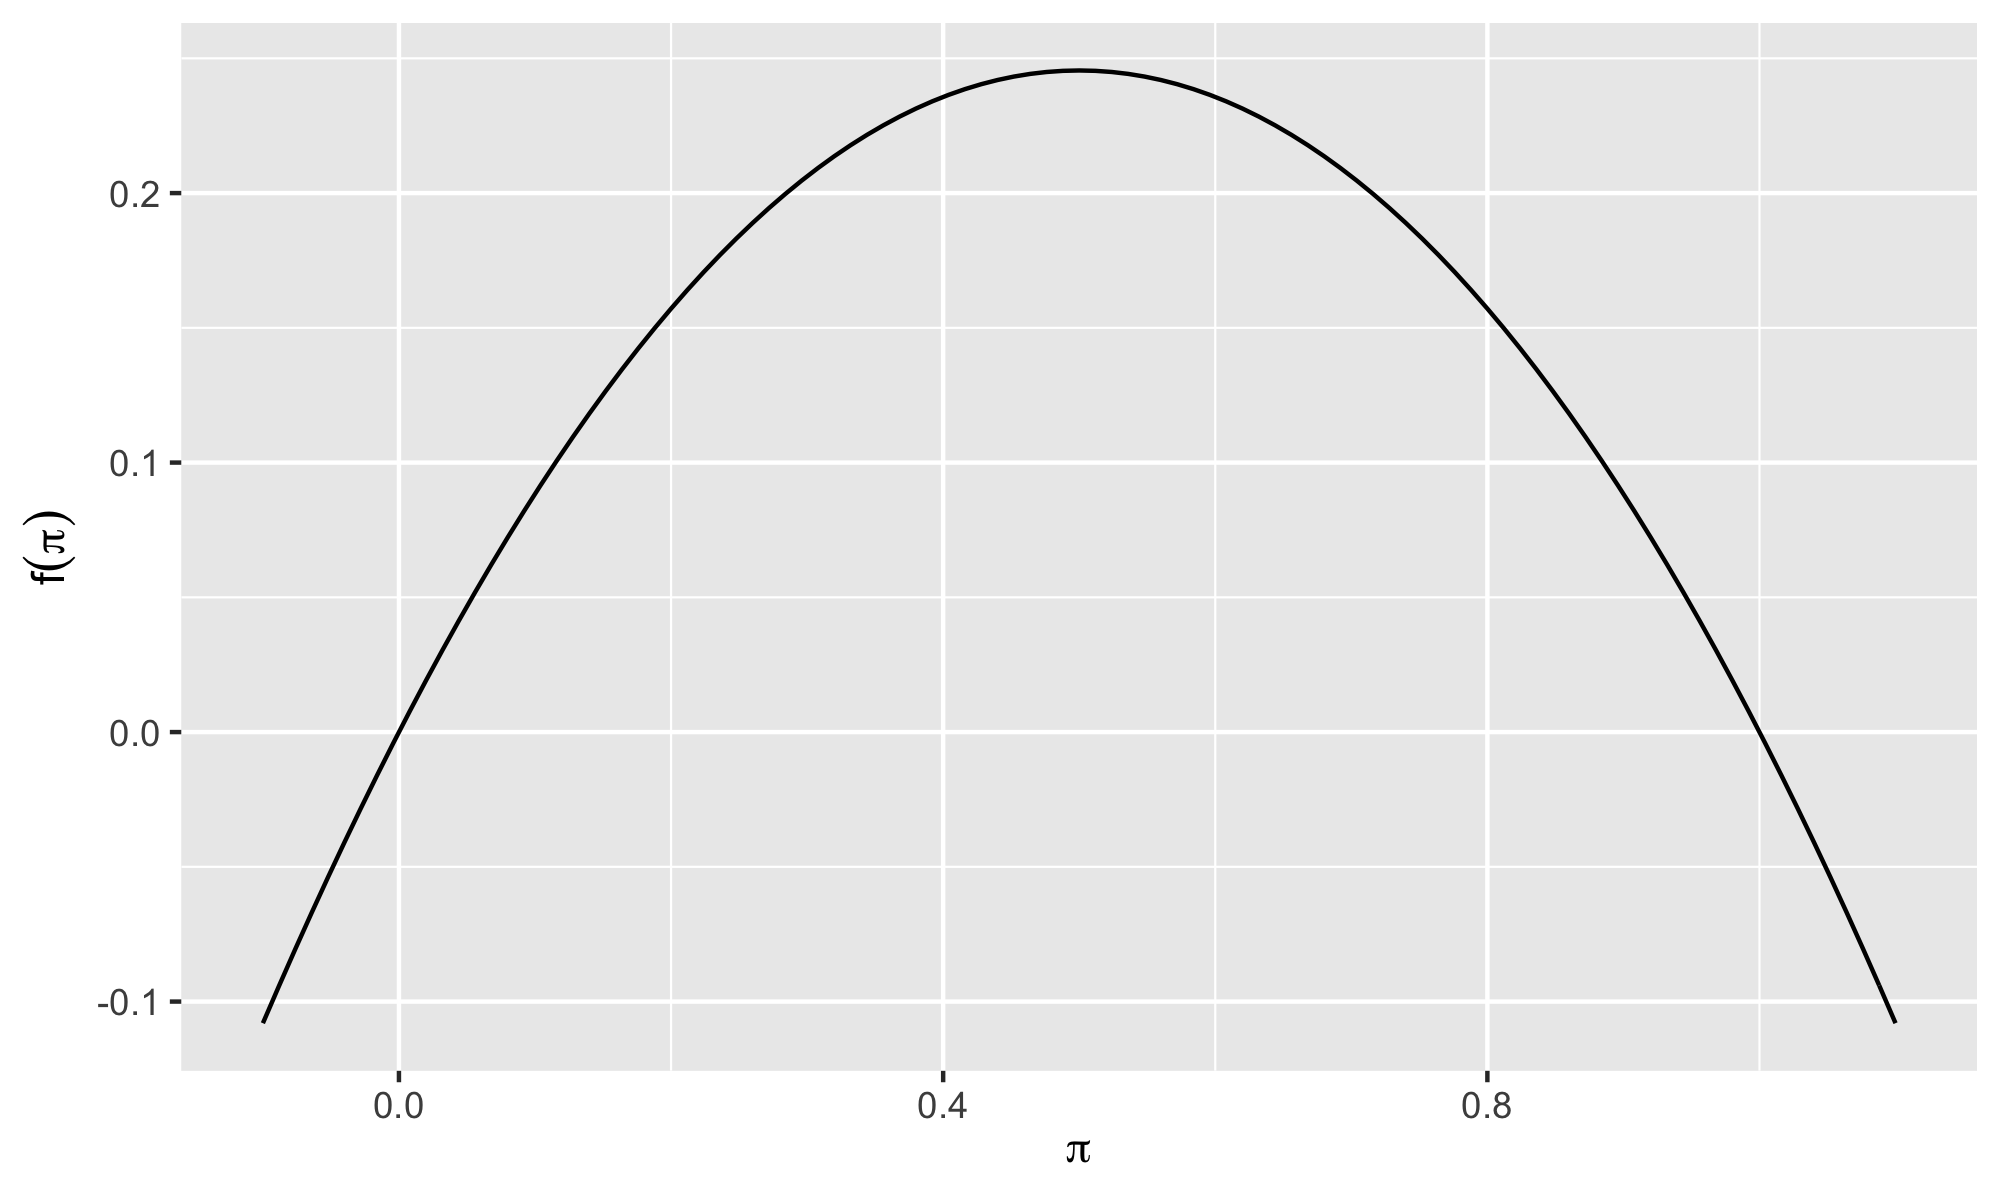
\includegraphics[width=12cm]{f-gate.png}

Similarly, \(LR(E)>1\) for any \(0< \pi <1\). Here is a plot of
\(LR(E)\) against \(\pi\):

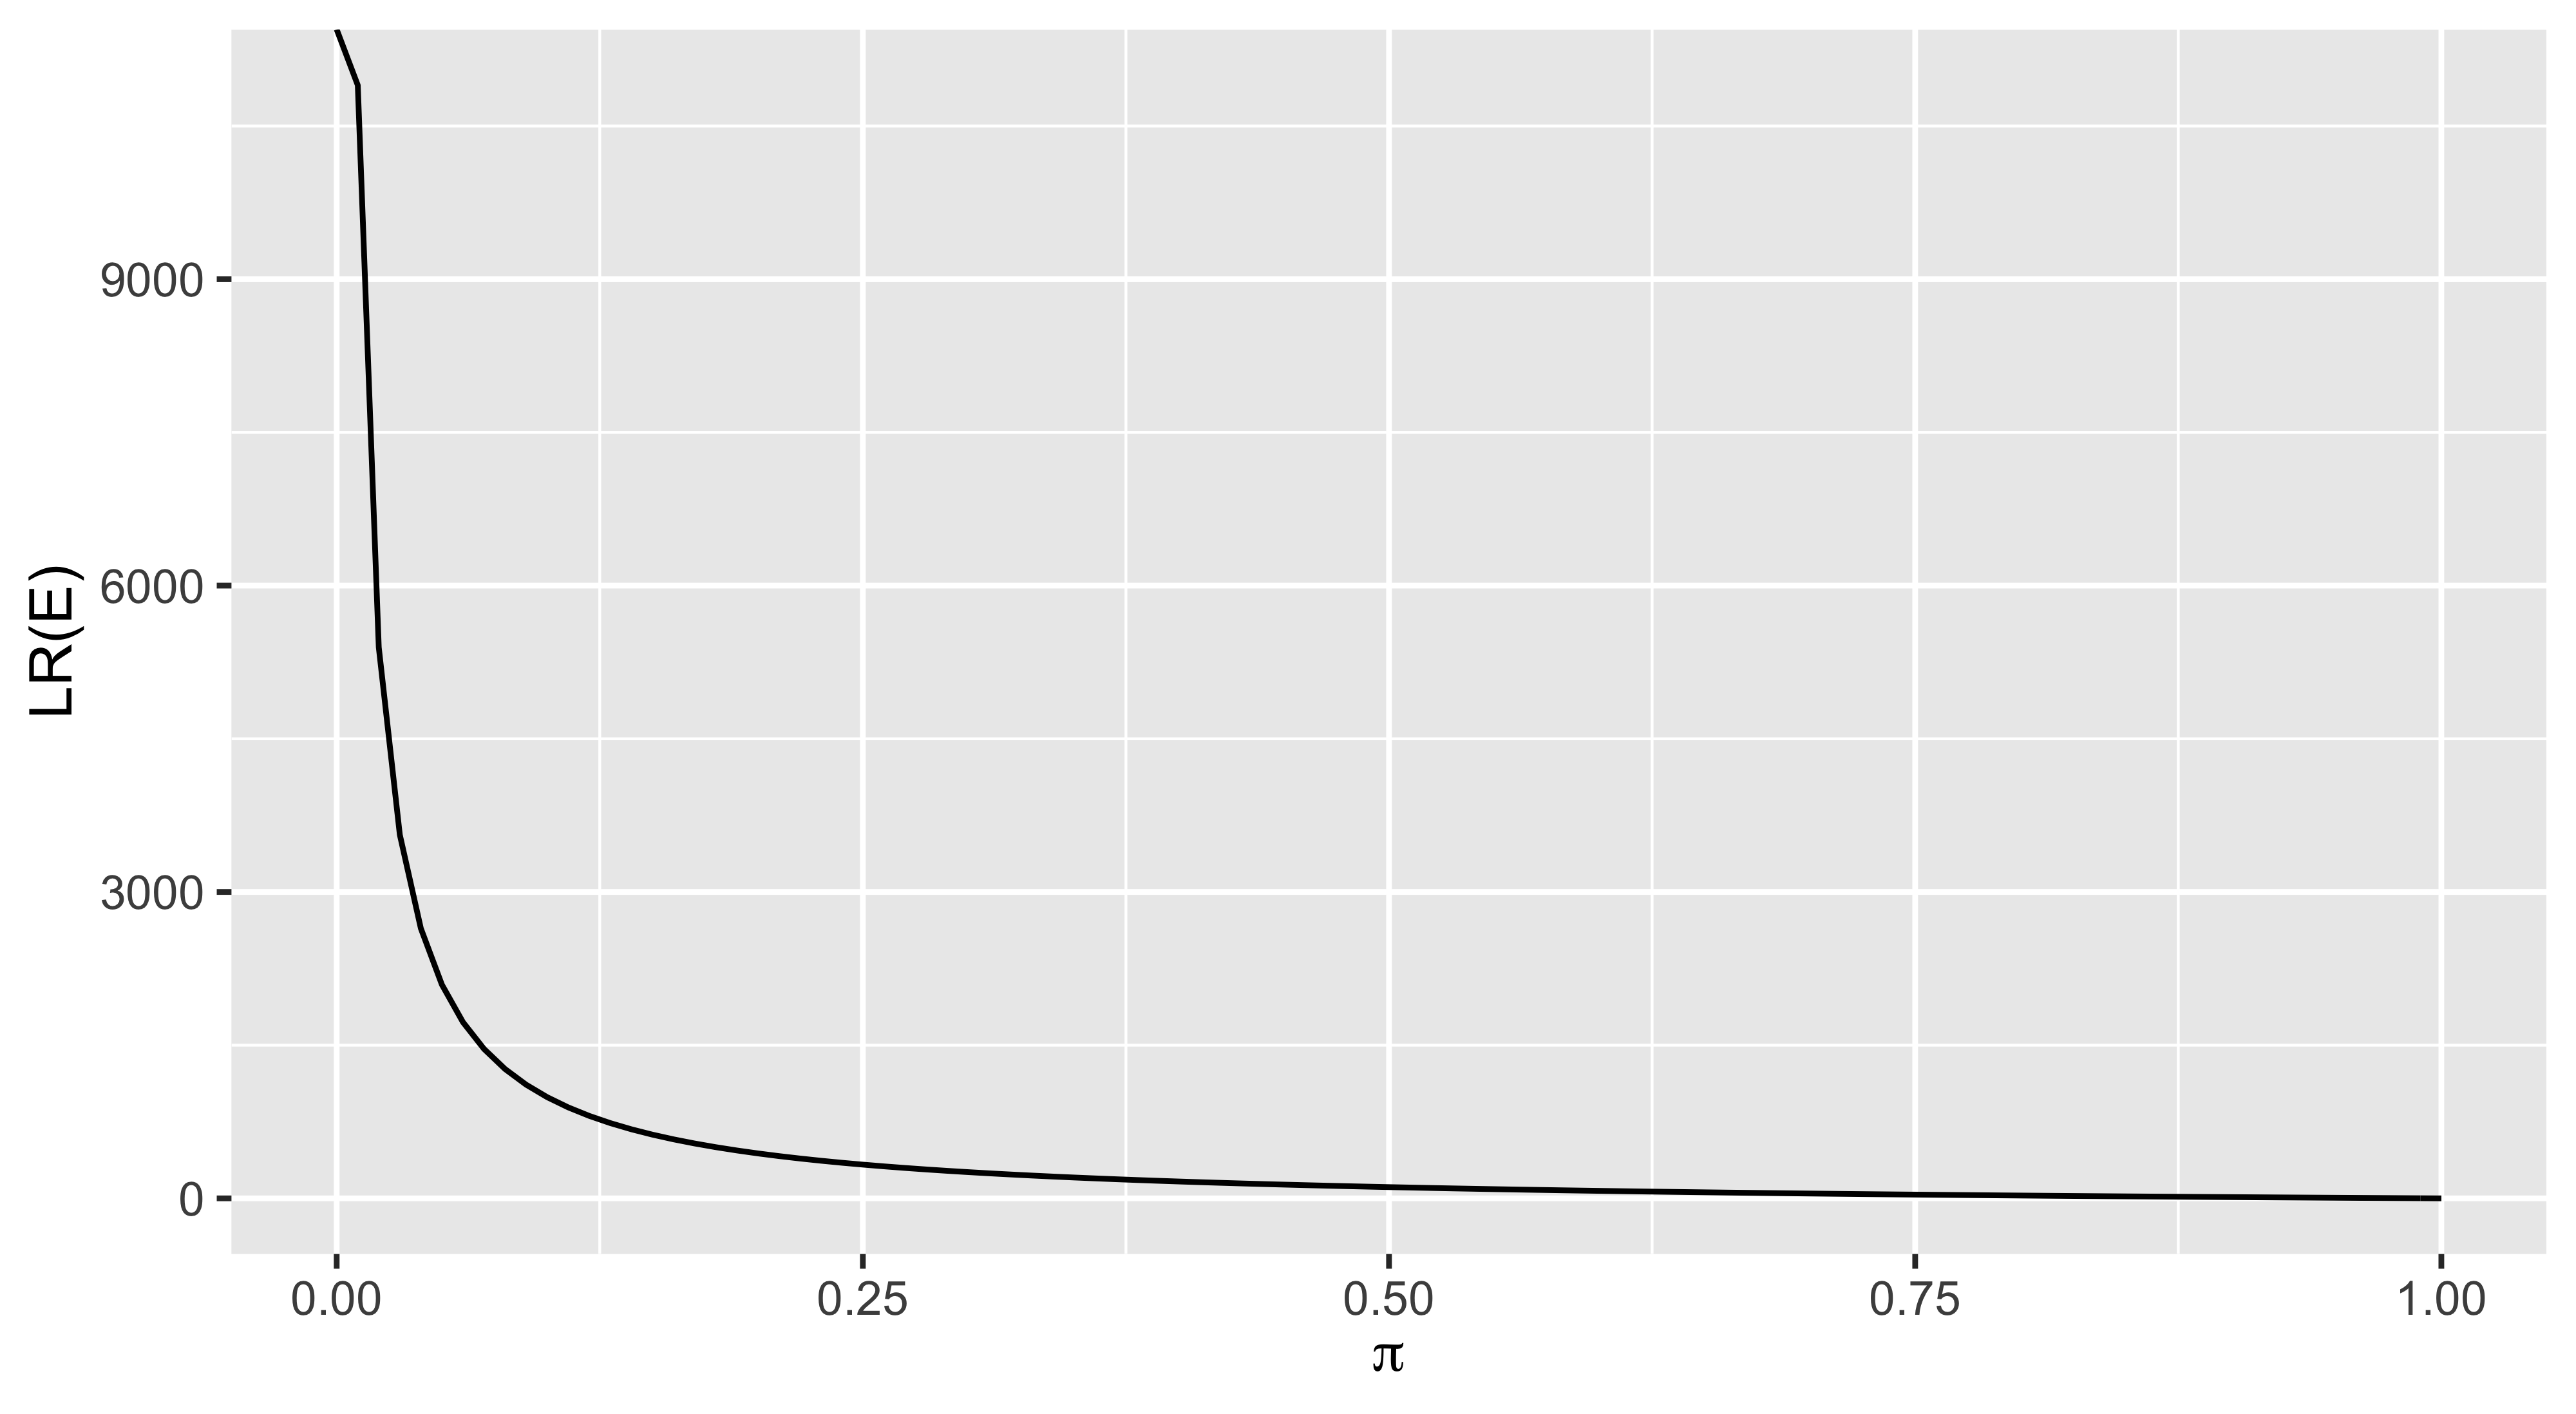
\includegraphics[width=12cm]{lre-gate.png}

\noindent Notice that \(LR(E)\) does not go below 1. This means that for
\(L=G\) in the gatecrasher scenario DTLP wold tell us to convict for any
prior probability of guilt \(\pi\neq 0,1\).

One might ask: is the conclusion very sensitive to the choice of \(L\)
and \(G\)? The answer is, not too much.

\intermezzoa

How sensitive is our analysis to the choice of \(L/G\)? Well, \(LR(E)\)
does not change at all, only the threshold moves. For instance, if
\(L/G=4\), instead of \(f\) we end up with \begin{align*}
 f'(\pi) = - 0.955 \pi^2 + 0.955\pi &>0 
 \end{align*} and the function still takes positive values on the
interval \((0,1)\). In fact, the decision won't change until \(L/G\)
increases to \(\approx 111\). Denote \(L/G\) as \(\rho\), and let us
start with the general decision standard, plugging in our calculations
for \(LR(E)\): \begin{align*}
LR(E) &> \frac{\pr{H_\Delta}}{\pr{H_\Pi}} \rho\\
LR(E) &> \frac{1-\pi}{\pi} \rho \\
\frac{0.991-0.991\pi}{0.009\pi} &> \frac{1-\pi}{\pi} \rho\\
\frac{0.991-0.991\pi}{0.009\pi}\frac{\pi}{1-\pi} &>  \rho\\
\frac{0.991\pi-0.991\pi^2}{0.009\pi-0.009\pi^2} &>  \rho\\
\frac{\pi(0.991-0.991\pi)}{\pi(0.009-0.009\pi)} &>  \rho\\
\frac{0.991-0.991\pi}{0.009-0.009\pi} &>  \rho\\
\frac{0.991(1-\pi)}{0.009(1-\pi)} &>  \rho\\
\frac{0.991}{0.009} &>  \rho\\
110.1111 &>  \rho\\
\end{align*}

\intermezzob

So, we conclude, in usual circumstances, DTLP does not handle the
gatecrasher paradox.

\hypertarget{conclusions}{%
\subsection{Conclusions}\label{conclusions}}

Where are we, how did we get here, and where can we go from here? We
were looking for a probabilistically explicated condition \(\Psi\) such
that the trier of fact, at least ideally, should accept any relevant
claim (including \(G\)) just in case \(\Psi(A,E)\).

From the discussion that transpired it should be clear that we were
looking for a \(\Psi\) satisfying the following desiderata:

\begin{description}
\item[conjunction closure] If $\Psi(A,E)$ and $\Psi(B,E)$, then $\Psi(A\et B,E)$.
\item[naked statistics] The account should at least make it possible for convictions based on strong, but naked statistical evidence to be unjustified. 
\item[equal treatment] the condition should apply to any relevant claim whatsoever (and not just a selected claim, such as $G$).
\end{description}

Throughout the paper we focused on the first two conditions (formulated
in terms of the difficulty with conjunction (DAC), and the gatecrasher
paradox), going over various proposals of what \(\Psi\) should be like
and evaluating how they fare. The results can be summed up in the
following table:

\begin{center}
\footnotesize 
 \begin{tabular}{@{}p{3cm}p{2.5cm}p{4cm}p{3cm}@{}}
\toprule
\textbf{View} & \textbf{Convict iff} & \textbf{DAC} & \textbf{Gatecrasher} \\ \midrule
Threshold-based LP (TLP) & Probability of guilt given the evidence is above a certain threshold & fails & fails \\
Dawid's likelihood strategy & No condition given, focus on $\frac{\pr{H\vert E}}{\pr{H\vert \n E}}$ & - If evidence is fairly reliable, the posterior of $A\et B$ will be greater than the prior.

- The posterior of $A\et B$ can still be lower than the posterior of any of $A$ and $B$.

- Joint likelihood, contrary do Dawid's claim, can also be lower than any of the individual likelihoods. & fails  \\
Cheng's relative LP (RLP)
& Posterior of guilt higher than the posterior of any of the defending narrations & The solution assumes equal costs of errors and independence of $A$ and $B$ conditional on $E$. It also relies on there being multiple defending scenarios individualized in terms of  combinations of literals involving $A$ and $B$. & Assumes that the prior odds of guilt are 1, and that the statistics is not sensitive to guilt (which is dubious). If the latter fails, tells to convict as long as the prior of guilt $<0.991$. \\
Kaplow's decision-theoretic LP (DTLP) &
The likelihood of the evidence is higher than the odds of innocence multiplied by the cost of error ratio & fails & convict if cost ratio $<110.1111$
\end{tabular} 
 \end{center}

Thus, each account either simply fails to satisfy the desiderata, or
succeeds on rather unrealistic assumptions. Does this mean that a
probabilistic approach to legal evidence evaluation should be abandoned?
No.~This only means that if we are to develop a general probabilistic
model of legal decision standards, we have to do better. One promising
direction is to go back to Cohen's pressure against
\textbf{Requirement 1} and push against it. A brief paper suggesting
this direction is (Di Bello, 2019), where the idea is that the
probabilistic standard (be it a threshold or a comparative wrt.
defending narrations) should be applied to the whole claim put forward
by the plaintiff, and not to its elements. In such a context, DAC does
not arise, but \textbf{equal treatment} is violated. Perhaps, there are
independent reasons to abandon it, but the issue deserves further
discussion. Another strategy might be to go in the direction of
employing probabilistic methods to explicate the narration theory of
legal decision standards (Urbaniak, 2018), but a discussion of how this
approach relates to DAC and the gatecrasher paradox lies beyond the
scope of this paper.

\hypertarget{references}{%
\section*{References}\label{references}}
\addcontentsline{toc}{section}{References}

\hypertarget{refs}{}
\begin{CSLReferences}{1}{0}
<<<<<<< HEAD
\leavevmode\hypertarget{ref-Allen1986A-Reconceptuali}{}%
Allen, R. J. (1986). A reconceptualization of civil trials. \emph{Boston
University Law Review}, \emph{66}, 401--437.

\leavevmode\hypertarget{ref-allen2013}{}%
Allen, R. J., \& Stein, A. (2013). Evidence, probability and the burden
of proof. \emph{Arizona Law Journal}, \emph{55}, 557--602.
=======
\leavevmode\vadjust pre{\hypertarget{ref-Allen1986A-Reconceptuali}{}}%
Allen, R. J. (1986). A reconceptualization of civil trials. \emph{Boston
University Law Review}, \emph{66}, 401--437.

\leavevmode\vadjust pre{\hypertarget{ref-AllenPardo2019relative}{}}%
Allen, R. J., \& Pardo, M. (2019). Relative plausibility and its
critics. \emph{The International Journal of Evidence {\&} Proof},
\emph{23}(1-2), 5--59. \url{https://doi.org/10.1177/1365712718813781}
>>>>>>> 4d54f763f9bc60e12e66ed92cb99cd3f99e2a75a

\leavevmode\vadjust pre{\hypertarget{ref-allen2013}{}}%
Allen, R. J., \& Stein, A. (2013). Evidence, probability and the burden
of proof. \emph{Arizona Law Journal}, \emph{55}, 557--602.

\leavevmode\vadjust pre{\hypertarget{ref-cheng2012reconceptualizing}{}}%
Cheng, E. (2012). Reconceptualizing the burden of proof. \emph{Yale LJ},
\emph{122}, 1254.

\leavevmode\vadjust pre{\hypertarget{ref-Cohen1977The-probable-an}{}}%
Cohen, J. L. (1977). \emph{The probable and the provable}. Oxford
University Press. \url{https://doi.org/10.2307/2219193}

<<<<<<< HEAD
\leavevmode\hypertarget{ref-cohen1988difficulty}{}%
=======
\leavevmode\vadjust pre{\hypertarget{ref-cohen1988difficulty}{}}%
>>>>>>> 4d54f763f9bc60e12e66ed92cb99cd3f99e2a75a
Cohen, L. J. (1988). The difficulty about conjunction in forensic proof.
\emph{The Statistician}, \emph{37}(4/5), 415.
\url{https://doi.org/10.2307/2348767}

\leavevmode\vadjust pre{\hypertarget{ref-dawid1987difficulty}{}}%
Dawid, A. P. (1987). The difficulty about conjunction. \emph{The
Statistician}, 91--97.

\leavevmode\vadjust pre{\hypertarget{ref-DiBello2019plausibility}{}}%
Di Bello, M. (2019). Probability and plausibility in juridical proof.
\emph{International Journal of Evidence and Proof}.

\leavevmode\vadjust pre{\hypertarget{ref-haack2011legal}{}}%
Haack, S. (2014). Legal probabilism: An epistemological dissent. In (pp.
47--77).

\leavevmode\vadjust pre{\hypertarget{ref-kaplow2014likelihood}{}}%
Kaplow, L. (2014). Likelihood ratio tests and legal decision rules.
\emph{American Law and Economics Review}, \emph{16}(1), 1--39.

\leavevmode\vadjust pre{\hypertarget{ref-Kowalewska2021conjunction}{}}%
Kowalewska, A. (2021). Reasoning without the conjunction closure.
\emph{Episteme}, 1--14. \url{https://doi.org/10.1017/epi.2020.53}

\leavevmode\vadjust pre{\hypertarget{ref-Makinson1965-MAKTPO-2}{}}%
Makinson, D. C. (1965). The paradox of the preface. \emph{Analysis},
\emph{25}(6), 205--207.

\leavevmode\vadjust pre{\hypertarget{ref-schwartz2017ConjunctionProblemLogic}{}}%
Schwartz, D. S., \& Sober, E. R. (2017). The {Conjunction Problem} and
the {Logic} of {Jury Findings}. \emph{William \& Mary Law Review},
\emph{59}(2), 619--692.

\leavevmode\vadjust pre{\hypertarget{ref-Stein05}{}}%
Stein, A. (2005). \emph{Foundations of evidence law}. Oxford University
Press.

\leavevmode\vadjust pre{\hypertarget{ref-urbaniak2018narration}{}}%
Urbaniak, R. (2018). Narration in judiciary fact-finding: A
probabilistic explication. \emph{Artificial Intelligence and Law},
1--32. \url{https://doi.org/10.1007/s10506-018-9219-z}

\end{CSLReferences}

\end{document}
